%% Reactive Aerodynamic Sensing and Navigation for a Bio-Inspired Flapping-Wing
%% Micro Air Vehicle in Perception-Denied Confined Spaces
%%
%% Single source of the paper. Build from this folder:
%%     latexmk -pdf paper_draft.tex
%% Inputs: references.bib, figures/

\documentclass[final,5p,times]{elsarticle}

\usepackage{amsmath, amssymb, bm}
\usepackage{xcolor}
\usepackage{subcaption}
\usepackage{array, booktabs, tabularx, threeparttable}
\usepackage{enumitem}
\setlist[itemize]{topsep=2pt, left=0pt, itemsep=2pt, parsep=0pt}
\usepackage{url}

\usepackage{tikz}
\usetikzlibrary{arrows.meta, positioning, calc}

\usepackage{flushend}

\pdfminorversion=6
\pdfsuppresswarningpagegroup=1
\usepackage{hyperref}
\hypersetup{colorlinks, breaklinks, citecolor=blue, urlcolor=black, linkcolor=black}

\sloppy

% table column types: fixed-width left / centred / right, and ragged tabularx column
\newcolumntype{L}[1]{>{\raggedright\arraybackslash}p{#1}}
\newcolumntype{C}[1]{>{\centering\arraybackslash}p{#1}}
\newcolumntype{R}[1]{>{\raggedleft\arraybackslash}p{#1}}
\newcolumntype{Y}{>{\raggedright\arraybackslash}X}

% no "Preprint submitted to ..." line or date in the first-page footer
\makeatletter
\def\ps@pprintTitle{%
  \let\@oddhead\@empty \let\@evenhead\@empty
  \def\@oddfoot{}\let\@evenfoot\@oddfoot}
\makeatother

\begin{document}

\begin{frontmatter}

\title{Reactive Aerodynamic Sensing and Navigation for a Bio-Inspired Flapping-Wing Micro Air Vehicle in Perception-Denied Confined Spaces}

\author[inst1]{MD Ashfakul Karim Kausik\corref{cor1}}
\ead{ashfakkausik65@gmail.com}

\author[inst2]{Md Sayem Hossain Bhuiyan\corref{cor1}}
\ead{sayem@me.mist.ac.bd}

\cortext[cor1]{Corresponding authors}

\affiliation[inst1]{organization={Military Institute of Science and Technology},
                    addressline={Department of Industrial Engineering},
                    city={Dhaka},
                    country={Bangladesh}}

\affiliation[inst2]{organization={Military Institute of Science and Technology},
                    addressline={Department of Mechanical Engineering},
                    city={Dhaka},
                    country={Bangladesh}}

%%%%%%%%%%%%%%%%%%%%%%%%%%%%%%%%%%%%%%%%%%%%%%%%%%%%%%%%%%%%
% ABSTRACT (Full Width Automatically)
%%%%%%%%%%%%%%%%%%%%%%%%%%%%%%%%%%%%%%%%%%%%%%%%%%%%%%%%%%%%

\begin{abstract}
Robotic access to confined, hazardous, GPS-denied spaces is limited by a sensing dilemma: platforms small enough to enter cannot easily carry sensors, and vision and positioning fail in darkness and dust. This paper investigates, in simulation, whether a $77.4$~mg bio-inspired flapping-wing micro air vehicle can navigate and inspect such spaces reactively, using only a classical control system, with no learned policy, map, or external positioning. We show that the ground-effect interaction between a flapping wing and a nearby wall induces a roll disturbance that the vehicle's own disturbance observer already estimates, yielding a ``wing-wash'' proximity signal at no added sensing cost, resolvable from $8$ to $40$~mm within the adopted model and flyable beyond the $13.3$~mm wingtip-strike radius. Combined with ray-cast feelers, a reactive controller detects isolated wall openings from about $12$~mm and, across $40$ randomized multi-turn courses, reaches the goal on $35$, on $30$ of them without a wingtip strike. A controlled ablation with a pre-specified paired analysis shows that the value of the aerodynamic signal depends on the tactile channel. With idealized feelers, removing the signal produces no detectable change in strike-free completion (paired difference $+1.0$ percentage points, $95\%$ confidence interval $[-5.0, +6.5]$), although equivalence within $\pm 5$ points is not established, and raising its gain up to eightfold does not help; removing feeler-based steering more than halves goal-reaching. With the feeler range limited to $0.05$~m, a confirmatory test on $200$ new courses finds that the signal raises strike-free completion by $16.5$ points ($[+8.5, +25.0]$, $p=0.0002$). The dissociation between what a signal \emph{is} and what it \emph{does} is therefore conditional: the signal is finely measurable throughout, redundant beside an idealized tactile channel, and useful once that channel is degraded.
\end{abstract}

\begin{keyword}
Flapping-wing micro air vehicle \sep Bio-inspired robotics \sep Reactive navigation \sep Aerodynamic proximity sensing \sep Ground effect \sep Confined-space inspection \sep GPS-denied navigation \sep Disturbance observer
\end{keyword}

\end{frontmatter}

%%%%%%%%%%%%%%%%%%%%%%%%%%%%%%%%%%%%%%%%%%%%%%%%%%%%%%%%%%%%
% MAIN PAPER (TWO COLUMN AUTOMATICALLY STARTS HERE)
%%%%%%%%%%%%%%%%%%%%%%%%%%%%%%%%%%%%%%%%%%%%%%%%%%%%%%%%%%%%
\section{Introduction}
\label{sec:introduction}

Small flying robots (specifically, termed as Micro Vehicles \cite{xiao2021review}) are often most needed in places where they can sense the least. The interior voids of a collapsed building, the ducts and crawlspaces of an industrial plant, and the damaged compartments of a containment structure are all confined, cluttered, and frequently dark and dust-laden, and they usually lie beyond the reach of satellite positioning \cite{ebadi2024slam, tranzatto2022cerberus}. These conditions degrade or disable the sensors on which aerial autonomy normally depends, such as cameras and laser scanners, exactly where a robot would be most useful. At the same time, only a very small vehicle can enter such spaces, and a small vehicle has little mass and power budget to carry sensors at all. The result is a tension between the size needed to enter a confined space and the sensing needed to operate within it \cite{floreano2015science}.

Bio-inspired flapping-wing micro air vehicles (FWMAVs) are attractive for this setting, which was first introduced by UC Berkeley from the team of Fearing et al.\ in 2000 (they were the first to introduce first successful bio-inspired flapping-wing prototypes)\cite{fearing2000wing}. At insect scale FWMAVs are very light, so the downwash needed to support them carries far less momentum than that of even a small rotorcraft, and they disturb loose dust and contaminants correspondingly less \cite{floreano2015science}. Over the past two decades such vehicles have progressed from the first at-scale robotic insect to take off \cite{wood2008first}, to the first controlled flight of an insect-scale vehicle \cite{ma2013controlled}, and to untethered, power-autonomous flight \cite{jafferis2019untethered}. A recurring and still largely open question, however, is how such a vehicle should perceive a confined space when it cannot carry a conventional sensor payload. One idea, inspired by biology, is that a flapping-wing vehicle might sense nearby surfaces through the same aerodynamics that it already uses to fly, rather than through an added sensor.

\subsection{Background and Motivation}
\label{sec:background}

A wing operating close to a surface experiences a change in the forces it produces, an effect long studied in rotorcraft and known as the aerodynamic ground effect \cite{cheeseman1959effect, leishman2006principles, sanchez2017characterization}. For a flapping vehicle beside a wall, the same effect would be expected to act unequally on the two wings, because the near wing lies closer to the surface than the far wing. And that difference would produce a small rolling moment that depends on the distance to the wall. Distance-dependent force changes near a surface are well documented for flapping wings \cite{maeda2013ground, lu2016ground}, and forces and moments near a wall have been measured on small rotorcraft \cite{franzetti2024ground}; to the authors' knowledge, however, such a moment has not been demonstrated on a flapping-wing vehicle, and one hardware study found no obvious wall effect in its sensing feedback \cite{tu2019acting}. In principle this moment is available to the vehicle without any dedicated sensor, because a flight controller that already estimates external disturbances in order to reject them is, in effect, already measuring it. This study refers to the resulting signal as the ``wing-wash'' signal. The idea that a flying animal can perceive surfaces from its own induced airflow is well supported in biology: nocturnal mosquitoes have been shown to divert away from walls and ground using mechanosensory cues from their self-generated flow, and this principle has been reproduced on a small quadcopter fitted with pressure probes \cite{nakata2020aerodynamic}. Tactile sensing provides a second, complementary biological precedent, as the antenna-based wall-following of the cockroach has been formalized and transferred to mobile robots \cite{lee2008templates}.

The motivation for studying this aerodynamic sense carefully, rather than assuming it to be useful, comes from the one prior hardware study that attempted something closely related. In that work, a flapping-wing vehicle intended to navigate tight spaces was found, on the physical platform, to show no obvious wall effect in the motor-current feedback used for sensing, and the authors used direct wing contact for sensing instead \cite{tu2019acting}. This does not settle the question, since it concerns one platform and one set of conditions, but it does caution against treating the usefulness of an aerodynamic proximity sense as obvious. It also points to a distinction that is easy to overlook: a signal may be accurately measurable and yet contribute little to a task, if another sensing channel already supplies what the task needs. To the authors' knowledge, this distinction has not been examined directly for a flapping-wing vehicle, and it is the central concern of the present study.

\subsection{Problem Statement}
\label{sec:problem}

A flapping-wing vehicle operating in a confined, perception-denied space must, at minimum, keep itself centered in a passage, negotiate corners and junctions, and recognize openings in the walls, all without vision, without external positioning, and without a sensor payload that its mass budget cannot support. The wing-wash signal described above is present on any flapping-wing vehicle by virtue of its propulsion, and a lightweight feeler is a well-established complementary cue \cite{lee2008templates}. Two questions therefore arise, and they are distinct. The first is whether the wall-induced aerodynamic disturbance can be characterized as a proximity sensing modality in its own right, with a defined range, resolution, and dynamic response. The second, which does not follow from the first, is whether that signal is of practical value to a vehicle that also carries a tactile feeler, since a measurement may be accurate yet redundant. A system evaluated only in its complete configuration cannot answer the second question, because the contribution of any one channel is then hidden. This study addresses both questions within a physics-based simulation, and treats the second as the more consequential of the two.

\subsection{Aims, Goals, and Objectives}
\label{sec:aims}

The overall aim of this study is to determine what a flapping wing's near-wall aerodynamic interaction can and cannot contribute to reactive navigation and inspection in confined, perception-denied spaces, using only a classical control system, and to report the result without overstating it. Inspired by the work of Nakata et al.\ 2020 \cite{nakata2020aerodynamic}. The study is conducted entirely in simulation; no hardware experiment is performed, and the transfer of any result to a physical vehicle is treated as an open question rather than a demonstrated fact. To pursue this aim, the specific objectives are as follows.

\begin{itemize}
    \item To model an insect-scale flapping-wing vehicle and its near-wall aerodynamics within a rigid-body physics engine, and to establish a control-only flight system, based on a linear-quadratic-Gaussian regulator with a disturbance observer, that achieves stable hovering and cruising flight.
    \item To characterize the wall-induced roll disturbance as a proximity sensing modality, reporting its effective range, resolution, observer-estimation fidelity, and two-wall corridor behaviour, and to state clearly which of these properties are assumed by the model, implied by it, verified in the implementation, or emergent from closed-loop behaviour.
    \item To build a purely reactive controller that combines this aerodynamic signal with feelers to follow corridors, negotiate corners, and distinguish a wall opening to be inspected from a passage to be followed.
    \item To evaluate the resulting system on the task of detecting and localizing wall openings, both on crafted courses and across a randomized ensemble of passages, under a sensor-noise model.
    \item To attribute the observed competence to its actual sensory source through a controlled ablation, removing each sensing channel in turn on identical courses, and to test whether any operating regime exists in which the aerodynamic channel confers a measurable advantage.
\end{itemize}

\subsection{Research Contributions}
\label{sec:contributions}

This study makes the following contributions, the last of which the authors regard as the most consequential and the least anticipated. In reporting them, properties that are consequences of the modelling choices are labelled as such, so that they are not mistaken for independently established physical facts.

\begin{itemize}
    \item \textbf{A control-only flapping-wing platform for reactive confined-space navigation:} The study develops a 77.4~mg simulated flapping-wing vehicle, of 27.2~mm tip-to-tip span, that achieves stable flight and reactively negotiates confined corridors using a classical control architecture alone, with no learned policy, planner, map, or external positioning.
    \item \textbf{Characterization of a ``free'' aerodynamic proximity signal:} The wall-induced roll disturbance, recovered from the vehicle's own disturbance observer at no additional sensing cost, is characterized as a proximity instrument that is resolvable from approximately 8 to 40~mm, of which about 13 to 40~mm lies beyond the wingtip-strike radius and can be flown, with a sub-millimeter noise-equivalent distance over most of that band under the adopted noise model, together with its observer gain and two-wall response. Each reported property is classified by its evidential status in Table~\ref{tab:evidence}, so that a model-encoded property, such as the exact two-wall superposition, is not presented as a discovered aerodynamic fact.
    \item \textbf{A reactive gap-versus-path inspection capability, evaluated across a randomized ensemble:} The integrated system detects isolated wall openings from about 12~mm and localizes those up to 35~mm long to within about a millimetre in a straight corridor; on multi-turn courses the mean localization error is 7.9~mm. The system is evaluated not on a single hand-designed route but across 40 independently generated multi-turn courses, with navigation and inspection outcomes reported in both their conditional and their end-to-end forms.
    \item \textbf{A controlled, statistically grounded ablation establishing a conditional measurability-versus-utility dissociation:} By removing each sensing channel in turn on geometrically identical courses, and by subjecting the central comparison to a pre-specified paired analysis, the study detects no contribution of the aerodynamic channel to the primary task when the feelers are idealized, with a confidence interval that bounds any benefit at about 6.5 percentage points but does not establish formal equivalence, while removing the tactile channel more than halves goal-reaching. A further search across leg count, feeler range, and centering gain then yields one hypothesis, which a confirmatory test on 200 new courses supports: with the feeler range limited to 0.05~m, the aerodynamic channel raises strike-free completion by 16.5 percentage points. The honest delineation of where a measurable sense does and does not earn its place is the central finding of the work.
\end{itemize}

The remainder of this paper is organized as follows. Section~\ref{sec:relatedwork} reviews the related literature and identifies the gap addressed. Section~\ref{sec:methodology} presents the vehicle model, the aerodynamic and near-wall models, the control and estimation architecture, the reactive navigation layer, and the experimental and statistical design. Section~\ref{sec:results} reports the characterization of the aerodynamic signal, the navigation and inspection outcomes, and the sensory-channel ablation with its statistical analysis. Section~\ref{sec:discussion} interprets the findings and states their limitations and the directions for further study, and Section~\ref{sec:conclusion} concludes.

\section{Related Work}
\label{sec:relatedwork}

This section reviews the prior work that the present study builds upon and against which it is positioned. It covers, in turn, the development and control of bio-inspired flapping-wing micro air vehicles, the aerodynamics of wings operating near surfaces, and the use of self-induced airflow and of tactile contact as sensing cues. Table~\ref{tab:litreview} summarizes the most directly relevant works, what each contributed, and how the present study relates to it, and the discussion that follows treats each strand in turn. The intent is not an exhaustive survey but a focused positioning of the contribution.

\begin{table*}[t]
\centering
\caption{Summary of representative prior work and its relation to the present study.}
\label{tab:litreview}
\footnotesize
\renewcommand{\arraystretch}{1.3}
\begin{tabular}{@{}p{2.0cm} p{1.1cm} p{4.4cm} p{4.4cm} p{4.4cm}@{}}
\toprule
\textbf{Research Domain} & \textbf{Ref.} & \textbf{Research Scope} & \textbf{Key Contribution} & \textbf{Gap and Relevance} \\
\midrule
FWMAV flight &
\cite{wood2008first} &
Designed an at-scale piezoelectric robotic insect and achieved tethered takeoff. &
First demonstration that an insect-scale flapping-wing vehicle can generate lift to take off. &
Establishes the platform class; this study models a comparable insect-scale vehicle in simulation. \\

FWMAV control &
\cite{ma2013controlled} &
Added feedback control to an insect-scale flapping-wing robot for stabilized flight. &
First controlled, hovering and maneuvering flight of an insect-scale robot. &
Motivates the control-only approach; this study uses a classical LQG regulator rather than a tracked policy. \\

FWMAV autonomy &
\cite{jafferis2019untethered} &
Developed an untethered, onboard-powered insect-scale flapping-wing vehicle. &
First untethered flight of an insect-scale vehicle, removing the tether constraint. &
Supports the feasibility of payload-free operation that this study assumes for the vehicle. \\

FWMAV design &
\cite{phan2017design} &
Built a 21~g tailless flapping-wing vehicle with angular-rate feedback. &
Stable hovering of a tailless design using simple onboard feedback. &
Confirms that feedback stabilization, not learning, suffices for stable flapping flight. \\

FWMAV control &
\cite{karasek2018tailless} &
Developed the 29~g DelFly Nimble, controlled entirely through wing-motion adjustment. &
Agile free flight and a biological finding on torque coupling in banked turns. &
Example of perception directed at flight control rather than environmental sensing. \\

Near-wall aerodynamics &
\cite{cheeseman1959effect} &
Derived the classical rotor ground-effect relation for a lifting surface near a surface. &
Foundational analytic model of distance-dependent lift modification near a boundary. &
Provides the functional form adopted for the near-wall law in this study. \\

Near-wall aerodynamics &
\cite{maeda2013ground} &
Computationally studied fruit-fly hovering in ground effect in three dimensions. &
Showed distance-dependent force modification for an insect-scale flapping wing. &
Supports the physical plausibility of the modelled wall interaction at this scale. \\

Near-wall aerodynamics &
\cite{lu2016ground} &
Studied ground effect on three-dimensional hovering wings experimentally and numerically. &
Identified three force regimes (enhancement, reduction, recovery) with clearance. &
Shows force regimes that the simple enhancement law adopted in this study does not reproduce. \\

Aerodynamic sensing &
\cite{nakata2020aerodynamic} &
Showed mosquitoes sense surfaces from self-induced airflow and built a quadcopter detector. &
Demonstrated aerodynamic surface sensing on a real flyer and a rotorcraft. &
Establishes the idea is real and useful; this study asks whether it helps once a tactile cue exists. \\

Flapping-wing sensing &
\cite{tu2019acting} &
Used wing-loading current to sense ground, walls, and obstacles on a flapping robot. &
Vision-free tight-space navigation using actuator-loading cues. &
Reported no obvious wall effect in motor-current feedback on hardware and used wing contact; central motivation for this study. \\

Tactile sensing &
\cite{lee2008templates} &
Formalized antenna-based wall-following in cockroaches and transferred it to robots. &
Template models for lightweight, vision-free tactile wall-following. &
Basis for the feeler channel used alongside the aerodynamic signal. \\

Disturbance estimation &
\cite{chen2015disturbance} &
Surveyed disturbance-observer-based control and related estimation methods. &
Comprehensive overview of estimating and compensating external disturbances. &
Underlies reinterpreting the controller's disturbance estimate as an environmental cue. \\

\bottomrule
\end{tabular}
\end{table*}

\subsection{Flapping-Wing Micro Air Vehicles and Their Control}
\label{sec:rw_fwmav}

Research on flapping-wing micro air vehicles (FWMAVs) has advanced considerably over the past two decades. At insect scale, the Harvard RoboBee demonstrated the first takeoff of an at-scale robotic insect \cite{wood2008first}, followed by the first controlled flight of an insect-scale vehicle \cite{ma2013controlled} and, later, untethered and power-autonomous flight \cite{jafferis2019untethered}. At larger scales, motor-driven designs such as the tailless KUBeetle achieved stable hovering flight using wing-rotation modulation and simple feedback control \cite{phan2017design}, and the DelFly Nimble, a 29~g tailless flapping-wing robot of 33~cm wingspan, demonstrated agile free flight controlled entirely through adjustments of its flapping wings \cite{karasek2018tailless}. A common theme across these platforms is that the vehicle is intrinsically unstable and underactuated, and that stable flight requires active feedback control under severe mass and power constraints \cite{phan2017design, karasek2018tailless}. In nearly all cases the onboard perception, where present, has been directed toward stabilizing flight, and, where the payload allowed, toward carrying a camera, rather than toward sensing the surrounding environment through the flapping aerodynamics themselves. The present study adopts a classical linear-quadratic-Gaussian controller with a disturbance observer, in the same spirit of feedback stabilization, but examines whether the controller's own disturbance estimate can additionally serve as an environmental sense.

\subsection{Aerodynamics of Flapping Wings Near Surfaces}
\label{sec:rw_groundeffect}

The interaction between a lifting surface and a nearby boundary, known as the aerodynamic ground effect, is a classical topic in rotorcraft aerodynamics \cite{cheeseman1959effect}, and it has been studied specifically for flapping-wing flight at the low Reynolds numbers characteristic of insects. Computational studies of fruit-fly hovering have shown that a nearby ground alters the produced forces in a manner that depends on the distance to the surface \cite{maeda2013ground}. A recurring finding in this literature is that, as the wing approaches a surface, the cycle-averaged forces do not change monotonically but instead pass through three regimes with decreasing clearance, namely force enhancement, force reduction, and force recovery \cite{lu2016ground}. This three-regime behaviour bounds what the present work can claim. The law adopted here is a monotonic enhancement with a cap and contains no force-reduction regime, so the saturation seen when the modelled signal is characterized at very close range, reported in Section~\ref{sec:results_sensor}, is a consequence of that cap and not a reproduction of these regimes. Within the FWMAV community, the near-wall interaction has most often been treated as a disturbance to be compensated rather than as a signal to be exploited. The present study adopts a simple model of this interaction, stated explicitly in Section~\ref{sec:method_wingwash}, and asks whether its asymmetric, left-right form can serve as a lateral proximity cue.

\subsection{Aerodynamic and Tactile Sensing of Surfaces}
\label{sec:rw_sensing}

The idea that a flying agent can perceive nearby surfaces from its own induced airflow has strong support in biology and has recently been demonstrated in engineering. Nakata et al.\ showed that nocturnal mosquitoes divert away from walls and ground using mechanosensory cues derived from the modification of their self-generated airflow near a surface, and the authors reproduced this principle on a small quadcopter fitted with pressure probes, achieving obstacle detection at a distance of a few rotor diameters \cite{nakata2020aerodynamic}. For flapping-wing vehicles specifically, Tu et al.\ presented a motor-driven hummingbird robot that used the wing-loading signature in its actuator current to detect ground, walls, and obstacles, and navigated a narrow corridor without vision \cite{tu2019acting}. Notably, that study reported that its current-feedback method could not sense an obvious \emph{wall} effect on the platform, which the authors suggested may be caused by weak airflow along the span of the wing, and they therefore used wing collisions to sense walls instead \cite{tu2019acting}. This outcome is directly relevant to the present work, since it indicates that the usefulness of an aerodynamic wall cue cannot be assumed and depends on the platform and conditions. It is not a direct counterpart of the present study, however: that vehicle is some two orders of magnitude heavier, and it sensed through actuator current, whereas the signal examined here is the roll-disturbance estimate of an attitude observer. A complementary and well-established sensing modality is tactile contact: the antenna-based wall-following of the cockroach has been formalized into template models and transferred to mobile robots \cite{lee2008templates}, providing a lightweight, vision-free means of detecting surfaces along the direction of travel. The present study draws on both lines, treating the observer-estimated wall disturbance as a candidate aerodynamic proximity cue and a set of feelers as a tactile cue, and it reinterprets a quantity already estimated for control, in the manner of disturbance-observer-based methods \cite{chen2015disturbance}, as information about the environment.

\subsection{Summary and Research Gap}
\label{sec:rw_gap}

The literature reviewed above establishes three points. First, flapping-wing vehicles are increasingly capable but have directed their onboard perception primarily toward flight stabilization rather than environmental sensing \cite{phan2017design, karasek2018tailless}. Second, the aerodynamic interaction between a wing and a nearby surface is physically established and distance-dependent, and perceiving surfaces from self-induced airflow has been demonstrated on real flyers and on a quadcopter \cite{nakata2020aerodynamic, lu2016ground}. Third, however, the one prior attempt to use such a cue specifically for \emph{flapping-wing wall} sensing found no obvious effect in its current feedback on hardware and resorted to contact sensing instead \cite{tu2019acting}. Taken together, these points indicate that the existence of a near-wall aerodynamic effect does not by itself establish that it provides a useful navigational signal, particularly when a vehicle also carries a simple tactile cue. To the authors' knowledge, the question of whether such an aerodynamic cue contributes measurably to confined-space navigation, as distinct from whether it can be measured at all, has not been examined directly for a flapping-wing vehicle. The present study addresses this gap: it characterizes the wall-induced disturbance as a proximity signal, integrates it with a tactile feeler in a reactive controller, and then, by controlled ablation, attributes the resulting competence to its actual sensory source. In doing so it distinguishes what a signal \emph{is} from what it \emph{does}, a distinction that a system evaluated only in its complete configuration cannot make.

\section{Methodology}
\label{sec:methodology}

This study follows a simulation-based experimental design, in which an insect-scale flapping-wing vehicle, its near-wall aerodynamics, and its control and sensing architecture are modelled within a rigid-body physics engine and then subjected to a sequence of controlled numerical experiments. Figure~\ref{fig:workflow} presents the overall workflow, from the physical model through the control architecture and the sensing it exposes, to the evaluation and the controlled ablation that attributes the observed competence to its source; the subsections that follow describe each stage in turn.

\begin{figure*}[t]
\centering
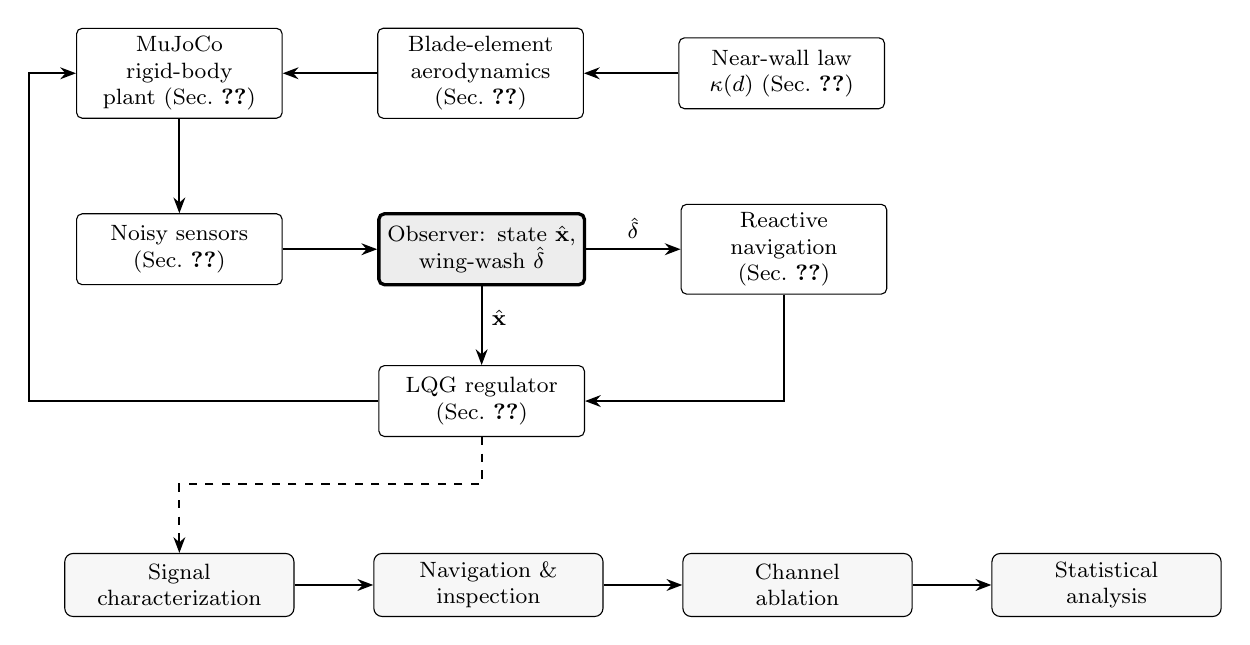
\begin{tikzpicture}[
  font=\footnotesize,
  >={Stealth[length=2mm]},
  blk/.style={draw, rounded corners=2pt, align=center, minimum height=9mm,
              text width=24mm, inner sep=3pt},
  key/.style={draw, rounded corners=2pt, align=center, minimum height=9mm,
              text width=24mm, inner sep=3pt, fill=black!7, very thick},
  grp/.style={draw, rounded corners=3pt, align=center, minimum height=8mm,
              text width=27mm, inner sep=3pt, fill=black!3},
  arr/.style={->, thick},
  darr/.style={->, thick, dashed}
]
% row 1: platform
\node[blk] (plant) {MuJoCo rigid-body\\plant (Sec.~\ref{sec:method_vehicle})};
\node[blk, right=12mm of plant] (aero) {Blade-element\\aerodynamics (Sec.~\ref{sec:method_aero})};
\node[blk, right=12mm of aero] (kappa) {Near-wall law\\$\kappa(d)$ (Sec.~\ref{sec:method_wingwash})};
\draw[arr] (aero) -- (plant);
\draw[arr] (kappa) -- (aero);
% row 2: control and sensing
\node[blk, below=12mm of plant] (sensors) {Noisy sensors\\(Sec.~\ref{sec:method_noise})};
\node[key, right=12mm of sensors] (kf) {Observer: state $\hat{\mathbf{x}}$,\\wing-wash $\hat{\delta}$};
\node[blk, right=12mm of kf] (nav) {Reactive navigation\\(Sec.~\ref{sec:method_nav})};
\draw[arr] (plant) -- (sensors);
\draw[arr] (sensors) -- (kf);
\node[blk, below=10mm of kf] (lqg) {LQG regulator\\(Sec.~\ref{sec:method_control})};
\draw[arr] (kf) -- node[right, pos=0.4] {$\hat{\mathbf{x}}$} (lqg);
\draw[arr] (kf) -- node[above] {$\hat{\delta}$} (nav);
\draw[arr] (nav) |- (lqg.east);
\draw[arr] (lqg.west) -| ($(sensors.west)+(-6mm,0)$) |- (plant.west);
% row 3: evaluation
\node[grp, below=34mm of sensors] (e1) {Signal\\characterization};
\node[grp, right=10mm of e1] (e2) {Navigation \&\\inspection};
\node[grp, right=10mm of e2] (e3) {Channel\\ablation};
\node[grp, right=10mm of e3] (e4) {Statistical\\analysis};
\draw[arr] (e1) -- (e2);
\draw[arr] (e2) -- (e3);
\draw[arr] (e3) -- (e4);
\draw[darr] (lqg.south) -- ++(0,-6mm) -| (e1.north);
\end{tikzpicture}
\caption{Methodology workflow of the flapping-wing sensing and navigation study.}
\label{fig:workflow}
\end{figure*}

\subsection{Simulation Framework and Vehicle Model}
\label{sec:method_vehicle}

The vehicle is modelled in the MuJoCo rigid-body physics engine, which supplies the mass properties, the wing kinematics, and the ray casting used for sensing. The six-degree-of-freedom body dynamics are advanced by a semi-implicit Euler step at the physics timestep, with all aerodynamic forces supplied by the blade-element model of Section~\ref{sec:method_aero}, since the engine does not itself resolve the unsteady low-Reynolds-number flow at this scale. The wings are represented as prescribed-motion, massless aerodynamic surfaces whose kinematics are imposed at each timestep; this choice follows established practice for quasi-steady flapping simulation and avoids a spurious inertial-reaction artefact that arises when finite-mass wings are driven on a free body, while preserving the forces and moments that the wings transmit to the body. Each wing follows a sinusoidal stroke angle $\phi_s(t) = \Phi\cos(2\pi f t)$, with the feathering angle switching smoothly between $\pm45^\circ$ at each stroke reversal; the hover stroke amplitude, $\Phi = 72.6^\circ$, is the value at which the cycle-averaged lift equals the weight. The thrust, roll, and pitch commands act as common-mode amplitude, differential amplitude, and stroke-offset changes respectively, and yaw is commanded through a split-cycle asymmetry. The body frame is defined with its $x$ axis forward, $y$ axis to the left, and $z$ axis upward, with origin at the centre of mass. 

Figure~\ref{fig:model} shows the modelled vehicle and the discretization of its wings. Panel (a) gives the body, the two wings, and the body coordinate frame, with the principal dimensions marked, and panel (b) shows one wing divided into the $N_s = 20$ spanwise blade-element strips used for the aerodynamic computation of Section~\ref{sec:method_aero}, together with the stroke kinematics imposed in hover.

\begin{figure*}[t]
\centering
\begin{subfigure}[b]{0.62\linewidth}
\centering
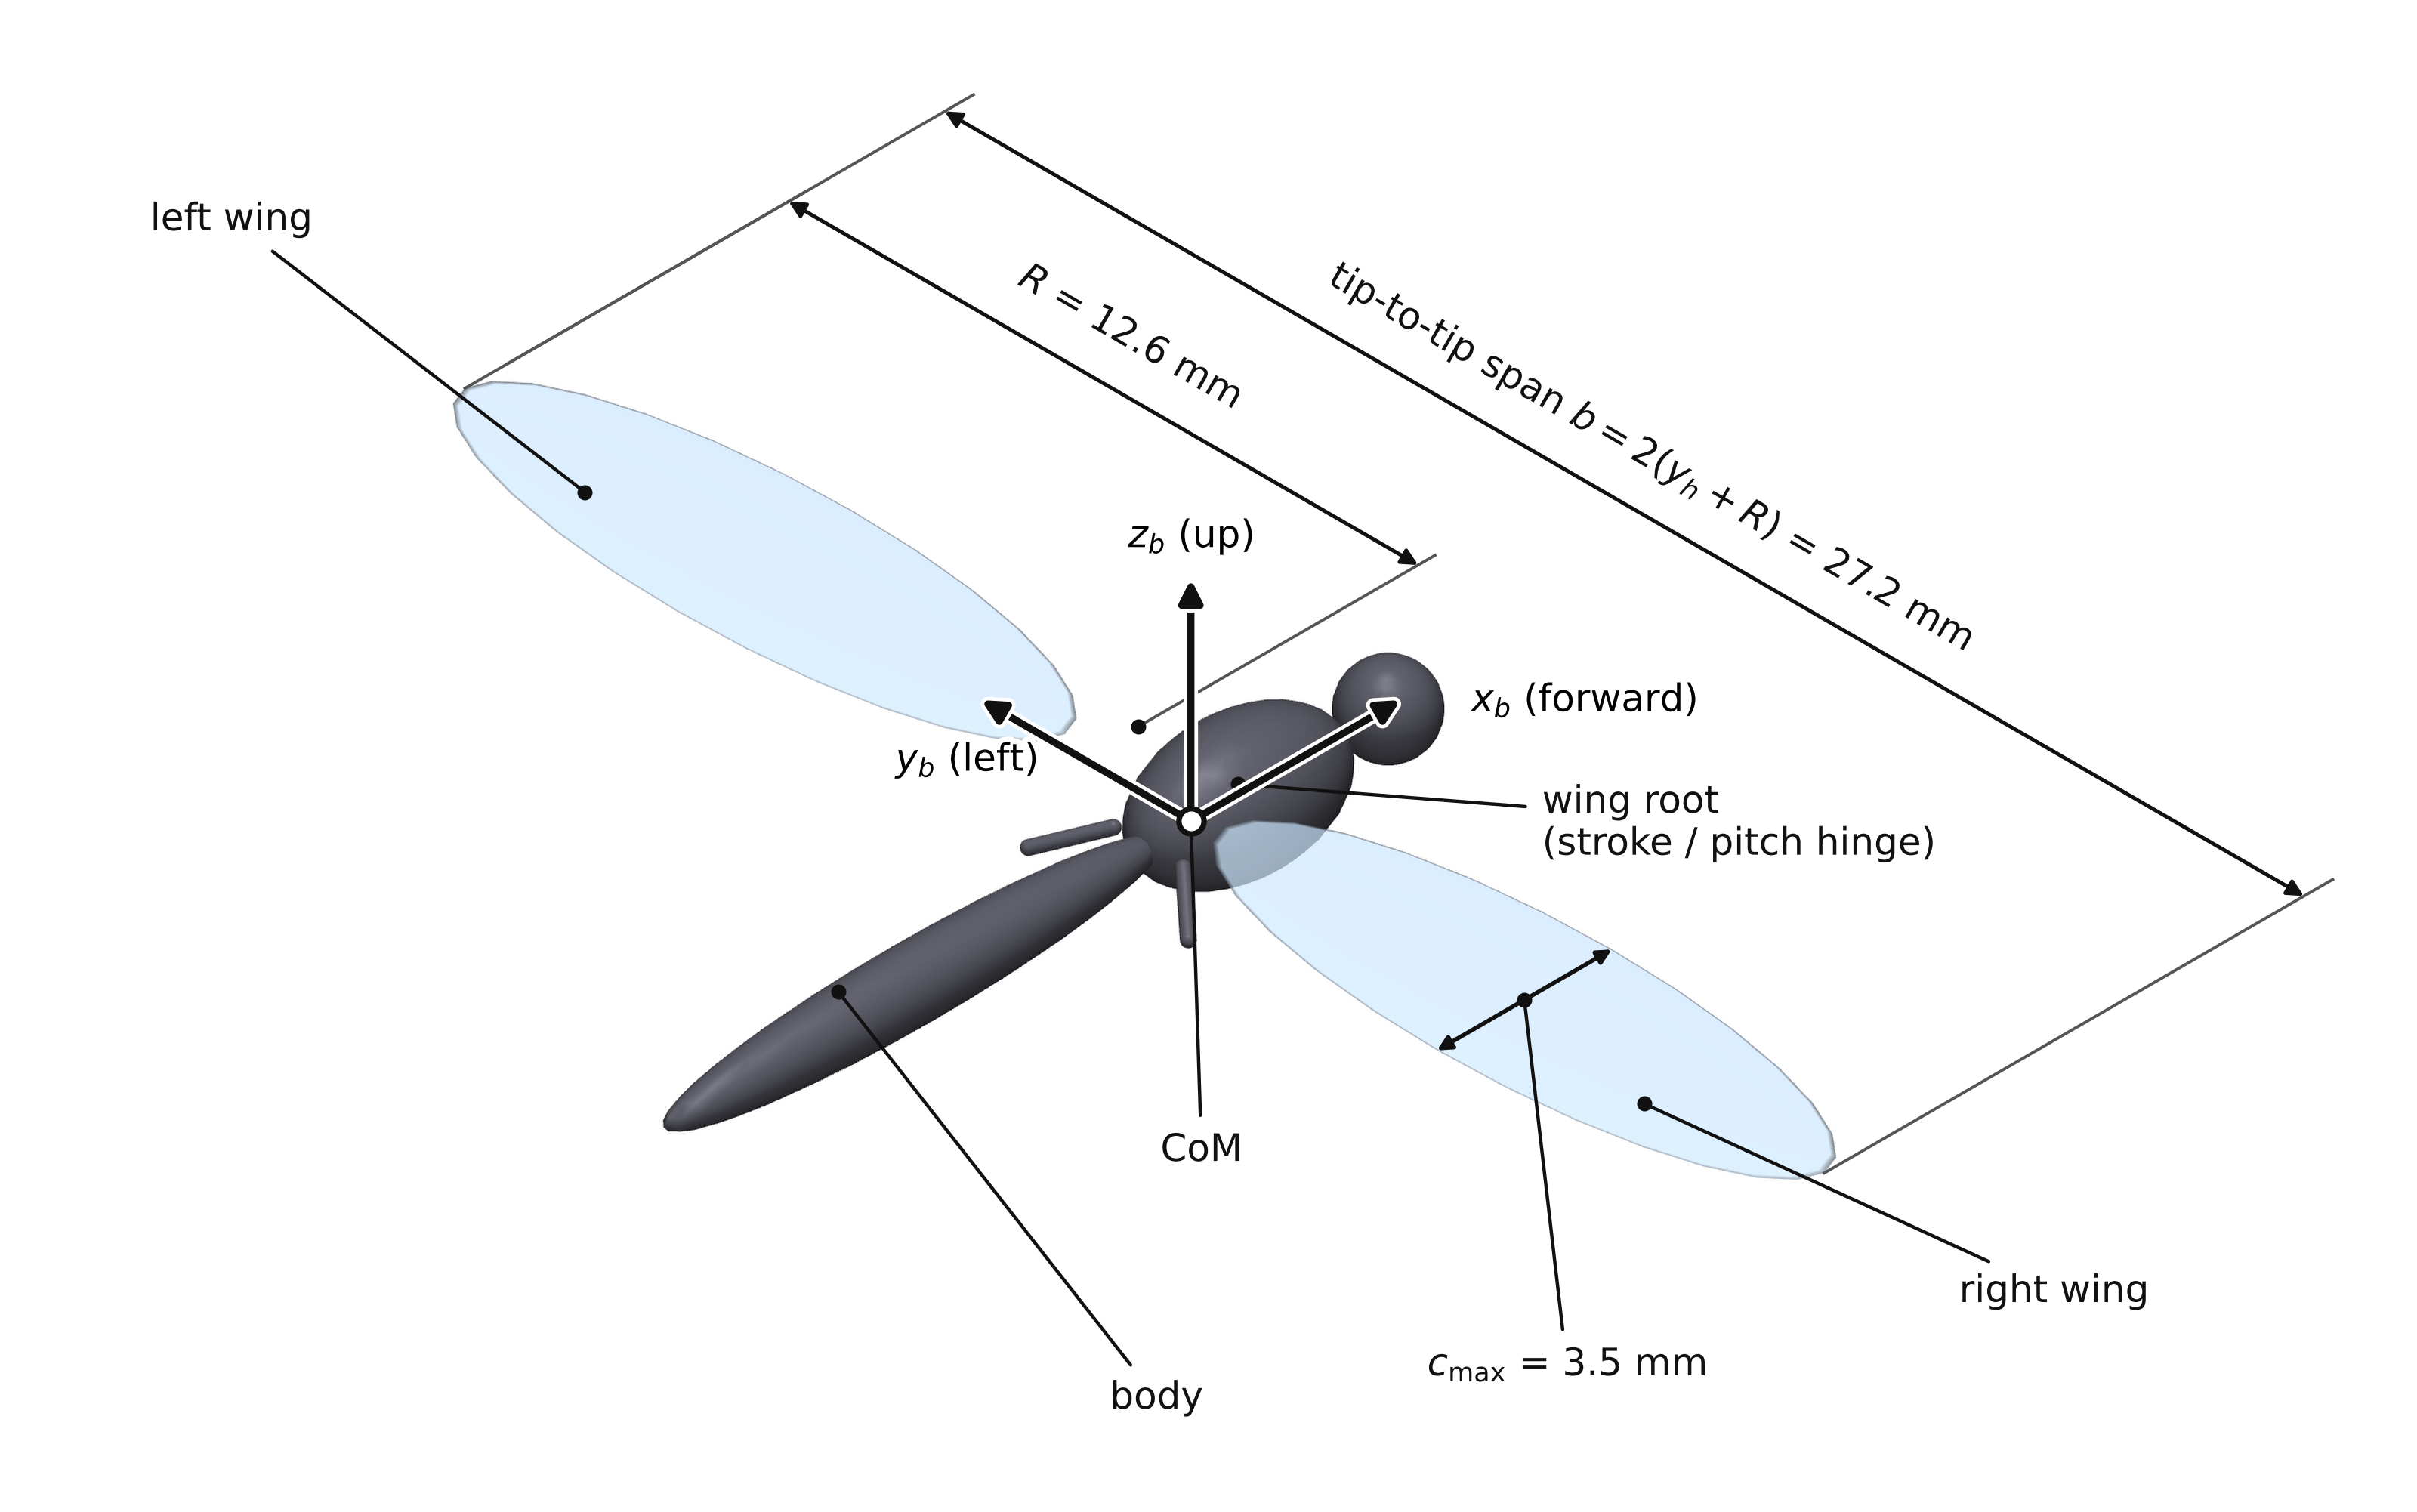
\includegraphics[width=\linewidth]{figures/model_iso.png}
\caption{}
\end{subfigure}\hfill
\begin{subfigure}[b]{0.36\linewidth}
\centering
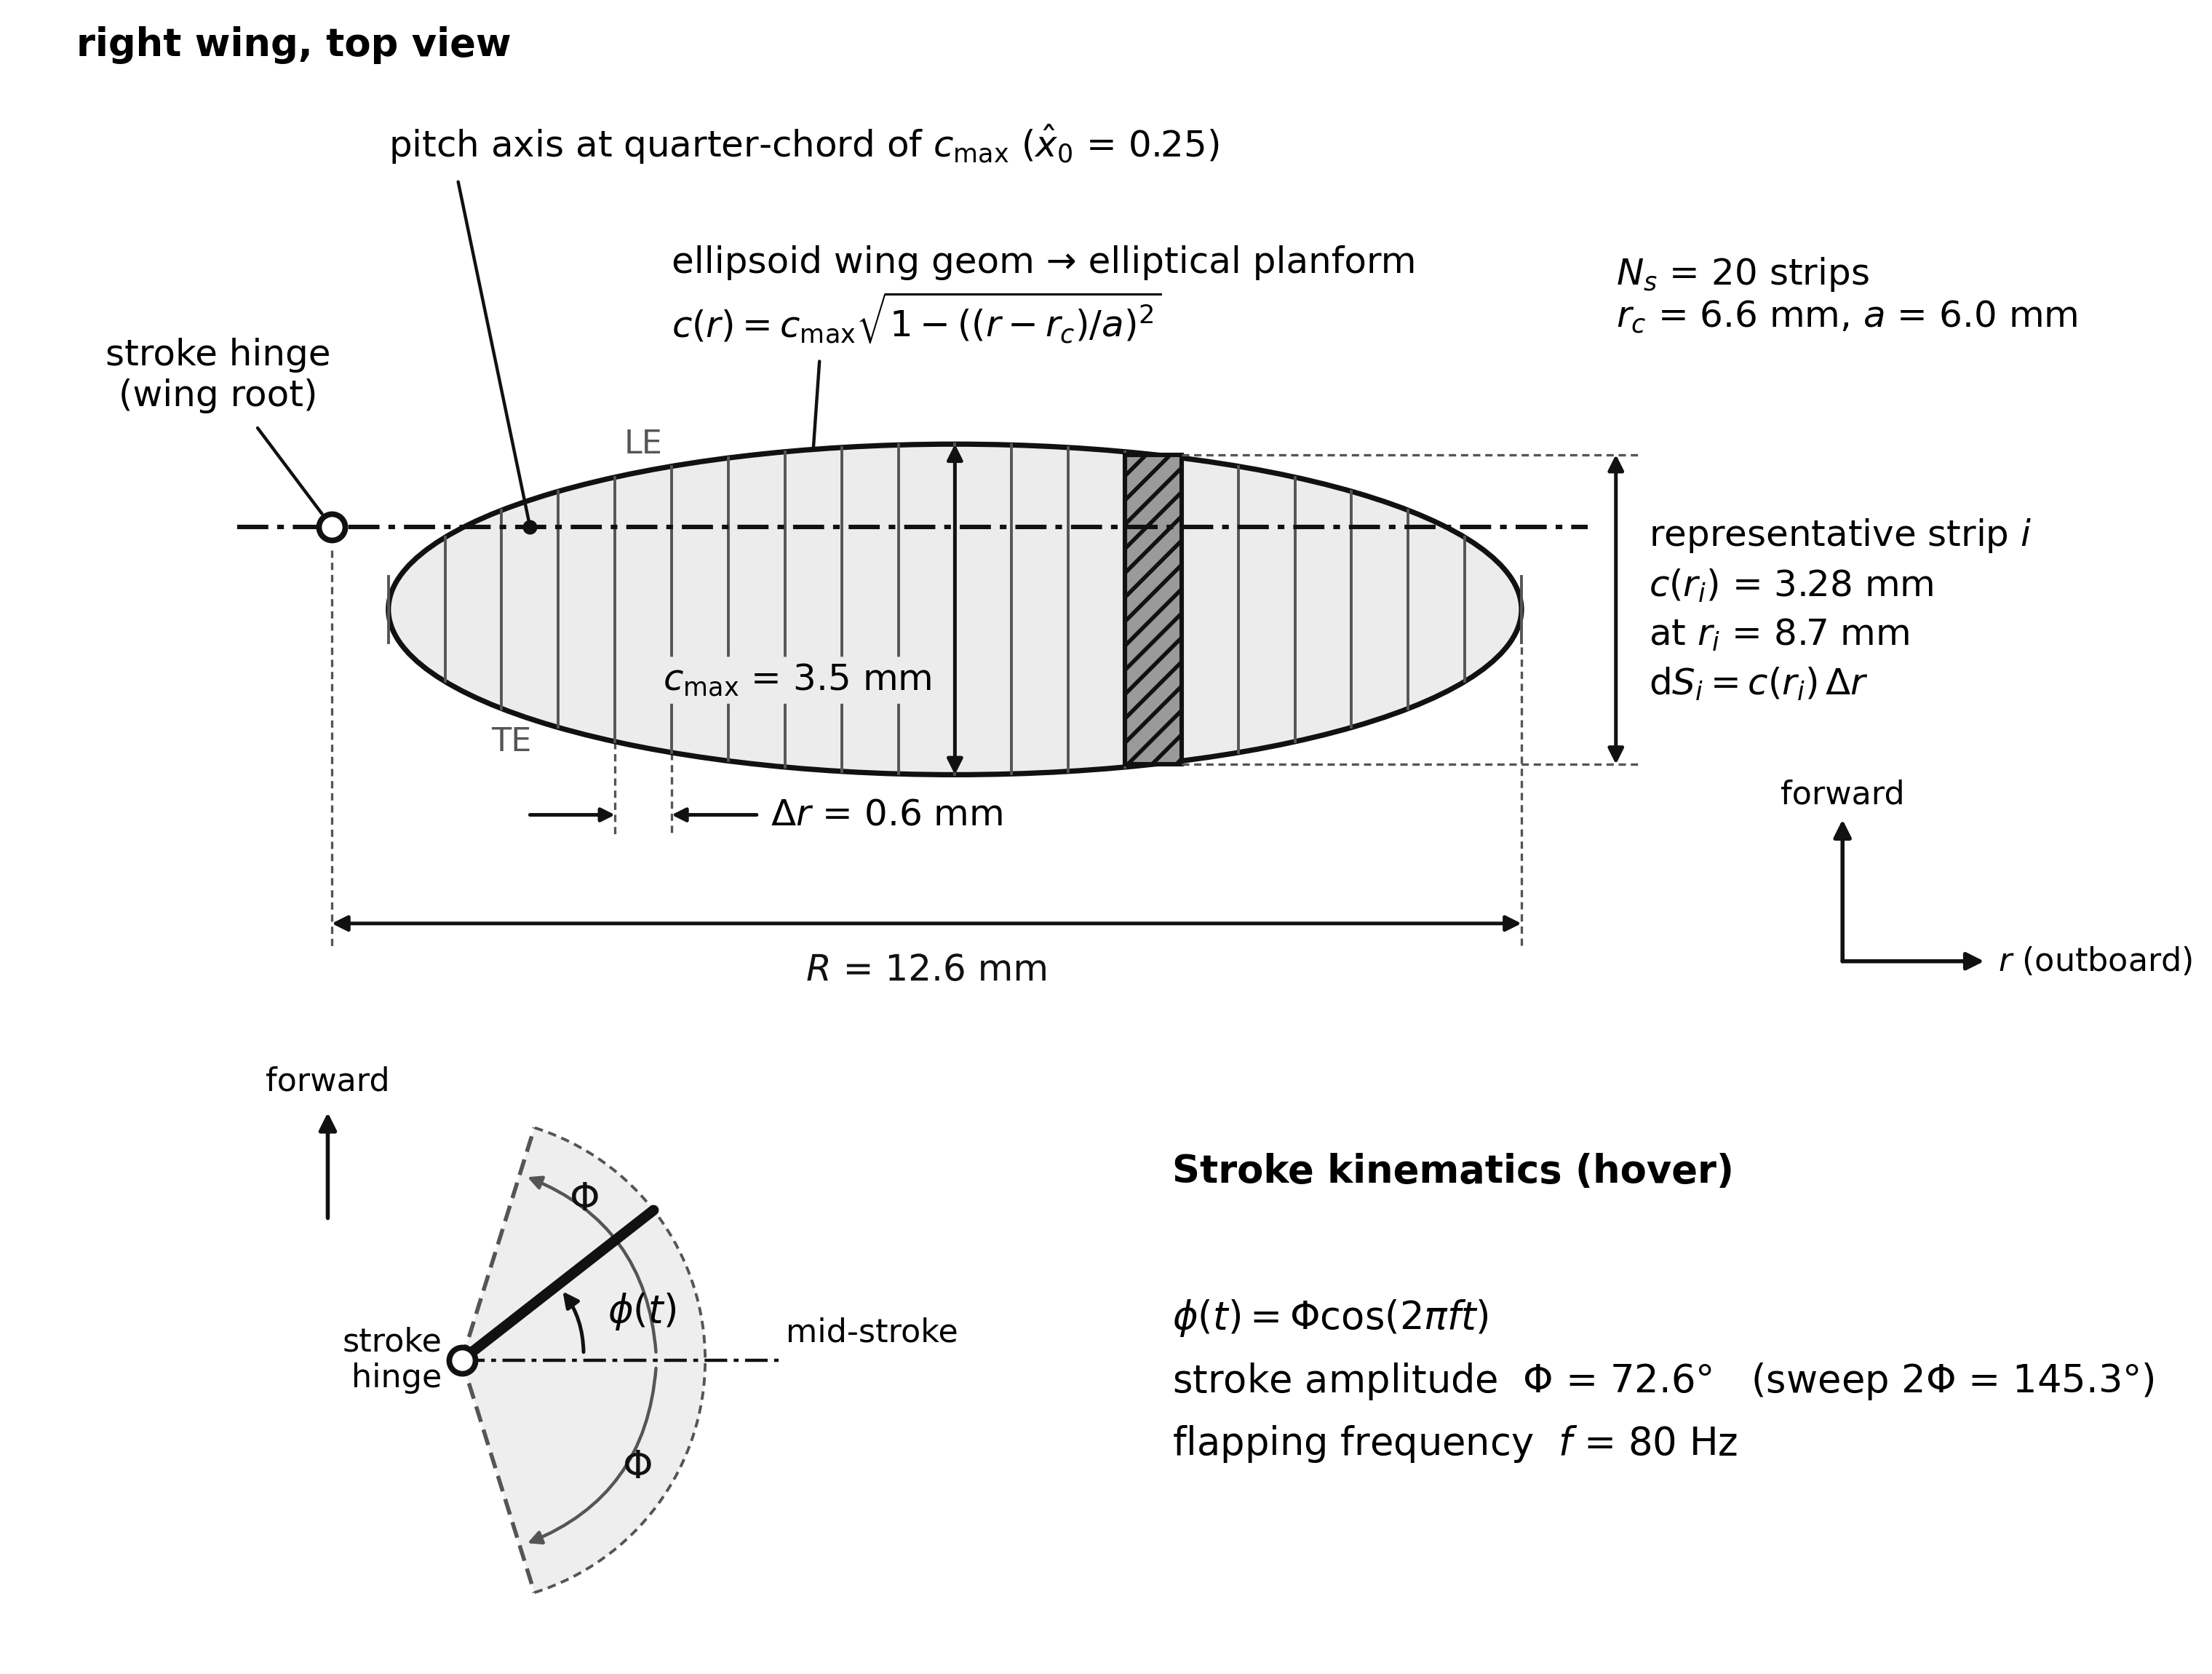
\includegraphics[width=\linewidth]{figures/model_wing_detail.png}
\caption{}
\end{subfigure}
\caption{Simulated vehicle geometry and blade-element wing discretization: (a) body, wings, and body coordinate frame with the principal dimensions and (b) one wing divided into spanwise blade-element strips, with the hover stroke kinematics.}
\label{fig:model}
\end{figure*}

The principal physical parameters of the modelled vehicle are collected in Table~\ref{tab:vehicle}, and are used consistently throughout the aerodynamic and control models that follow.

\begin{table}[t]
\centering
\caption{Physical and operating parameters of the modelled vehicle.}
\label{tab:vehicle}
\footnotesize\setlength{\tabcolsep}{3pt}
\begin{tabular*}{\columnwidth}{@{\extracolsep{\fill}}lll@{}}
\toprule
Parameter & Symbol & Value \\
\midrule
Total mass & $m$ & $77.4$~mg \\
Weight & $mg$ & $759.3~\mu$N \\
Wing length (hinge to tip) & $R$ & $12.6$~mm \\
Hinge offset from centreline & $y_h$ & $1.0$~mm \\
Tip-to-tip span & $2(y_h + R)$ & $27.2$~mm \\
Maximum chord & $c_{\max}$ & $3.5$~mm \\
Strips per wing & $N_s$ & $20$ \\
Roll inertia & $I_{xx}$ & $1.71\times10^{-10}$~kg\,m$^2$ \\
Pitch inertia & $I_{yy}$ & $6.04\times10^{-10}$~kg\,m$^2$ \\
Yaw inertia & $I_{zz}$ & $7.31\times10^{-10}$~kg\,m$^2$ \\
Hover flapping frequency & $f$ & $80$~Hz \\
Cruise speed & $V_c$ & $0.05$~m\,s$^{-1}$ \\
Physics timestep & & $1\times10^{-4}$~s \\
Nominal control rate & & $1$~kHz \\
Wingtip-strike radius & & $13.3$~mm \\
\bottomrule
\end{tabular*}
\end{table}

\subsection{Rigid-Body Dynamics and Linearized Model}
\label{sec:method_dynamics}

The vehicle is treated as a rigid body of mass $m$ with inertia tensor $\mathbf{I}$, whose diagonal is $(I_{xx}, I_{yy}, I_{zz})$; its one non-zero product of inertia, $I_{xz}$, is about one percent of $I_{xx}$ and is retained in the simulation. Writing $\mathbf{p}$ for world-frame position, $\mathbf{v}$ for world-frame velocity, $\boldsymbol{\eta} = [\phi, \theta, \psi]^\top$ for the Euler angles, and $\boldsymbol{\omega}$ for the body angular velocity, the equations of motion are
\begin{equation}
    \dot{\mathbf{p}} = \mathbf{v}, \qquad m\,\dot{\mathbf{v}} = \mathbf{R}(\boldsymbol{\eta})\,\mathbf{F}_b - m g\,\mathbf{e}_3,
    \label{eq:trans}
\end{equation}
\begin{equation}
    \dot{\boldsymbol{\eta}} = \mathbf{W}(\boldsymbol{\eta})\,\boldsymbol{\omega}, \qquad \mathbf{I}\,\dot{\boldsymbol{\omega}} + \boldsymbol{\omega} \times \mathbf{I}\,\boldsymbol{\omega} = \boldsymbol{\tau}_b,
    \label{eq:rot}
\end{equation}
where $\mathbf{R}$ is the body-to-world rotation, $\mathbf{W}$ maps body rates to Euler-angle rates, $\mathbf{e}_3 = [0,0,1]^\top$, and $\mathbf{F}_b$, $\boldsymbol{\tau}_b$ are the aerodynamic force and torque supplied by the blade-element model. For control design, the dynamics are linearized about the nominal hovering condition, giving
\begin{equation}
    \dot{\mathbf{x}}(t) = \mathbf{A}\,\mathbf{x}(t) + \mathbf{B}\,\mathbf{u}(t) + \mathbf{E}\,w(t),
    \label{eq:cont_ss}
\end{equation}
where $\mathbf{x} = [v_x, v_y, v_z, \omega_x, \omega_y, \phi, \theta, z_I]^\top$ collects the velocity, roll-rate and pitch-rate, and roll and pitch perturbations together with the altitude error $z_I$, which is the integral of $v_z$, $\mathbf{u} = [u_T, u_\phi, u_\theta]^\top$ holds the thrust, roll, and pitch commands, and $w(t)$ is a roll-axis disturbance developed in Section~\ref{sec:method_control}. The matrices $\mathbf{A}$ and $\mathbf{B}$ are obtained numerically, by central finite differences of the cycle-averaged aerodynamic wrench with respect to the body velocities, the body rates, and each command about the hover trim. Yaw and yaw rate are excluded from this model and are regulated by a separate heading loop. Because control is applied at a fixed interval $T_c$, the model is discretized exactly under a zero-order hold through a single matrix exponential of the augmented generator,
\begin{equation}
    \begin{bmatrix} \mathbf{A}_d & \mathbf{B}_d \\ \mathbf{0} & \mathbf{I} \end{bmatrix} = \exp\!\left( \begin{bmatrix} \mathbf{A} & \mathbf{B} \\ \mathbf{0} & \mathbf{0} \end{bmatrix} T_c \right),
    \label{eq:zoh}
\end{equation}
so that $\mathbf{A}_d$ and $\mathbf{B}_d$ are exact for the given $T_c$ rather than first-order approximations, which matters when the control interval is lengthened in the sensitivity analysis of Section~\ref{sec:results_sensitivity}.

\subsection{Blade-Element Aerodynamic Model}
\label{sec:method_aero}

The forces produced by each wing are computed with a quasi-steady blade-element model, in which the wing is divided into $N_s$ spanwise strips and the force on each strip is obtained from its local velocity and orientation. The strip at radial station $r$ has chord $c(r)$ and moves, by virtue of the prescribed flapping, with local speed $U_t(r,t) = r\,\dot{\phi}_s(t)$. Three force contributions are modelled: a translational (circulatory) term, which dominates mid-stroke,
\begin{equation}
    \mathrm{d}\mathbf{F}_{\mathrm{trans}} = \tfrac{1}{2}\,\rho\, c(r)\, U_t^2\, \big[ C_L(\alpha)\,\hat{\mathbf{e}}_L + C_D(\alpha)\,\hat{\mathbf{e}}_D \big]\,\mathrm{d}r,
    \label{eq:Ftrans}
\end{equation}
with $C_L(\alpha) = C_{L,\max}\sin 2\alpha$ and $C_D(\alpha) = C_{D,0} + (C_{D,\max} - C_{D,0})\sin^2\alpha$; a rotational term accounting for force generation at stroke reversal,
\begin{equation}
    \mathrm{d}\mathbf{F}_{\mathrm{rot}} = \rho\, C_{\mathrm{rot}}\, c^2(r)\, U_t\, \dot{\alpha}\, \hat{\mathbf{n}}\,\mathrm{d}r, \quad C_{\mathrm{rot}} = \pi\!\left( \tfrac{3}{4} - \hat{x}_0 \right);
    \label{eq:Frot}
\end{equation}
and an added-mass term reflecting the inertia of the displaced fluid,
\begin{equation}
    \mathrm{d}\mathbf{F}_{\mathrm{am}} = -\rho\,\tfrac{\pi}{4}\, c^2(r)\, a_n\, \hat{\mathbf{n}}\,\mathrm{d}r.
    \label{eq:Fam}
\end{equation}
The net force and torque transmitted by one wing are the strip sums $\mathbf{F}_w = \sum_i \mathrm{d}\mathbf{F}_i$ and $\boldsymbol{\tau}_w = \sum_i (\mathbf{r}_i - \mathbf{r}_{\mathrm{cm}}) \times \mathrm{d}\mathbf{F}_i$, and the total wrench is the sum over both wings. The empirical coefficients follow values reported for revolving insect wings, with $C_{L,\max}=1.8$, $C_{D,0}=0.2$, $C_{D,\max}=1.8$, and $\hat{x}_0=0.25$. In free-air hover the two wings are symmetric and produce no net roll torque; it is the breaking of this symmetry by a nearby wall, described next, that produces the sensing signal.

\subsection{Near-Wall Interaction Law}
\label{sec:method_wingwash}

When a wing operates near a surface, its lift is modified relative to the free-air value, an effect that is distance-dependent and well established for flapping-wing flight \cite{cheeseman1959effect, maeda2013ground, lu2016ground}. Adopting the classical ground-effect relation at the level of the individual strip, the translational lift of a strip at perpendicular distance $d$ from a wall is scaled by
\begin{equation}
    \kappa(d) = \min\!\left( 1 + K_{\mathrm{GE}} \left( \frac{R}{4d} \right)^2,\; \kappa_{\max} \right),
    \label{eq:kappa}
\end{equation}
with $K_{\mathrm{GE}} = 1.0$ and $\kappa_{\max} = 2.0$ throughout, where $\kappa_{\max}$ caps the enhancement at close range to prevent the non-physical divergence of the expression as $d\to 0$. It is stated plainly that Eq.~\eqref{eq:kappa} is imposed rather than derived: the simulation does not compute the near-wall flow but applies this scalar multiplier to the modelled translational lift of each strip, leaving the drag, rotational, and added-mass terms unchanged, so $K_{\mathrm{GE}}$ is the single parameter on which the quantitative characterization depends, and its influence is examined explicitly. When the vehicle sits beside a wall, the strips of the near wing lie at smaller distances than those of the far wing and are enhanced more strongly, and the resulting left-right asymmetry produces a net body-axis roll torque,
\begin{equation}
    \tau_x^{\mathrm{wall}} \approx \sum_{i} \big( \kappa(d_i) - 1 \big)\, \mathrm{d}F_{z,i}\, y_i,
    \label{eq:tauwall}
\end{equation}
written here as the far-field, vertical-lift reduction of the exact moment that the implementation forms as a cross-product sum over strips. The sign of $\tau_x^{\mathrm{wall}}$ indicates which side the wall lies on, and its magnitude varies with distance, so the roll torque is a distance-dependent, side-resolving proximity signal produced by the vehicle's own propulsion. This torque appears to the controller as an external disturbance and is recovered by the observer of Section~\ref{sec:method_control}, which is what makes it available for navigation. This study refers to it as the wing-wash signal. Figure~\ref{fig:sensing} illustrates this geometry. The near wing, lying at smaller strip distances $d_i$, is enhanced more strongly than the far wing, and the resulting left-right lift asymmetry produces the roll torque $\tau_x^{\mathrm{wall}}$ that rolls the vehicle away from the wall; the same panel shows the seven feeler rays that provide the complementary tactile cue.

\begin{figure}[t]
\centering
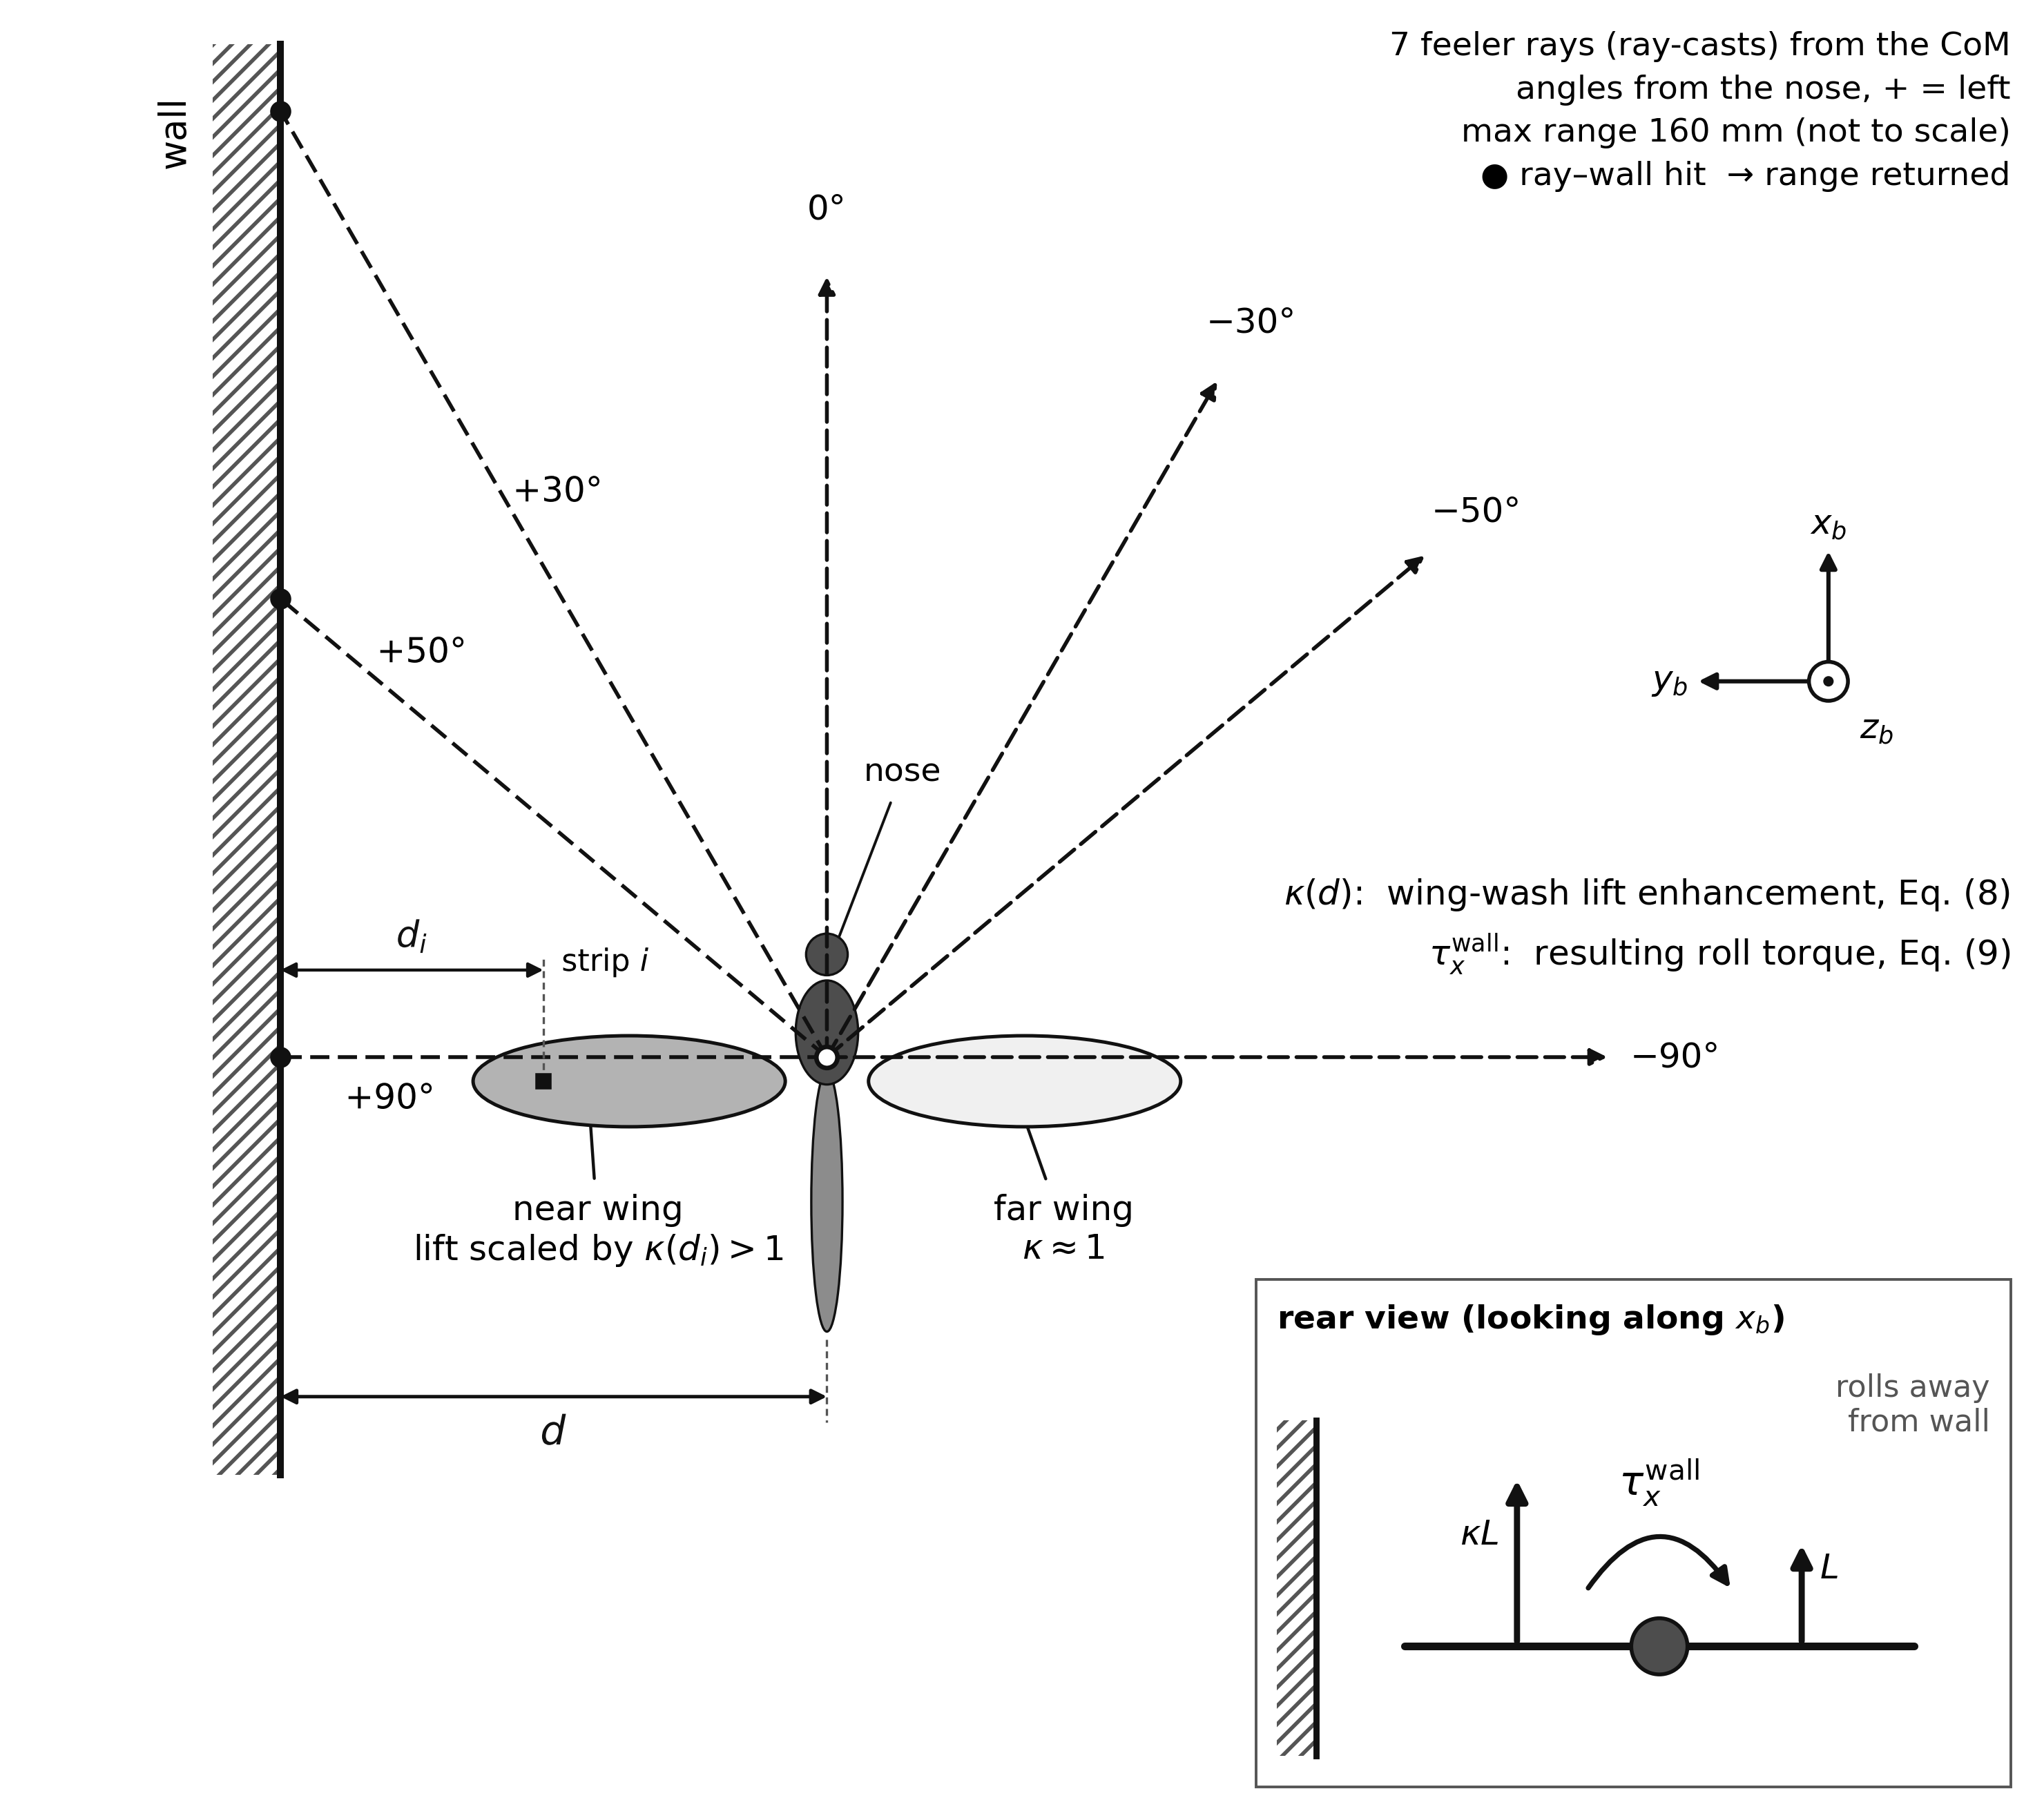
\includegraphics[width=\linewidth]{figures/model_sensing_geometry.png}
\caption{Wing-wash asymmetry and feeler-ray sensing geometry.}
\label{fig:sensing}
\end{figure}

\subsection{Control and Disturbance Estimation}
\label{sec:method_control}

Stabilized flight uses a linear-quadratic-Gaussian (LQG) regulator acting on a Kalman-filter state estimate. The regulator gain $\mathbf{K}$ minimizes the infinite-horizon discrete cost $J = \sum_{k} ( \mathbf{x}_k^\top \mathbf{Q}\,\mathbf{x}_k + \mathbf{u}_k^\top \mathbf{R}_u\,\mathbf{u}_k )$, obtained from the discrete algebraic Riccati equation, with the diagonal weights $\mathbf{Q}$ and $\mathbf{R}_u$ chosen to produce a stable hovering operating point. The element on which the sensing idea depends is the disturbance observer. The estimator state is augmented with a roll-axis disturbance $\delta$, modelled as slowly varying,
\begin{equation}
    \begin{bmatrix} \mathbf{x}_{k+1} \\ \delta_{k+1} \end{bmatrix} = \begin{bmatrix} \mathbf{A}_d & \mathbf{E}_d \\ \mathbf{0} & 1 \end{bmatrix} \begin{bmatrix} \mathbf{x}_k \\ \delta_k \end{bmatrix} + \begin{bmatrix} \mathbf{B}_d \\ \mathbf{0} \end{bmatrix} \mathbf{u}_k + \begin{bmatrix} \mathbf{0} \\ 1 \end{bmatrix} w^{\delta}_k,
    \label{eq:aug}
\end{equation}
and the augmented Kalman filter returns, each step, an estimate $\hat{\delta}_k$ alongside the state estimate $\hat{\mathbf{x}}_k$. The estimator gain is computed from the continuous-time counterpart of Eq.~\eqref{eq:aug} through the algebraic Riccati equation, and the estimator is then propagated over each control interval under an exact zero-order hold. The control law regulates the estimated state while feeding the estimated disturbance forward for rejection, $\mathbf{u}_k = -\mathbf{K}\,\hat{\mathbf{x}}_k - \mathbf{K}_{\delta}\,\hat{\delta}_k + \mathbf{u}_{\mathrm{ref},k}$, where $\mathbf{u}_{\mathrm{ref},k}$ is the reference from the navigation layer. The key point, in the manner of disturbance-observer-based methods \cite{chen2015disturbance}, is that $\hat{\delta}_k$ is not merely a quantity to reject: when a wall is present it estimates the wall-induced torque of Eq.~\eqref{eq:tauwall}, so the same estimator that stabilizes the vehicle also measures its lateral surroundings. No component of this architecture is learned; all gains follow analytically from the linearized model. The deployed weights, which differ from the source-module defaults, are reported in Table~\ref{tab:params} so that the controller is reproducible.

Figure~\ref{fig:hover} illustrates the stabilizing action of a regulator of this architecture in free air; this demonstration uses the source-module default weights and not the deployed weights of Table~\ref{tab:params}. Released with a $10^\circ$ attitude offset in both pitch and roll, the uncontrolled vehicle diverges past $45^\circ$ within about $124$~ms, whereas the regulated vehicle settles to hover and rejects a roll gust and a pitch gust applied at $400$ and $800$~ms while holding its height within about $1$~mm of the $50$~mm reference.

\begin{figure}[t]
\centering
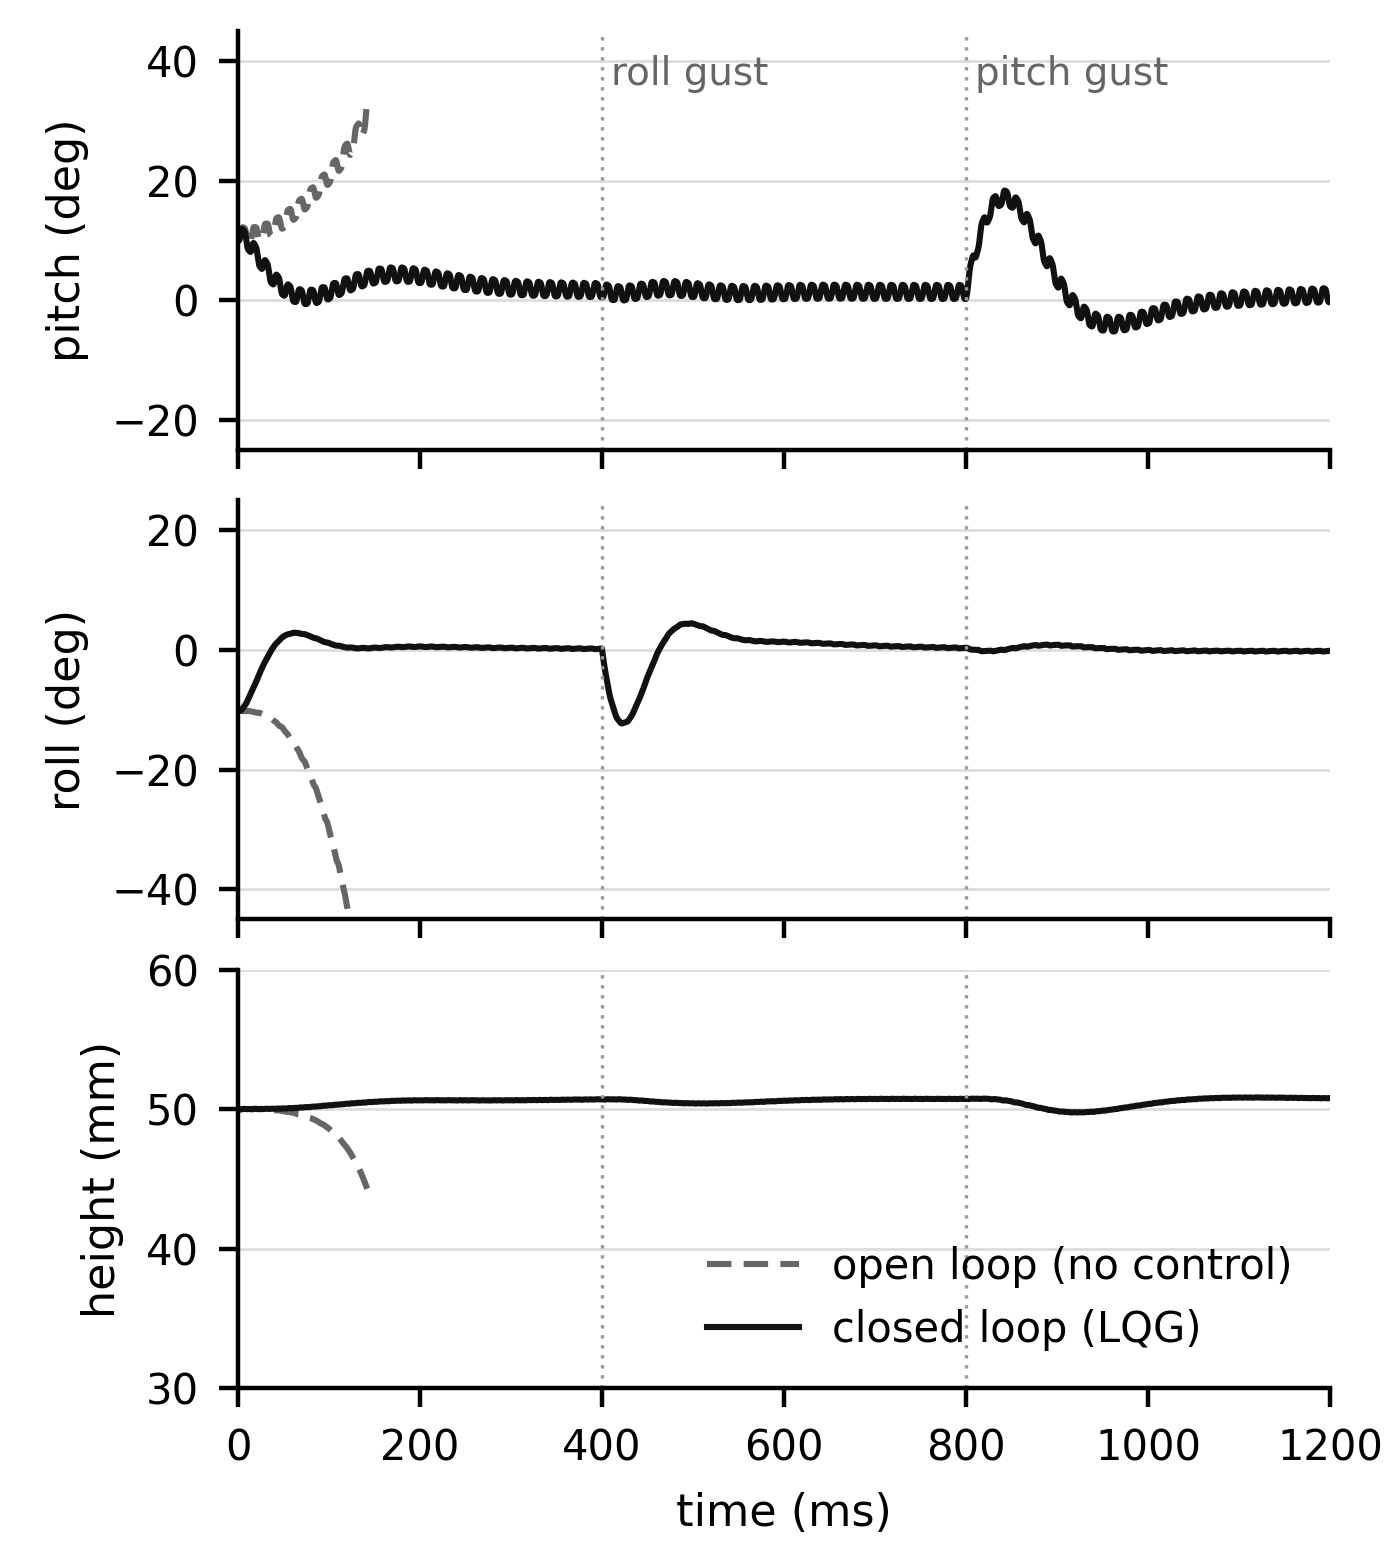
\includegraphics[width=\linewidth]{figures/fig03_hover_control.png}
\caption{Open-loop divergence and closed-loop LQG hover with gust rejection.}
\label{fig:hover}
\end{figure}

\subsection{Sensor Suite and Noise Model}
\label{sec:method_noise}

The vehicle carries two sensory channels. The first is the aerodynamic proximity channel, which is not a physical sensor but the roll-axis disturbance estimate of Section~\ref{sec:method_control}, and therefore adds no mass or power. The second is a set of seven feelers, modelled as rays cast from the centre of mass at $0^\circ$, $\pm30^\circ$, $\pm50^\circ$, and $\pm90^\circ$ to the heading, so that the outermost pair points sideways, each returning the distance to the first wall it meets up to a maximum range of $0.16$~m. It is stated at the outset, and revisited in the ablation, that these feelers are idealized: they return exact geometric range through free space, rather than the contact or bending signals of a physical tactile antenna. With a nominal range of about six times the vehicle's span, the modelled channel behaves more like a short-range rangefinder than a contact sensor, which is why its range is the property degraded in Sections~\ref{sec:results_regimes} and~\ref{sec:results_confirm}. All measurements are corrupted by an additive Gaussian noise model,
\begin{equation}
    \tilde{y}_{j,k} = y_{j,k} + \nu_{j,k}, \qquad \nu_{j,k} \sim \mathcal{N}\!\left(0, (\lambda\,\sigma_j)^2\right),
    \label{eq:noise}
\end{equation}
where $\sigma_j$ is the baseline standard deviation of channel $j$, listed in Table~\ref{tab:noise}, and $\lambda$ is a multiplier, set to unity, the nominal condition, in every closed-loop result reported here. This noise model is an assumption of the study rather than a hardware measurement, and the aerodynamic estimate is never noised directly; noise reaches it only through the inertial measurements and the estimator, which is the physically faithful path.

\begin{table}[t]
\centering
\caption{Baseline standard deviations of the sensor-noise model at $\lambda = 1$.}
\label{tab:noise}
\footnotesize\setlength{\tabcolsep}{3pt}
\begin{tabular*}{\columnwidth}{@{\extracolsep{\fill}}lll@{}}
\toprule
Measurement channel & $\sigma_j$ & Unit \\
\midrule
Feeler range & $0.002$ & m \\
Attitude (pitch, roll) & $0.005$ & rad \\
Angular rate & $0.020$ & rad\,s$^{-1}$ \\
Translational velocity & $0.005$ & m\,s$^{-1}$ \\
Heading & $0.005$ & rad \\
Height & $0.001$ & m \\
\bottomrule
\end{tabular*}
\end{table}

\subsection{Reactive Navigation Layer}
\label{sec:method_nav}

The navigation layer maps instantaneous sensory inputs to attitude and velocity references through fixed reactive laws, with no map, planner, or learned policy, and is built so that either channel may be disabled independently for the ablation. Lateral centring drives the low-pass-filtered wing-wash estimate toward zero while damping lateral velocity, subject to a small roll saturation. Forward speed is reduced as the forward feeler approaches an obstacle, and heading is steered toward the more open of the two forward diagonals, so corridors are followed and corners are turned. When the forward path is blocked and a side is open, the geometry is a junction and the vehicle turns into it; when the forward path is clear and exactly one side reads open, it is an opening in an intact wall, and the vehicle holds its line under a feeler-vetoed law that follows the remaining wall while logging the opening. This arbitration between an opening to inspect and a passage to follow is the mechanism on which the inspection task rests.

The fixed values of these reactive laws, together with the regulator and estimator weights of Section~\ref{sec:method_control}, are collected in Table~\ref{tab:params}. They are the values used in every closed-loop flight reported here, and none is changed between sensing configurations.

\begin{table*}[t]
\centering
\begin{threeparttable}
\caption{Regulator, estimator, and navigation parameters as deployed in all closed-loop flights.}
\label{tab:params}
\footnotesize\setlength{\tabcolsep}{3.5pt}
\begin{tabular*}{\textwidth}{@{\extracolsep{\fill}}lll@{}}
\toprule
Parameter & Value & Applies to \\
\midrule
\multicolumn{3}{@{}l}{\emph{LQG regulator}} \\
State weights $\mathbf{Q}$ (diagonal)\tnote{a} & $150,\ 150,\ 20,\ 2,\ 2,\ 250,\ 250,\ 6\times10^{4}$ & $v_x, v_y, v_z, \omega_x, \omega_y, \phi, \theta$, $z_I$ \\
Input weights $\mathbf{R}_u$ (diagonal) & $50,\ 50,\ 50$ & thrust, roll, pitch commands \\
\midrule
\multicolumn{3}{@{}l}{\emph{Kalman filter and disturbance observer}} \\
Process-noise weights (diagonal) & $1,\ 1,\ 0.05,\ 30,\ 30,\ 0.02,\ 0.02,\ 10^{-6}$ & same state ordering as $\mathbf{Q}$ \\
Disturbance process-noise weight & $2\times10^{8}$ & roll-axis disturbance $\delta$ \\
Measurement-noise weights (diagonal) & $10^{-3},\ 100,\ 100,\ 10^{-4},\ 10^{-4},\ 10^{-7}$ & $v_z, \omega_x, \omega_y, \phi, \theta$, altitude \\
Wing-wash low-pass time constant & $0.10$~s & $\hat{\delta}$ before the centring law \\
\midrule
\multicolumn{3}{@{}l}{\emph{Reactive navigation}} \\
Centring gain & $1.5\times10^{-5}$~s$^{2}$ & roll reference per unit filtered $\hat{\delta}$ \\
Lateral-velocity damping & $3.0$~rad\,s\,m$^{-1}$ & roll reference \\
Roll-reference saturation & $\pm 2.5^\circ$ & cruise ($\pm 2^\circ$ while turning) \\
Steering gain & $5.0$~rad\,s$^{-1}$\,m$^{-1}$ & difference of the $\pm30^\circ$ feelers, each clipped at $0.11$~m \\
Stop and clear distances & $0.042$~m, $0.090$~m & forward feeler: slow to a stop, resume cruise \\
Safety buffer and veer rate & $0.020$~m, $0.9$~rad\,s$^{-1}$ & side and $\pm50^\circ$ feelers \\
Turn yaw rate & $0.5$~rad\,s$^{-1}$ & pivot at a blocked corner \\
Opening threshold & $0.10$~m & side-feeler range above which a wall reads open \\
Wall-follow gain and standoff & $2.0$~rad\,m$^{-1}$, $0.030$~m & feeler-vetoed law beside an opening \\
Cruise height & $0.05$~m & altitude reference \\
Detection match tolerance & $60$~mm & logged to true opening midpoint \\
\bottomrule
\end{tabular*}
\begin{tablenotes}\footnotesize
\item[a] In navigation flights the regulator's feedback on the horizontal velocities $v_x$ and $v_y$ is set to zero, and those velocities are commanded by the navigation layer instead.
\end{tablenotes}
\end{threeparttable}
\end{table*}

\subsection{Experimental Design}
\label{sec:method_experiments}

The evaluation is organized as the sequence of experiment groups shown in Figure~\ref{fig:workflow} and summarized in Table~\ref{tab:experiments}. The first group characterizes the wing-wash signal as an instrument. Its static and two-wall responses are computed with the vehicle held at prescribed poses, in isolation from closed-loop dynamics, while its noise floor and the fidelity of the observer are measured in regulated hover, since they depend on the estimator. The second evaluates reactive navigation and opening inspection, first on crafted courses and then across a randomized ensemble of passages. Each randomized course is generated by independently sampling the number of legs, the turn directions, the corridor widths, and the number, side, position, and length of the wall openings, subject to constraints that keep the geometry realizable, and each course is flown once, so the ensemble measures performance across geometries rather than repeatability on one. The third group ablates each sensing channel in turn on geometrically identical courses, using the same generator and flight seeds across configurations, so the comparison isolates the contribution of a channel rather than the effect of a re-tuned controller; no gain is retuned for any configuration. The fourth group applies the statistical analysis described below, including a confirmatory test, an exploratory gain sweep, and a corridor-width sweep that followed from the ablation.

\begin{table}[t]
\centering
\caption{Numerical experiment groups and the quantities each measures.}
\label{tab:experiments}
\footnotesize\setlength{\tabcolsep}{3pt}
\begin{tabularx}{\columnwidth}{@{}L{2.4cm}Y@{}}
\toprule
Group & Principal quantities \\
\midrule
Signal characterization & Range, resolution, observer gain, two-wall superposition \\
Navigation \& inspection & Completion, strike-free completion, detection, localization \\
Channel ablation & Attribution across full, no-wing-wash, no-feelers, open-loop \\
Statistical analysis & Paired differences, confidence intervals, equivalence, confirmatory test \\
\bottomrule
\end{tabularx}
\end{table}

The sampling distributions of the course generator are listed in Table~\ref{tab:generator}, for the primary ensemble and for the leg-sweep ensemble used in Section~\ref{sec:results_regimes}; the two differ only in leg count and corridor width.

\begin{table}[t]
\centering
\caption{Sampling distributions of the randomized-course generator.}
\label{tab:generator}
\footnotesize\setlength{\tabcolsep}{3pt}
\begin{tabularx}{\columnwidth}{@{}lYY@{}}
\toprule
Quantity & Primary ensemble & Leg sweep \\
\midrule
Courses & $40$ & $100$ ($20$ per leg count) \\
Number of legs & $2$ or $3$, equal probability & $2, 3, 4, 5, 6$ (fixed per cell) \\
Corridor width, per leg & uniform, $64$ to $76$~mm & uniform, $58$ to $64$~mm \\
Leg length & \multicolumn{2}{l}{uniform, $160$ to $260$~mm} \\
Turn direction & \multicolumn{2}{l}{left or right, equal probability} \\
Openings per leg & \multicolumn{2}{l}{$0$ (probability $0.4$) or $1$ ($0.6$)} \\
Opening side & \multicolumn{2}{l}{left or right, equal probability} \\
Opening length & \multicolumn{2}{l}{uniform, $15$ to $90$~mm} \\
Opening centre & \multicolumn{2}{l}{uniform, $0.40$ to $0.62$ of leg length} \\
Opening retained if & \multicolumn{2}{l}{span within $0.25$ to $0.82$ of leg length} \\
Course accepted if & \multicolumn{2}{l}{non-adjacent legs apart; $\geq 1$ opening} \\
\bottomrule
\end{tabularx}
\end{table}

Figure~\ref{fig:courses} shows a sample of the generated primary-ensemble courses, illustrating the range of leg counts, turn directions, and wall-opening placements evaluated.

\begin{figure}[t]
\centering
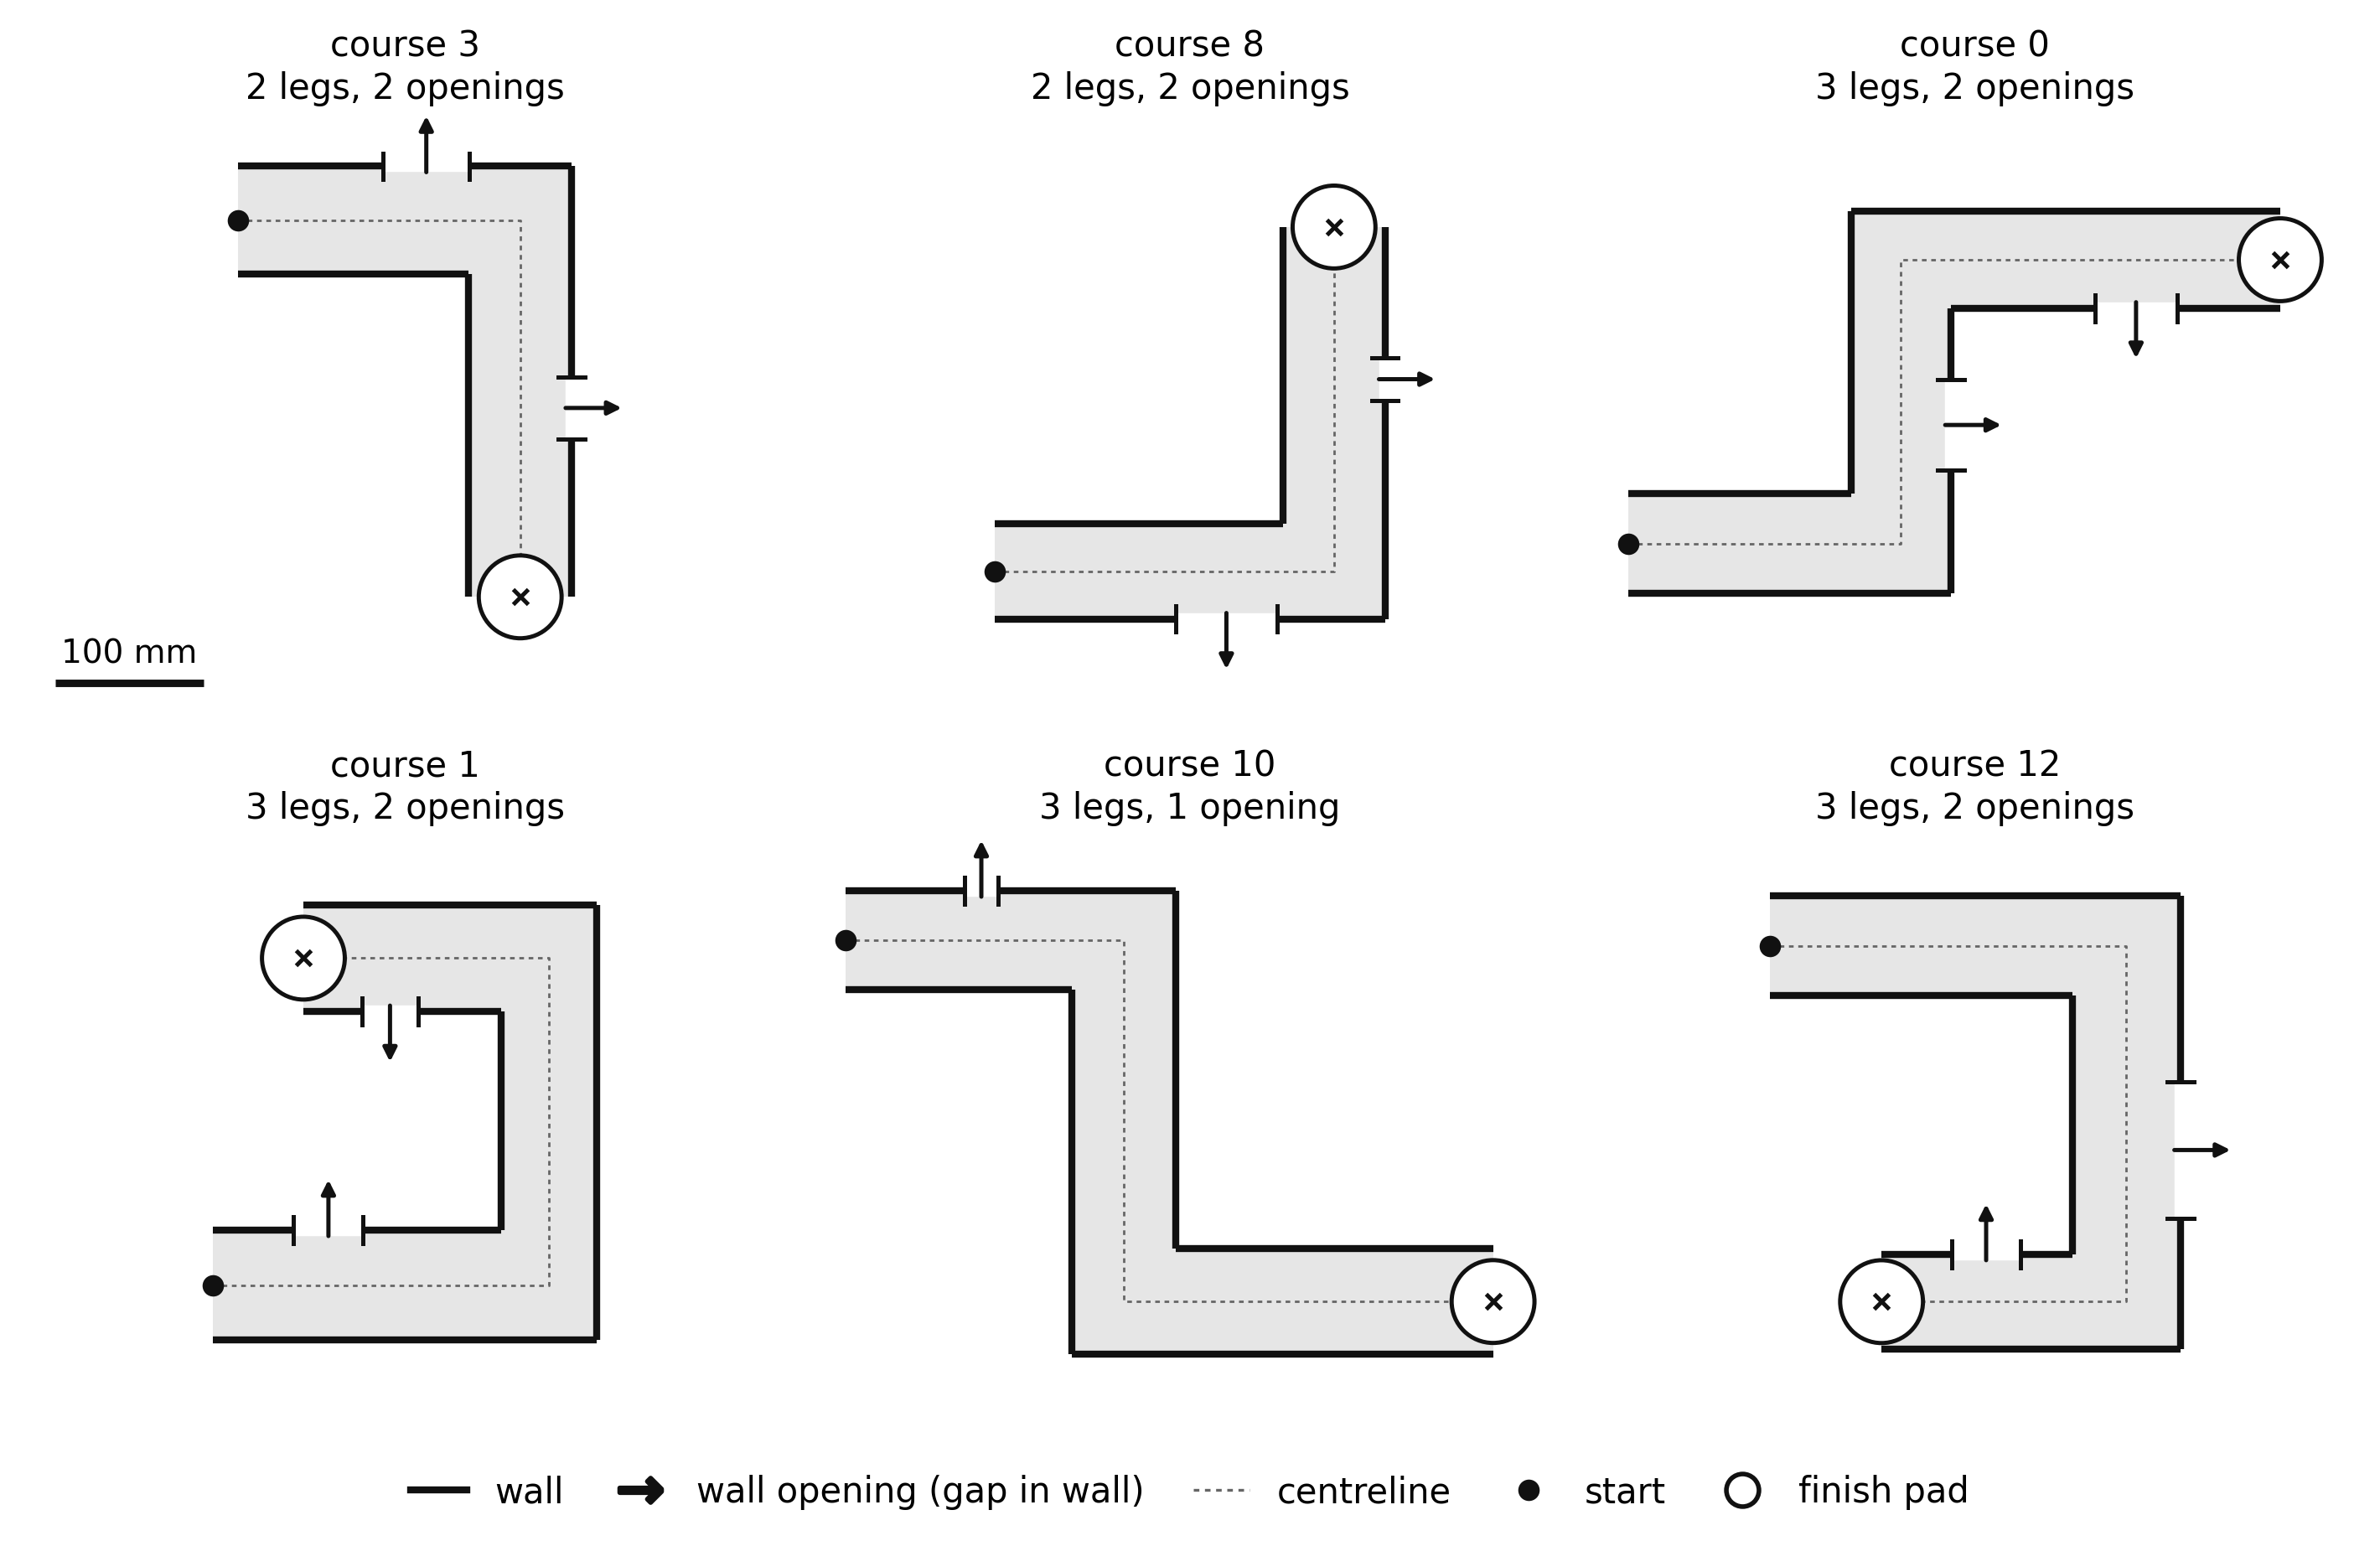
\includegraphics[width=\linewidth]{figures/design_a_courses.png}
\caption{Representative randomized courses from the primary ensemble.}
\label{fig:courses}
\end{figure}

\subsection{Metrics and Statistical Analysis}
\label{sec:method_stats}

Two outcome quantities are kept distinct throughout. A run is a \emph{completion} if the vehicle reaches the goal; a \emph{wingtip strike} is registered when the centre-of-mass-to-wall distance falls below the wingtip-strike radius, under the sampling and the exception stated below; and a run is \emph{strike-free} only if it completes with no strike. For inspection, a logged detection is matched to a ground-truth opening when it lies on the same wall and within a fixed tolerance of the true midpoint, and the per-passage and per-opening detection rates are reported in both their conditional form, over completed courses, and their end-to-end form, over all generated courses.

The scoring rules behind these quantities are stated in full, since several of them affect the reported rates. A flight is a completion when the centre of mass comes within $34$~mm of the goal point inside a time budget of three times the path length divided by the cruise speed, plus $16$~s; a flight that exhausts the budget, or leaves the altitude range of $0$ to $0.2$~m, is not a completion. Clearance is the horizontal distance from the centre of mass to the nearest wall, taken over $24$ rays at $15^\circ$ spacing and sampled every $40$~ms, so a contact that falls between samples or between rays can be missed. A wingtip strike is registered when a sampled clearance falls below the $13.3$~mm strike radius, with one exception: samples taken within $50$~mm of the goal point are not counted as strikes, although they do enter the reported minimum clearance. The strike radius is also slightly smaller than the $13.6$~mm that the wingtip reaches from the centreline at mid-stroke, so the scoring is lenient by about $0.3$~mm. The effect of both choices on the central comparison and on the confirmatory test is reported in Sections~\ref{sec:results_stats} and~\ref{sec:results_confirm}. For inspection, an opening is logged only if the open reading persists over more than $3$~mm of travel, and a logged detection is matched to a true opening when it lies on the same wall and its midpoint is within $60$~mm of the true midpoint. Each logged detection is matched to at most one opening, the nearest, and unmatched detections count as false positives. Detections are scored only on completed flights, and missed openings contribute no localization error. The $60$~mm tolerance is wide against openings of $15$ to $90$~mm, so the detection rate should be read together with the localization error, and the distribution of that error is reported in Section~\ref{sec:results_batch}.

The central comparison, between the full configuration and the configuration with the aerodynamic channel removed, is analysed under a pre-specified paired design: for each course the two configurations are flown under matched noise seeds, and the paired difference in strike-free completion is reported with a 95\% confidence interval obtained by cluster bootstrap over courses ($10{,}000$ resamples, percentile method), together with an exact McNemar test and an equivalence margin of $\pm 5$ percentage points. The analysis and its decision rule were written down before the corresponding flights were launched; the plan was kept with the project and was not lodged with an external registry, so it is described here as pre-specified and not as pre-registered.

The comparison is made on a corrected simulation harness. In the original harness, the wall planes supplied to the near-wall aerodynamic model were reconstructed from the noised lateral feeler readings, so feeler noise perturbed the aerodynamic force itself and the two channels were coupled in the plant and not only in the controller. In the corrected harness the aerodynamic model takes the wall planes from the true ray-cast geometry, and feeler noise or degradation affects only the readings supplied to navigation. All closed-loop results reported here are from the corrected harness; one earlier result that did not survive the correction is identified where it arises.

Three follow-up experiments were specified in the same way after the main comparison. The first is a confirmatory test of a single hypothesis raised by the exploratory feeler-degradation sweep of Section~\ref{sec:results_regimes}: that with the feeler range limited to $0.05$~m, strike-free completion is higher with the aerodynamic channel than without it. It uses $200$ newly generated courses from the primary-ensemble generator, none of them among the $40$ that produced the hypothesis, each flown once per configuration under a matched noise seed. At the discordance rate of the exploratory data, $200$ pairs give about $80$ percent power, at a two-sided level of $0.05$, for a true difference of $12$ percentage points. The verdict is read from the $95$ percent bootstrap interval on the paired difference: an advantage is confirmed if the lower bound is above zero, no meaningful advantage is declared if the interval lies within $\pm 5$ percentage points, and the result is otherwise inconclusive. No interim analysis was made, and a hash of the plan was recorded in the run log at launch. The second is a sweep of the centring gain at $2$, $4$, and $8$ times its deployed value on the primary ensemble, with three matched noise seeds per course and the roll saturation unchanged, which asks whether the absence of a detectable contribution at the deployed gain is a consequence of that gain being small. The sweep is exploratory: it is reported descriptively, without multiplicity correction, and supports no confirmatory claim. The third is a sweep of corridor width, which asks whether the aerodynamic channel contributes when the walls are closer than in the primary ensemble, where they lie $32$ to $38$~mm from a centred vehicle, at the weak end of the resolvable band. Five width bands from $70$--$76$~mm down to $46$--$52$~mm were flown with undegraded feelers, each on $40$ three-leg courses with one matched noise seed per course, for $200$ paired trials. One comparison was designated confirmatory before any flight, the paired difference in strike-free completion pooled over the two narrowest bands ($80$ pairs), read under the same verdict rule; the per-band and all-band differences were designated descriptive.

This design, and the correction of the simulation coupling that initially confounded it, are the methodological core of the study, and the analysis was conducted with the open-source scientific Python stack.

\subsection{Reproducibility and Ethics}
\label{sec:method_repro}

The study involves no human or animal subjects, so no institutional review-board approval or participant consent was required. To support independent verification, the complete simulation framework, controller, characterization experiments, ablation study, and randomized-course benchmark are released as open-source software, with each reported result persisted to file and reproducible from a frozen repository state.

\section{Results}
\label{sec:results}

This section reports the measured outcomes of the experiment groups described in Section~\ref{sec:method_experiments}, in the order of characterization, reactive inspection, channel ablation with its follow-up tests, and model sensitivity. Findings are stated objectively; their interpretation is deferred to Section~\ref{sec:discussion}. Unless otherwise noted, all results use the nominal ground-effect coefficient $K_{\mathrm{GE}} = 1.0$ and nominal sensor noise $\lambda = 1$, and all closed-loop results are from the corrected simulation harness described in Section~\ref{sec:method_stats}.

\subsection{Characterization of the Wing-Wash Signal}
\label{sec:results_sensor}

The wall-induced roll disturbance of Eq.~\eqref{eq:tauwall}, was characterized with the vehicle held at prescribed poses for the static and two-wall responses, and in regulated hover for the noise floor and the observer fidelity. Four properties are reported. First, the static response: sweeping a single wall from $2$ to $40$~mm, the cycle-averaged induced roll acceleration rises to a saturation knee below about $6$~mm, where the near-wing enhancement reaches the cap, and decays monotonically beyond it. Because the pose is prescribed and no contact is modelled, the sweep includes distances inside the $13.3$~mm wingtip-strike radius, which locate the knee but cannot be reached in flight. The signal is therefore resolvable from roughly $8$ to $40$~mm, and the part of that band available to a flying vehicle runs from about $13$ to $40$~mm. The decay within this band is not a single power law; power-law fits over sub-intervals are given in Table~\ref{tab:falloff}. A fit over the full $8$ to $40$~mm band gives an exponent of $-3.59$, whereas the well-conditioned far-field fit over $20$ to $40$~mm gives $-3.63$ with $R^2 = 0.998$. Figure~\ref{fig:signal} shows this static response. Panel (a) gives the wall-induced roll torque against wall distance, with the saturation knee near $6$~mm, and panel (b) gives the corresponding roll acceleration on logarithmic axes together with the far-field fit and the observer noise floor, above which the signal remains across the whole swept range.

\begin{figure*}[t]
\centering
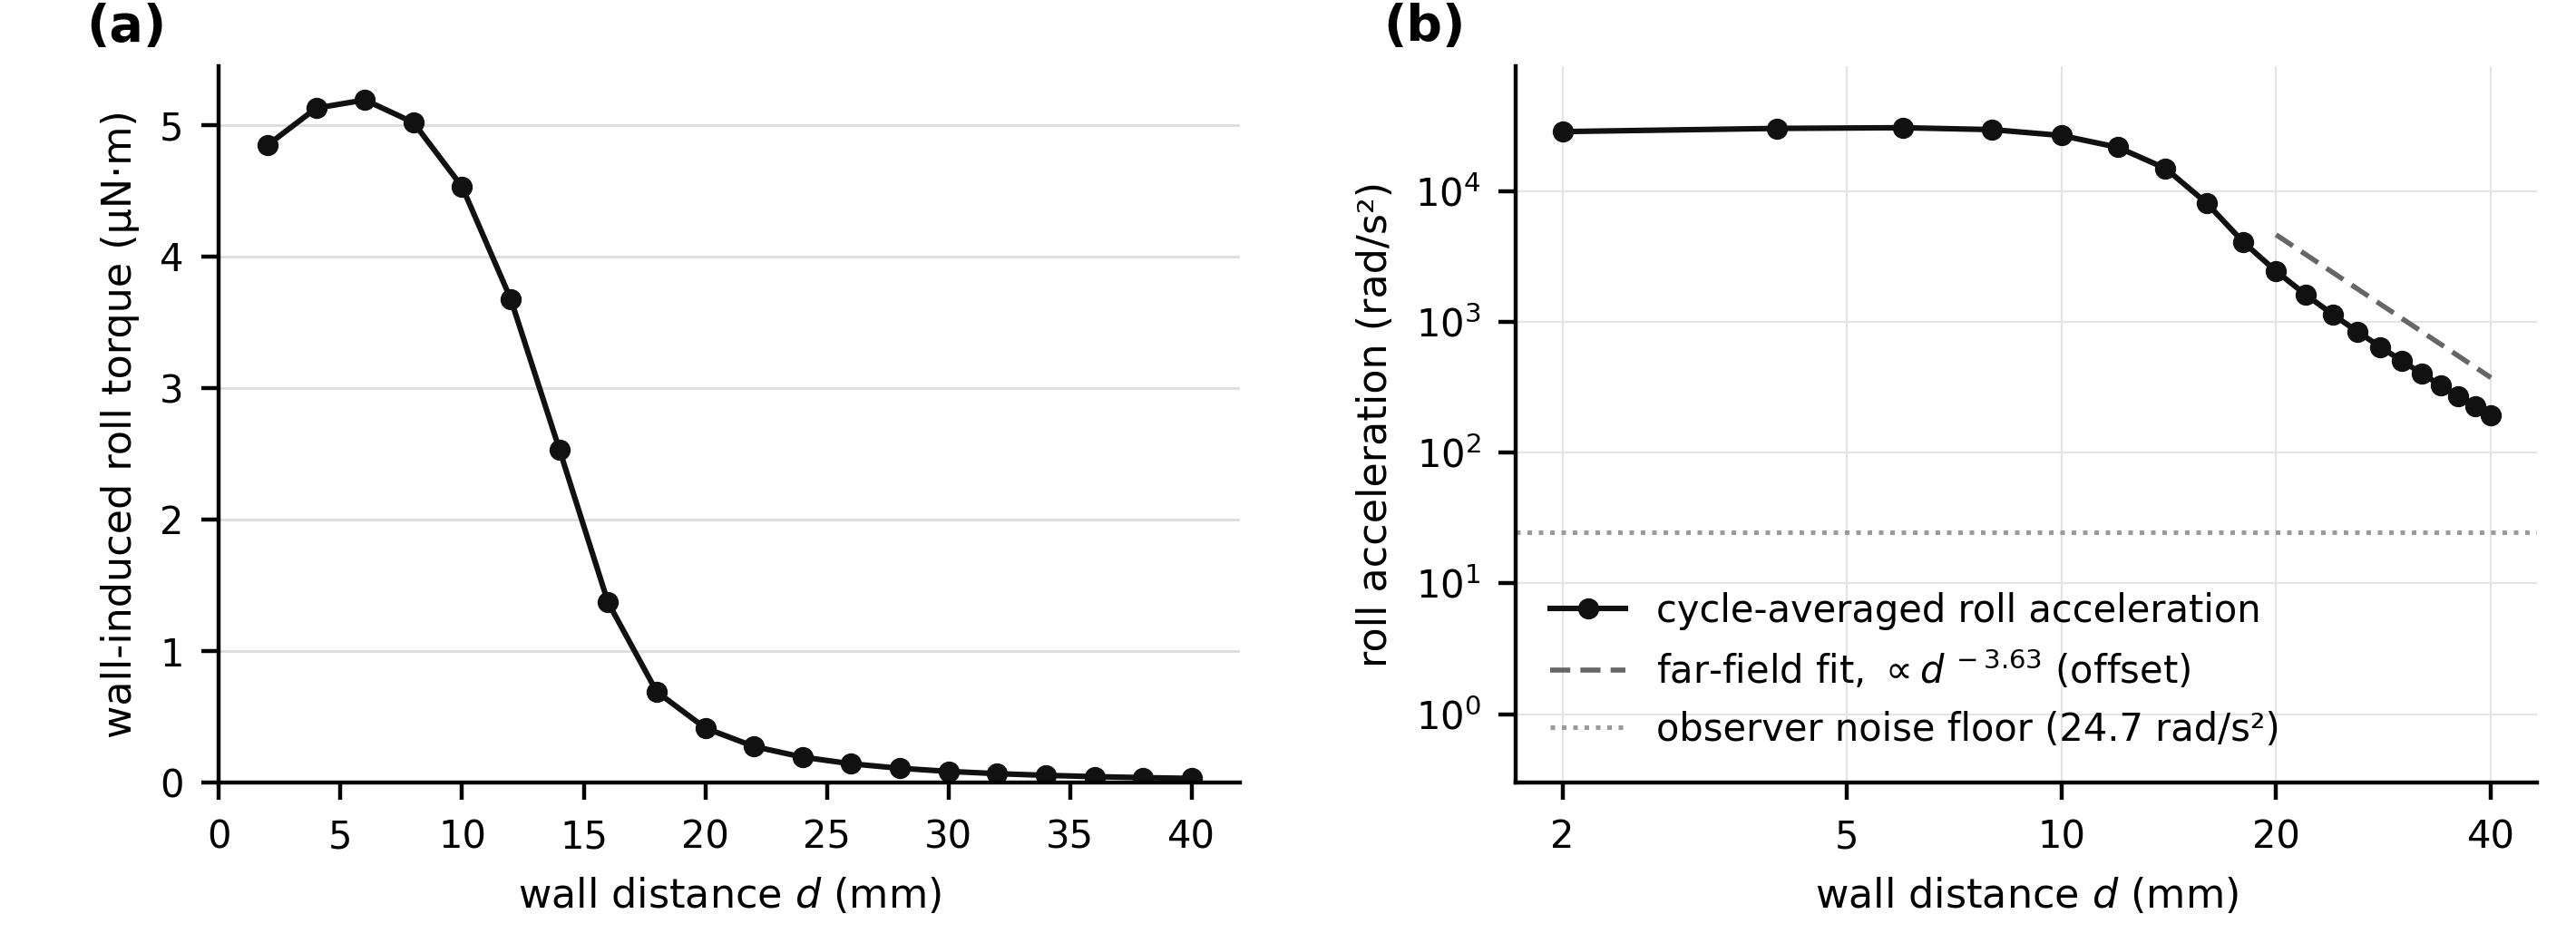
\includegraphics[width=0.9\linewidth]{figures/fig04_wingwash_signal.png}
\caption{Static response of the wing-wash signal to a single wall: (a) roll torque and (b) roll acceleration with far-field fit and noise floor.}
\label{fig:signal}
\end{figure*}

\begin{table}[t]
\centering
\caption{Power-law fits of the roll-acceleration decay over distance sub-intervals.}
\label{tab:falloff}
\footnotesize\setlength{\tabcolsep}{3pt}
\begin{tabular*}{\columnwidth}{@{\extracolsep{\fill}}llll@{}}
\toprule
Regime & Range (mm) & Exponent & $R^2$ \\
\midrule
Full band & 8 to 40 & $-3.59$ & $0.974$ \\
Past knee & 10 to 40 & $-3.90$ & $0.990$ \\
Near shoulder & 10 to 18 & $-3.16$ & $0.914$ \\
Far field & 20 to 40 & $-3.63$ & $0.998$ \\
\bottomrule
\end{tabular*}
\end{table}

Second, the resolution. In hover under nominal sensor noise, away from any wall, the filtered estimate fluctuates with a standard deviation of $24.7$~rad\,s$^{-2}$ about a mean indistinguishable from zero. Dividing this noise floor by the local slope of the static response gives the distance resolution, which is below one millimetre out to about $36$~mm and about $1.2$~mm at $38$~mm. It is finest, at approximately $7$ to $13~\mu$m, in the $10$ to $16$~mm region where the response is steepest; that region straddles the strike radius, and within the flyable band the finest values are $7$ to $9~\mu$m at $14$ to $16$~mm, coarsening to about $40~\mu$m at $20$~mm and $0.4$~mm at $30$~mm. This figure is a noise-equivalent distance under the assumed noise model, not a hardware resolution. Third, the observer fidelity. Comparing the settled estimate with the true induced acceleration, the observer recovers the signal with a direct-current gain of approximately $0.57$, essentially invariant with distance over the $15$ to $30$~mm range; below about $15$~mm the measurement is unreliable owing to position-hold drift. A step change in wall distance produces a ten-to-ninety-percent rise in about $13$~ms. Fourth, the two-wall response. Between two walls the induced roll acceleration is odd-symmetric in lateral offset and nulls at the corridor centreline; at offsets of $4$, $8$, and $12$~mm the directly measured two-wall response equals the difference of the single-wall response to a ratio of unity to within $2\times10^{-15}$. Figure~\ref{fig:observer_twowall} illustrates the last two properties. Panel (a) shows the observer gain against wall distance, which stays between $0.53$ and $0.59$ over the $15$ to $30$~mm band, and panel (b) shows the odd-symmetric two-wall response, which crosses zero at the centreline with a slope of about $109$~rad\,s$^{-2}$ per millimetre and coincides with the single-wall superposition.

\begin{figure*}[t]
\centering
\begin{subfigure}[b]{0.48\linewidth}
\centering
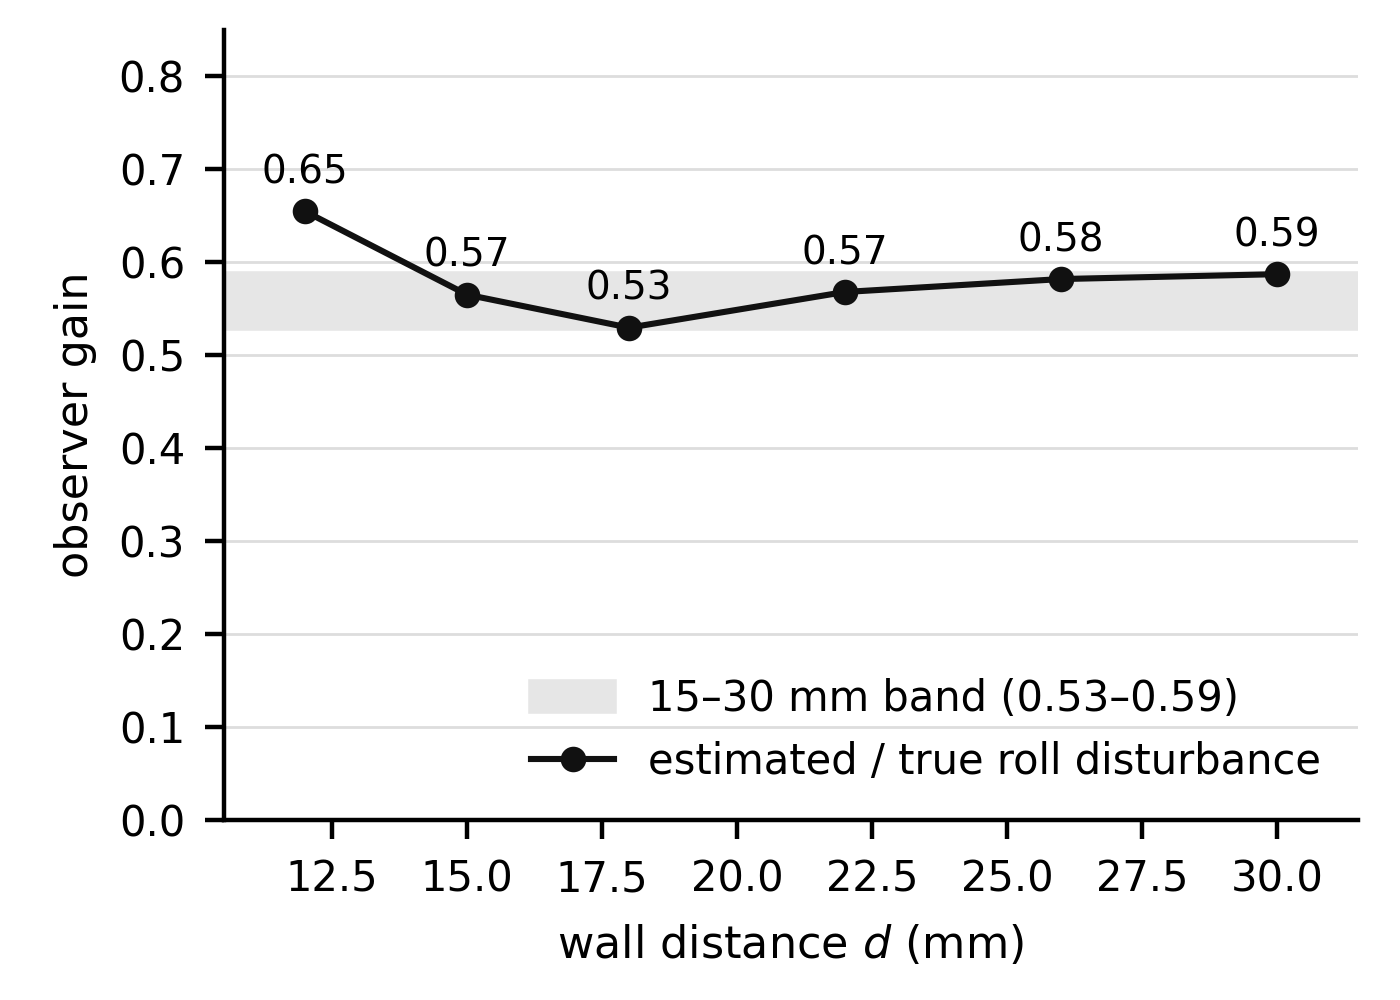
\includegraphics[width=\linewidth]{figures/fig06_observer_gain.png}
\caption{}
\end{subfigure}\hfill
\begin{subfigure}[b]{0.48\linewidth}
\centering
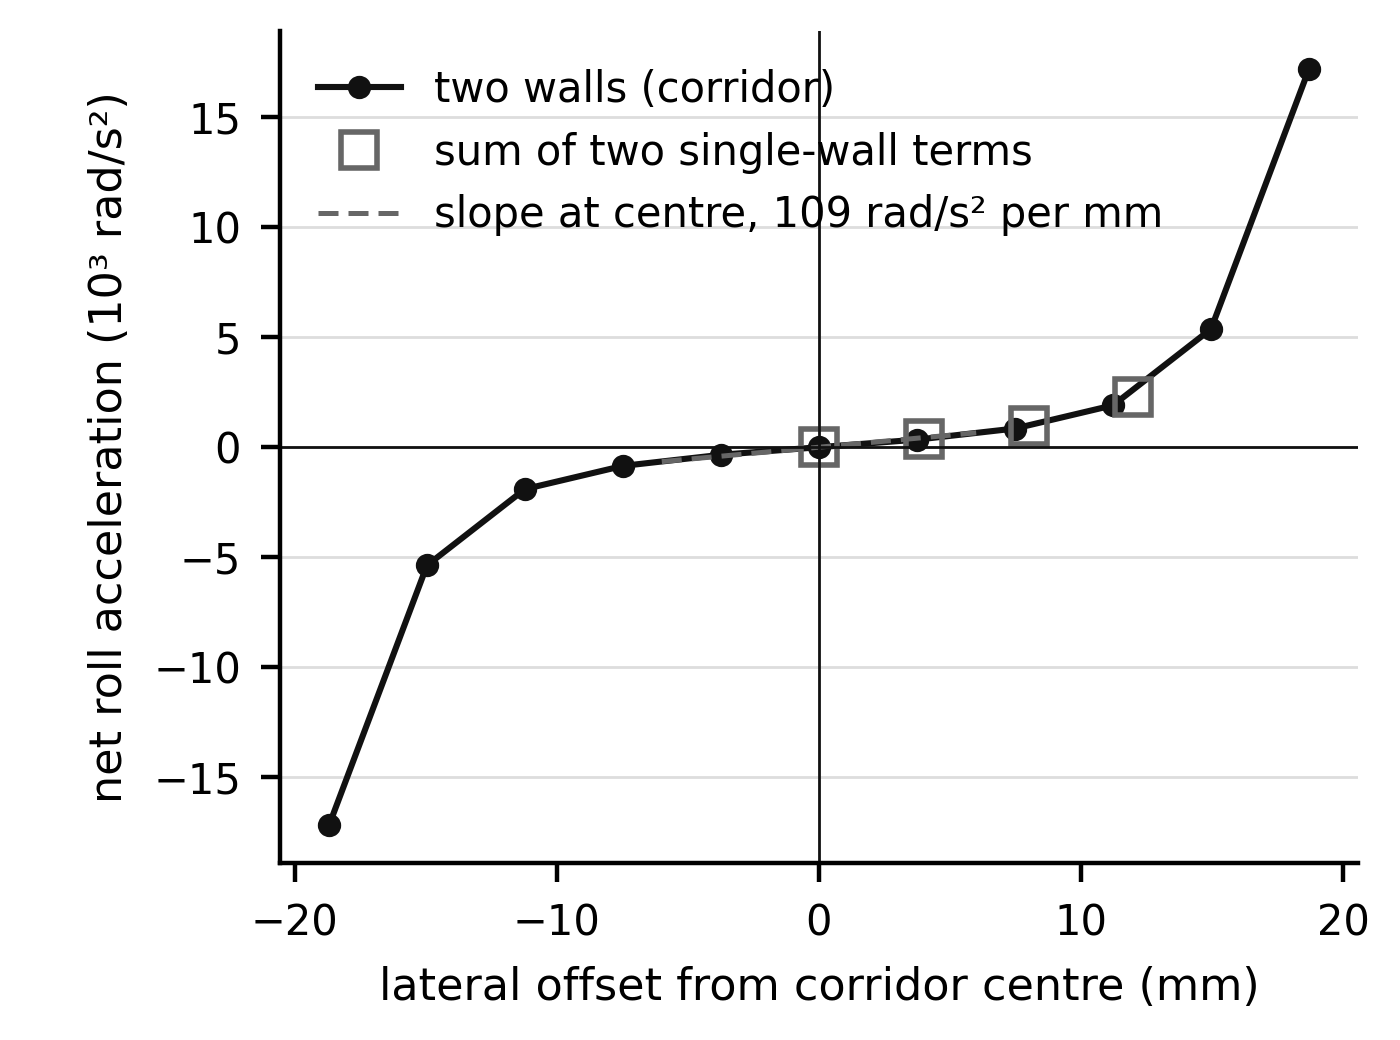
\includegraphics[width=\linewidth]{figures/fig05_two_wall_centering.png}
\caption{}
\end{subfigure}
\caption{Observer fidelity and two-wall response: (a) ratio of estimated to true roll disturbance and (b) net roll acceleration against lateral offset in a corridor.}
\label{fig:observer_twowall}
\end{figure*}

These properties do not all carry the same evidential weight, and Table~\ref{tab:evidence} classifies each by the four categories set out in Section~\ref{sec:aims}. A property is \emph{assumed} if it is a modelling choice, \emph{implied} if it follows from those choices without any flight being simulated, \emph{verified} if it is a check that the implementation reproduces what the model implies, and \emph{emergent} if it arises only from the closed-loop simulation and could not have been read off the model. Only the emergent properties are findings of the simulation; the assumed and implied ones would change with the modelling choices, and none of the four categories amounts to a physical measurement.

\begin{table}[t]
\centering
\caption{Evidential status of the reported properties of the wing-wash signal.}
\label{tab:evidence}
\footnotesize\setlength{\tabcolsep}{3pt}
\begin{tabularx}{\columnwidth}{@{}L{2.55cm}L{1.25cm}Y@{}}
\toprule
Property & Status & Basis \\
\midrule
Near-wall law, $K_{\mathrm{GE}}$, and cap $\kappa_{\max}$ & Assumed & Imposed by Eq.~\eqref{eq:kappa}, not derived from a flow solution \\
Sensor noise levels & Assumed & Eq.~\eqref{eq:noise} and Table~\ref{tab:noise} \\
Idealized feeler range readings & Assumed & Exact ray-cast range with additive noise \\
Side-resolving sign of the roll torque & Implied & The near wing is enhanced more than the far wing, Eq.~\eqref{eq:tauwall} \\
Saturation knee below about $6$~mm & Implied & Consequence of the cap $\kappa_{\max}$, not a resolved flow regime \\
Decay exponents of Table~\ref{tab:falloff} & Implied & Computed from the law, the wing geometry, and the stroke; noise plays no part \\
Two-wall odd symmetry and centreline null & Implied & Wall contributions add strip by strip in the model \\
Two-wall superposition, ratio of unity & Verified & Implementation check of the additive form, not an aerodynamic result \\
Noise floor and distance resolution & Emergent & Closed-loop hover under the assumed noise; a noise-equivalent distance \\
Resolvable band of $8$ to $40$~mm & Emergent & Implied response set against the emergent noise floor \\
Observer gain of $0.57$ and $13$~ms rise & Emergent & Observer and plant dynamics in closed loop \\
Detection, navigation, and ablation outcomes & Emergent & Closed-loop flights of Sections~\ref{sec:results_detection} to~\ref{sec:results_width} \\
\bottomrule
\end{tabularx}
\end{table}

\subsection{Detection Floor, Localization, and Sizing}
\label{sec:results_detection}

The elementary detection limit was measured by placing a single opening of controlled length in one wall of a $64$~mm corridor and sweeping its length, with five noise realizations at each length under nominal sensor noise. The outcomes are given in Table~\ref{tab:detection}. The opening was detected in all five realizations at every length from $12$ to $60$~mm and in none at $10$~mm, so the detection floor lies between $10$ and $12$~mm. Mean localization error of the estimated opening midpoint was below one millimetre for openings up to $35$~mm, with a largest single-flight error of $1.7$~mm, and rose to between $2$ and $4$~mm for openings of $40$ to $60$~mm. The raw length estimate is biased short, and a single linear calibration fitted to the fully detected lengths (slope $0.884$, offset $-7.98$~mm) recovered the true length with a per-flight root-mean-square residual of $0.98$~mm over $12$ to $40$~mm and $1.05$~mm over $12$ to $60$~mm; because the calibration is fitted to these same flights, the residuals are in-sample. The $80$~mm opening marks the upper limit of the procedure: three of the five flights there did not complete the corridor, one of them logging no opening and two logging a truncated one, while the two flights that did complete sized the opening to within $1.5$~mm.

\begin{table}[t]
\centering
\caption{Detection rate, localization error, and calibrated size error versus opening length.}
\label{tab:detection}
\footnotesize\setlength{\tabcolsep}{3pt}
\begin{threeparttable}
\begin{tabular*}{\columnwidth}{@{\extracolsep{\fill}}llll@{}}
\toprule
True length (mm) & Detection & Loc. error (mm) & Size error (mm) \\
\midrule
10 & 0/5 & n/a & n/a \\
12 & 5/5 & 0.72 & $-0.98$ \\
15 & 5/5 & 0.59 & $-0.04$ \\
18 & 5/5 & 0.49 & $-0.66$ \\
20 & 5/5 & 0.36 & $+0.30$ \\
25 & 5/5 & 0.61 & $+0.47$ \\
30 & 5/5 & 0.58 & $+0.54$ \\
35 & 5/5 & 0.96 & $+1.75$ \\
40 & 5/5 & 2.03 & $-0.05$ \\
50 & 5/5 & 3.83 & $-1.10$ \\
60 & 5/5 & 3.74 & $-0.24$ \\
80\tnote{a} & 4/5 & 7.29 & $-19.0$ \\
\bottomrule
\end{tabular*}
\begin{tablenotes}\footnotesize
\item[a] Three of the five flights at $80$~mm did not complete the corridor, and this length is excluded from the calibration fit; the two completed flights give errors of $2.8$ and $4.1$~mm in location and $-1.3$ and $-1.5$~mm in size.
\end{tablenotes}
\end{threeparttable}
\end{table}

\subsection{Randomized-Course Inspection}
\label{sec:results_batch}

Before the randomized ensemble, the integrated system was flown on a crafted three-leg course containing three wall openings, and Figure~\ref{fig:mission} shows the resulting flight. The vehicle centred itself in each leg, negotiated both corners, and reached the goal in $17.2$~s with a minimum clearance of $21.6$~mm, logging all three openings on the correct wall.

\begin{figure}[t]
\centering
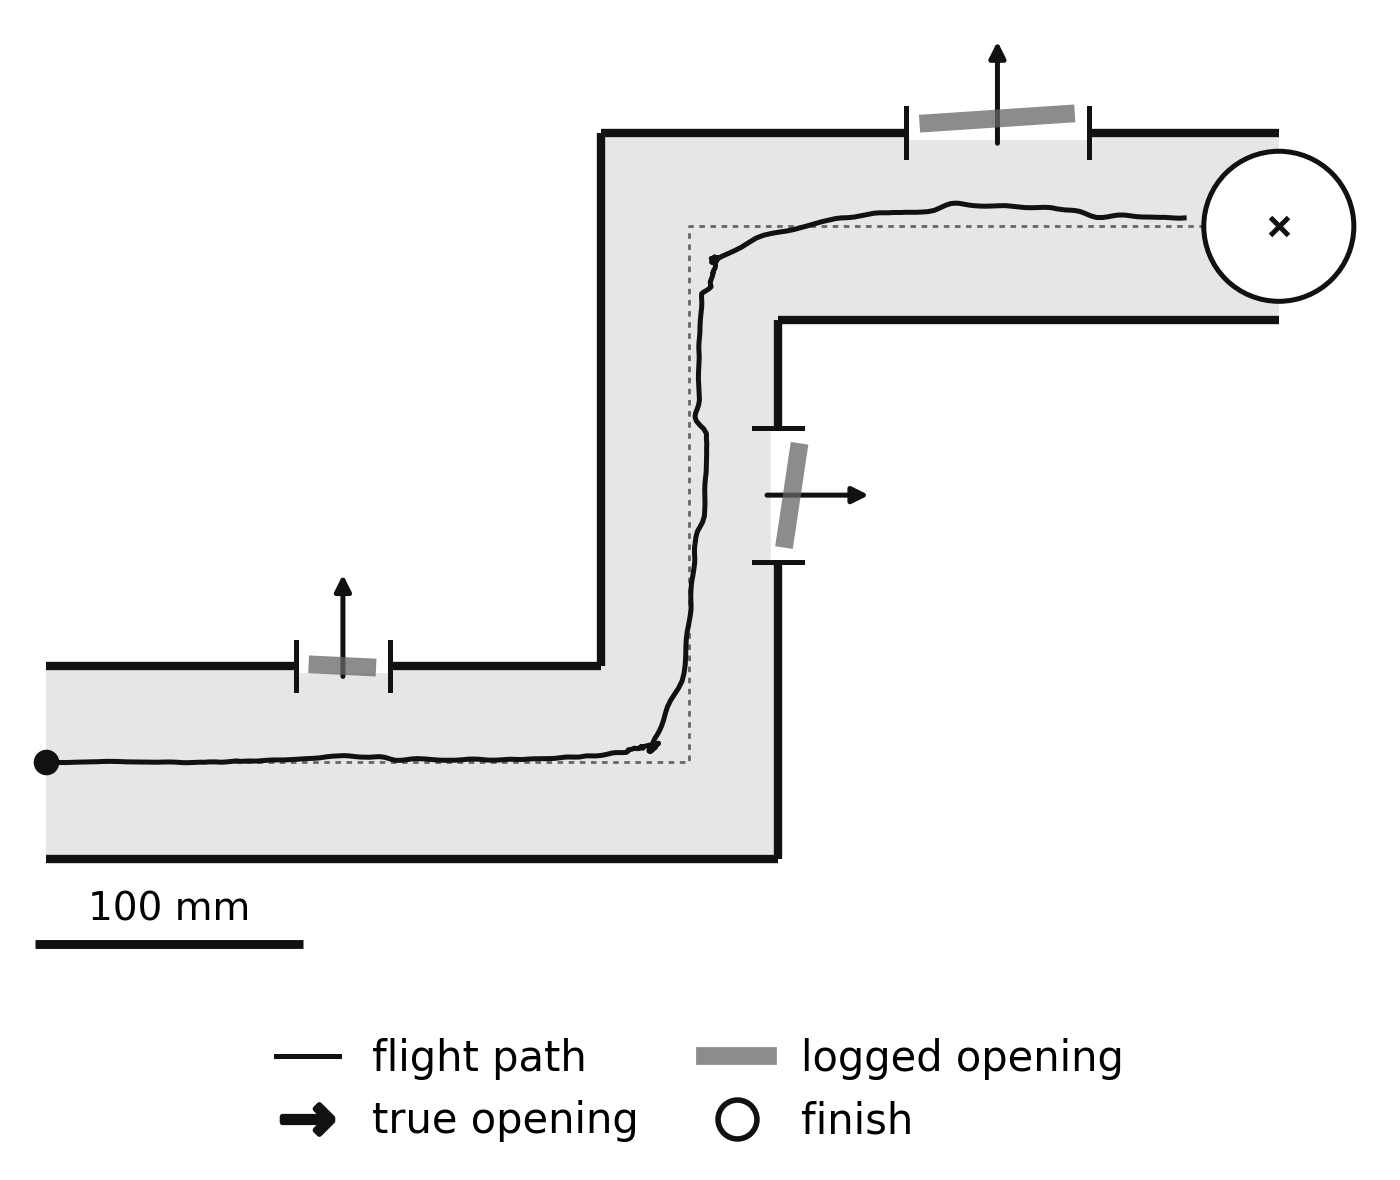
\includegraphics[width=\linewidth]{figures/fig09_example_mission.png}
\caption{Example flight on a crafted three-leg course with true and logged wall openings.}
\label{fig:mission}
\end{figure}

The integrated system was then evaluated across a primary ensemble of $40$ independently generated multi-turn courses, each flown once under nominal noise, with the aerodynamic and tactile channels both active. The vehicle reached the goal on $35$ of the $40$ courses. Of these, five reached the goal having incurred a wall strike along the way, so the strike-free completion rate was $30$ of $40$. Of the openings present, $43$ were detected out of the $58$ in completed courses, which is $74$ percent conditionally and $43$ of $68$, or $63$ percent, over all generated courses. The mean localization error of detected openings was $7.9$~mm, with a median of $6.9$~mm, and the system produced one false positive across the $35$ completed courses. Of the $43$ matched detections, $40$ lay within $20$~mm of the true midpoint and the remaining three at $23.7$, $28.9$, and $38.2$~mm, so the detection count would be unchanged under any match tolerance from $39$~mm up to the $60$~mm used, and would be $40$ of $58$ under a tolerance of $20$~mm. These figures are summarized in Table~\ref{tab:batch}.

\begin{table}[t]
\centering
\caption{Randomized-course inspection outcomes on the primary ensemble.}
\label{tab:batch}
\footnotesize\setlength{\tabcolsep}{3pt}
\begin{tabular*}{\columnwidth}{@{\extracolsep{\fill}}lll@{}}
\toprule
Metric & Conditional & End-to-end \\
\midrule
Courses generated & -- & 40 \\
Reached goal & -- & 35/40 (88\%) \\
Reached goal, strike-free & -- & 30/40 (75\%) \\
Per-passage detection & 30/35 (86\%) & 30/40 (75\%) \\
Per-opening detection & 43/58 (74\%) & 43/68 (63\%) \\
Localization error (mm) & $7.9$ (mean), $6.9$ (median) & -- \\
False positives per course & 0.03 (1 in 35) & 0.025 (1 in 40) \\
\bottomrule
\end{tabular*}
\end{table}

\subsection{Channel Ablation}
\label{sec:results_ablation}

The contribution of each sensing channel was measured by removing it on the identical primary ensemble, with all other factors held fixed. Table~\ref{tab:ablation} reports goal-reaching and detection for the four configurations, and Figure~\ref{fig:abl_bars} shows them. In the no-feelers configuration the feeler-based steering, wall-avoidance, and opening-detection terms are removed, but the forward ray is retained for the speed law and the corner-turn trigger, so lateral centring rests on the aerodynamic channel while the vehicle can still slow and turn at a corner; this configuration is therefore not the aerodynamic channel acting entirely alone. Removing the feelers in this sense reduced goal-reaching from $35$ to $16$ of $40$ and produced no logged detections, since disabling the feelers also disables the opening logger. Removing all environmental sensing (open-loop) produced no goal-reaching. Removing the aerodynamic channel while retaining the feelers produced $32$ of $40$ goal-reaching, against $35$ for the full configuration, with detection of a comparable number of openings.

\begin{table}[t]
\centering
\begin{threeparttable}
\caption{Ablation outcomes across the four sensing configurations.}
\label{tab:ablation}
\footnotesize\setlength{\tabcolsep}{3pt}
\begin{tabular*}{\columnwidth}{@{\extracolsep{\fill}}lllll@{}}
\toprule
Configuration & Reached & Strike-free & Per-opening & FP/course \\
\midrule
Full & 35/40 & 30/40 & 43/58 & 0.03 \\
No wing-wash & 32/40 & 29/40 & 41/54 & 0.03 \\
No feelers & 16/40 & 15/40 & 0/25\tnote{a} & 0.00 \\
Open-loop & 0/40 & 0/40 & -- & -- \\
\bottomrule
\end{tabular*}
\begin{tablenotes}\footnotesize
\item[a] The zero detection without feelers is structural, since the opening logger is disabled with the feeler channel, and is not an observed detection miss.
\end{tablenotes}
\end{threeparttable}
\end{table}

\begin{figure}[t]
    \centering
    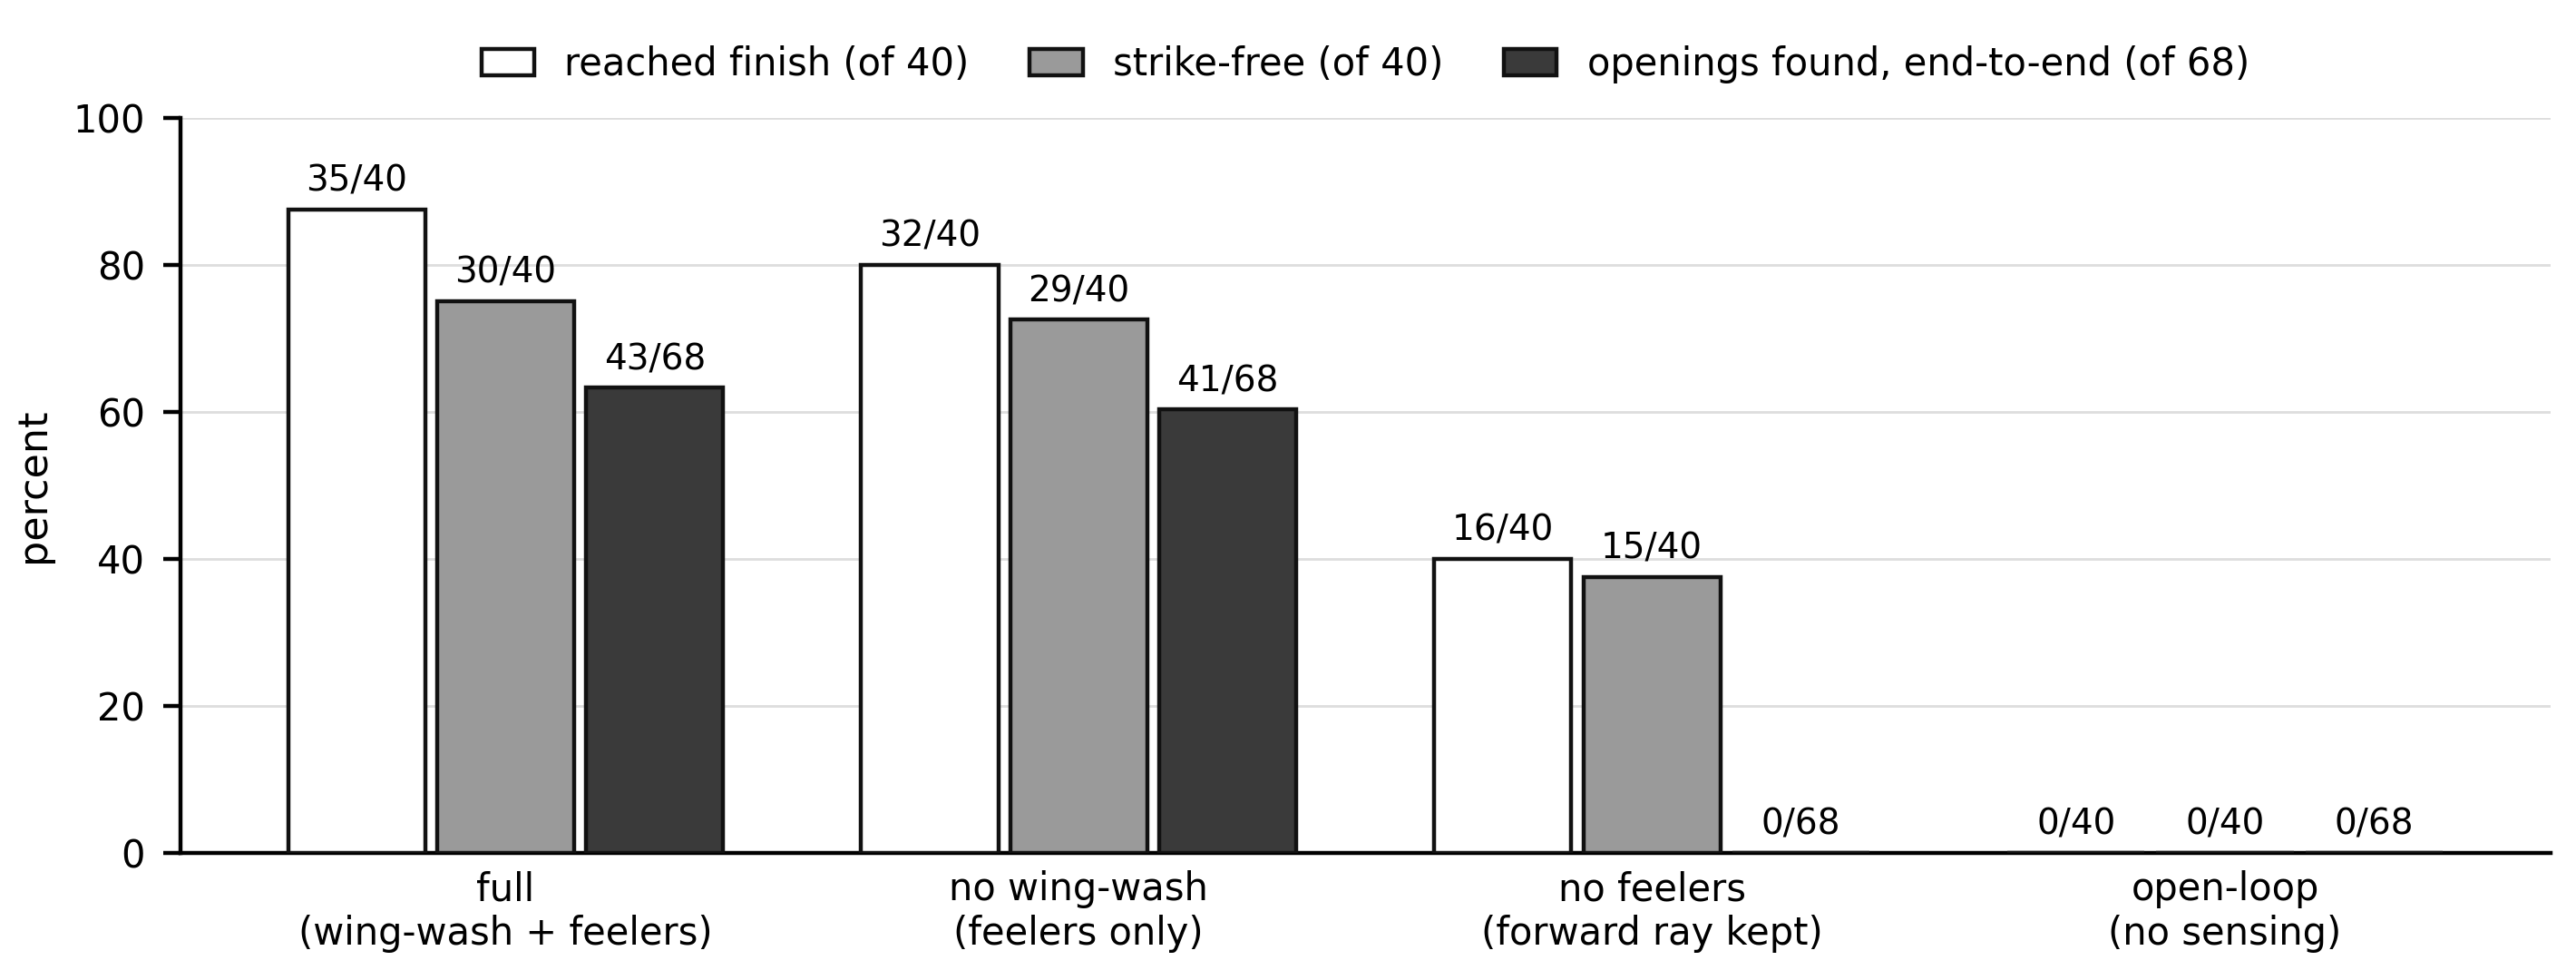
\includegraphics[width=\linewidth]{figures/fig10_ablation_truewall.png}
    \caption{Goal-reaching, strike-free completion, and end-to-end opening detection for the four sensing configurations.}
    \label{fig:abl_bars}
\end{figure}

The clearance statistics of the full and no-wing-wash configurations are compared in Figure~\ref{fig:abl_clear}, which shows the per-flight minimum clearance over the paired-seed flights of Section~\ref{sec:results_stats} against the wingtip-strike radius. In the single-seed ablation flights of Table~\ref{tab:ablation}, the mean minimum clearance was $18.3$~mm for the full configuration and $17.4$~mm without the aerodynamic channel, the worst single clearance was $2.2$~mm and $1.6$~mm respectively, and the two configurations incurred wall strikes on seven and eight courses.

\begin{figure}[t]
    \centering
    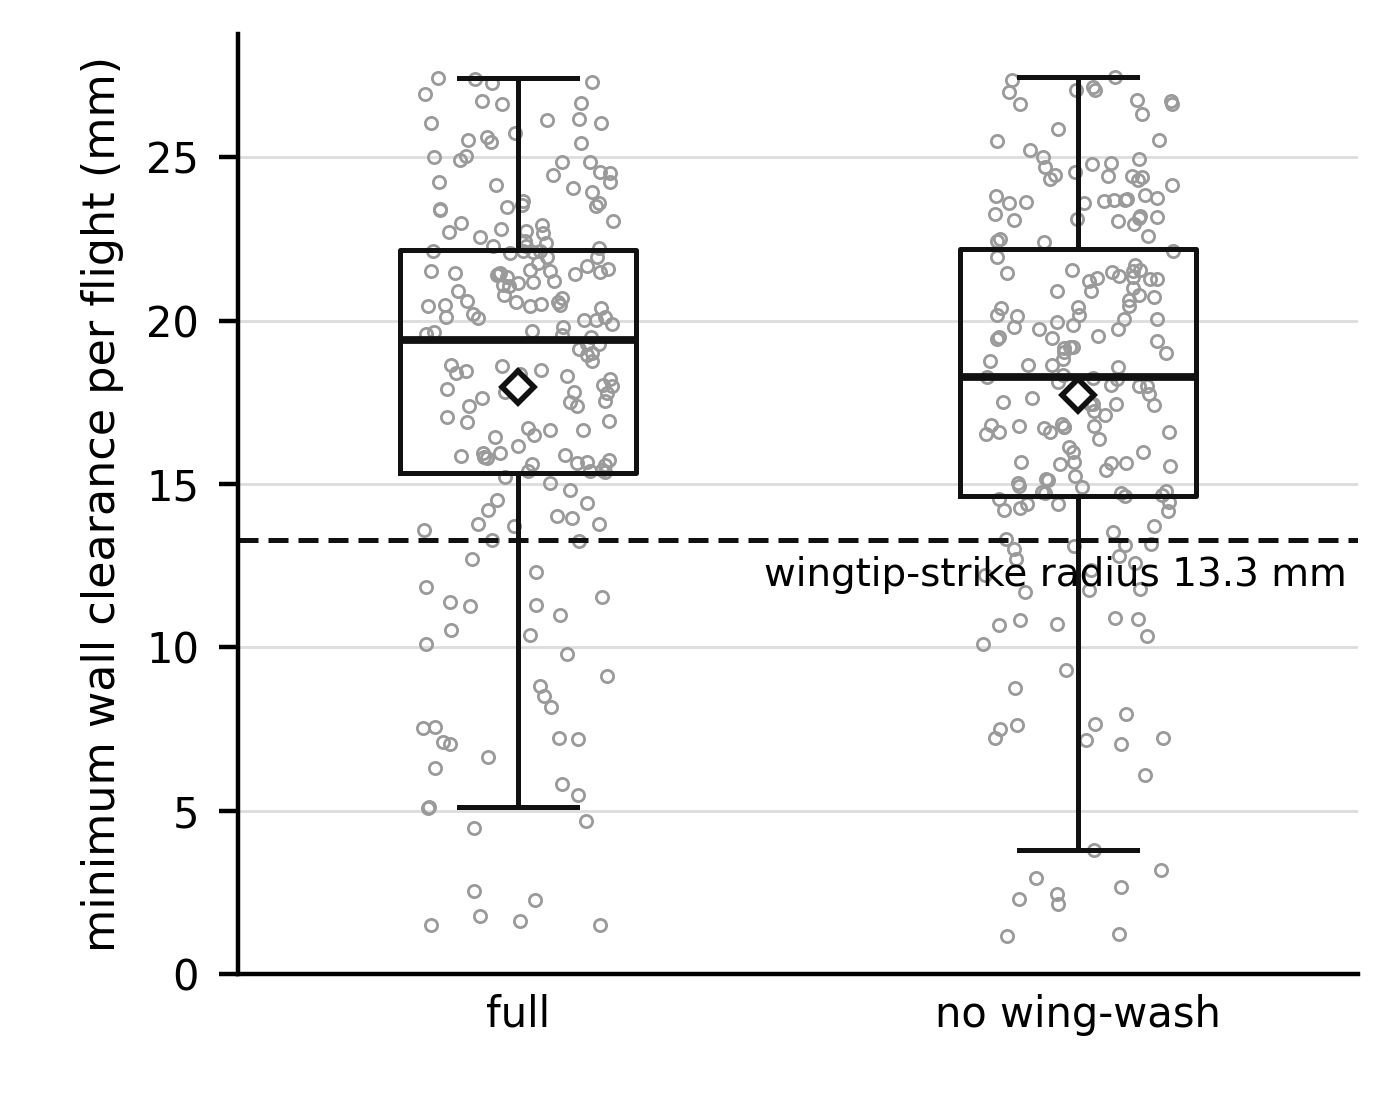
\includegraphics[width=\linewidth]{figures/fig13_clearance_truewall.png}
    \caption{Per-flight minimum clearance for the full and no-wing-wash configurations across the $200$ paired-seed flights of each configuration.}
    \label{fig:abl_clear}
\end{figure}

\subsection{Statistical Comparison of the Aerodynamic Channel}
\label{sec:results_stats}

The central comparison, between the full configuration and the configuration with the aerodynamic channel removed, was analysed under the pre-specified paired design of Section~\ref{sec:method_stats}, using five matched noise seeds per course across the primary ensemble, for $200$ paired trials. Table~\ref{tab:stats} reports the results. The paired difference in strike-free completion was $+1.0$ percentage points in favour of the full configuration, with a $95$ percent confidence interval of $[-5.0, +6.5]$ percentage points and an exact McNemar $p$-value of $0.83$. Per-opening detection on jointly completed trials differed by $+1.1$ percentage points, and mean minimum clearance by $+0.24$~mm, both with confidence intervals spanning zero. The confidence interval on the primary metric crosses the pre-specified equivalence margin of $\pm 5$ percentage points at its upper end, so the comparison is classified as inconclusive with respect to formal equivalence at this sample size; no difference was resolved on any metric. The exception for clearance near the goal, described in Section~\ref{sec:method_stats}, affects two of the $400$ flights: two no-wing-wash flights on one course completed with minimum clearances of $8.0$ and $8.8$~mm inside the $50$~mm goal zone and are scored as strike-free. Counting them as strikes gives $152$ against $148$ of $200$, a paired difference of $+2.0$ percentage points with an interval of $[-3.5, +7.5]$ and a McNemar $p$-value of $0.50$, which leaves the classification unchanged. Rescoring without the exception and with the full $13.6$~mm wingtip reach as the strike radius gives $151$ against $148$, a difference of $+1.5$ percentage points with an interval of $[-4.0, +6.5]$, again unchanged. No completed flight of the single-seed primary ensemble or of the confirmatory test of Section~\ref{sec:results_confirm} is affected by the exception.

\begin{table}[t]
\centering
\caption{Paired comparison of the full and no-wing-wash configurations.}
\label{tab:stats}
\footnotesize\setlength{\tabcolsep}{3pt}
\begin{tabular*}{\columnwidth}{@{\extracolsep{\fill}}lll@{}}
\toprule
Metric & Paired diff. & 95\% CI \\
\midrule
Strike-free completion & $+1.0$ pp & $[-5.0, +6.5]$ pp \\
Per-opening detection & $+1.1$ pp & $[-1.2, +3.5]$ pp \\
Mean min-clearance & $+0.24$ mm & $[-0.57, +0.98]$ mm \\
\bottomrule
\end{tabular*}
\end{table}

\subsection{Search for a Regime of Advantage}
\label{sec:results_regimes}

Two further analyses tested whether an operating regime exists in which the aerodynamic channel confers a measurable advantage. The first swept the number of legs from two to six, on fresh noise seeds, comparing the two configurations on strike-free completion. A difference observed on the uncorrected harness, $48$ against $34$ of $100$ with a McNemar $p$-value of $0.0125$, did not reproduce on the corrected harness with fresh seeds: pooled over the sweep, the full configuration completed $48$ of $100$ strike-free against $42$ of $100$ without the aerodynamic channel, with an exact McNemar $p$-value of $0.29$. The second analysis degraded the feelers by limiting their range from the nominal $0.16$~m down to $0.03$~m, comparing the two configurations at each level; the outcomes are shown in Figure~\ref{fig:feeler}. At the three widest limits the two configurations were indistinguishable. At a limit of $0.05$~m the full configuration completed $25$ of $40$ courses strike-free against $18$ of $40$ without the aerodynamic channel, a difference whose confidence interval nonetheless reaches zero and whose McNemar $p$-value is $0.118$. At a limit of $0.03$~m both configurations failed, completing zero and one of the paired courses respectively. This was the only condition of the sweep in which the aerodynamic channel showed an advantage. Because it was one unplanned cell among several and rested on a single noise seed per course, it was treated as hypothesis-generating and was tested separately, as reported in Section~\ref{sec:results_confirm}. The dropout and elevated-noise degradation axes were not evaluated. Table~\ref{tab:regimes} lists the strike-free outcome of every cell of both analyses, with the paired difference and the exact McNemar $p$-value for each.

\begin{table}[t]
\centering
\begin{threeparttable}
\caption{Strike-free completion of the full and no-wing-wash configurations in the leg-sweep and feeler-range analyses.}
\label{tab:regimes}
\footnotesize\setlength{\tabcolsep}{3pt}
\begin{tabular*}{\columnwidth}{@{\extracolsep{\fill}}lllll@{}}
\toprule
Condition & Full & No wing-wash & Diff. (pp) & $p$ \\
\midrule
\multicolumn{5}{@{}l}{\emph{Number of legs}} \\
2 & 13/20 & 12/20 & $+5$ & 1.000 \\
3 & 10/20 & 9/20 & $+5$ & 1.000 \\
4 & 6/20 & 7/20 & $-5$ & 1.000 \\
5 & 12/20 & 10/20 & $+10$ & 0.727 \\
6 & 7/20 & 4/20 & $+15$ & 0.375 \\
Pooled & 48/100 & 42/100 & $+6$ & 0.286 \\
\midrule
\multicolumn{5}{@{}l}{\emph{Feeler range limit}} \\
0.16 m (nominal)\tnote{a} & 32/40 & 32/40 & $0.0$ & 1.000 \\
0.12 m & 30/40 & 31/40 & $-2.5$ & 1.000 \\
0.08 m & 31/40 & 31/40 & $0.0$ & 1.000 \\
0.05 m & 25/40 & 18/40 & $+17.5$ & 0.118 \\
0.03 m\tnote{b} & 0/32 & 1/32 & $-3.1$ & 1.000 \\
\bottomrule
\end{tabular*}
\begin{tablenotes}\footnotesize
\item[a] The nominal row is the matching single-seed slice of the paired-seed runs of Section~\ref{sec:results_stats}, not a separate set of flights.
\item[b] Only $32$ of the $40$ courses were flown in both configurations at this limit.
\end{tablenotes}
\end{threeparttable}
\end{table}

\begin{figure}[t]
\centering
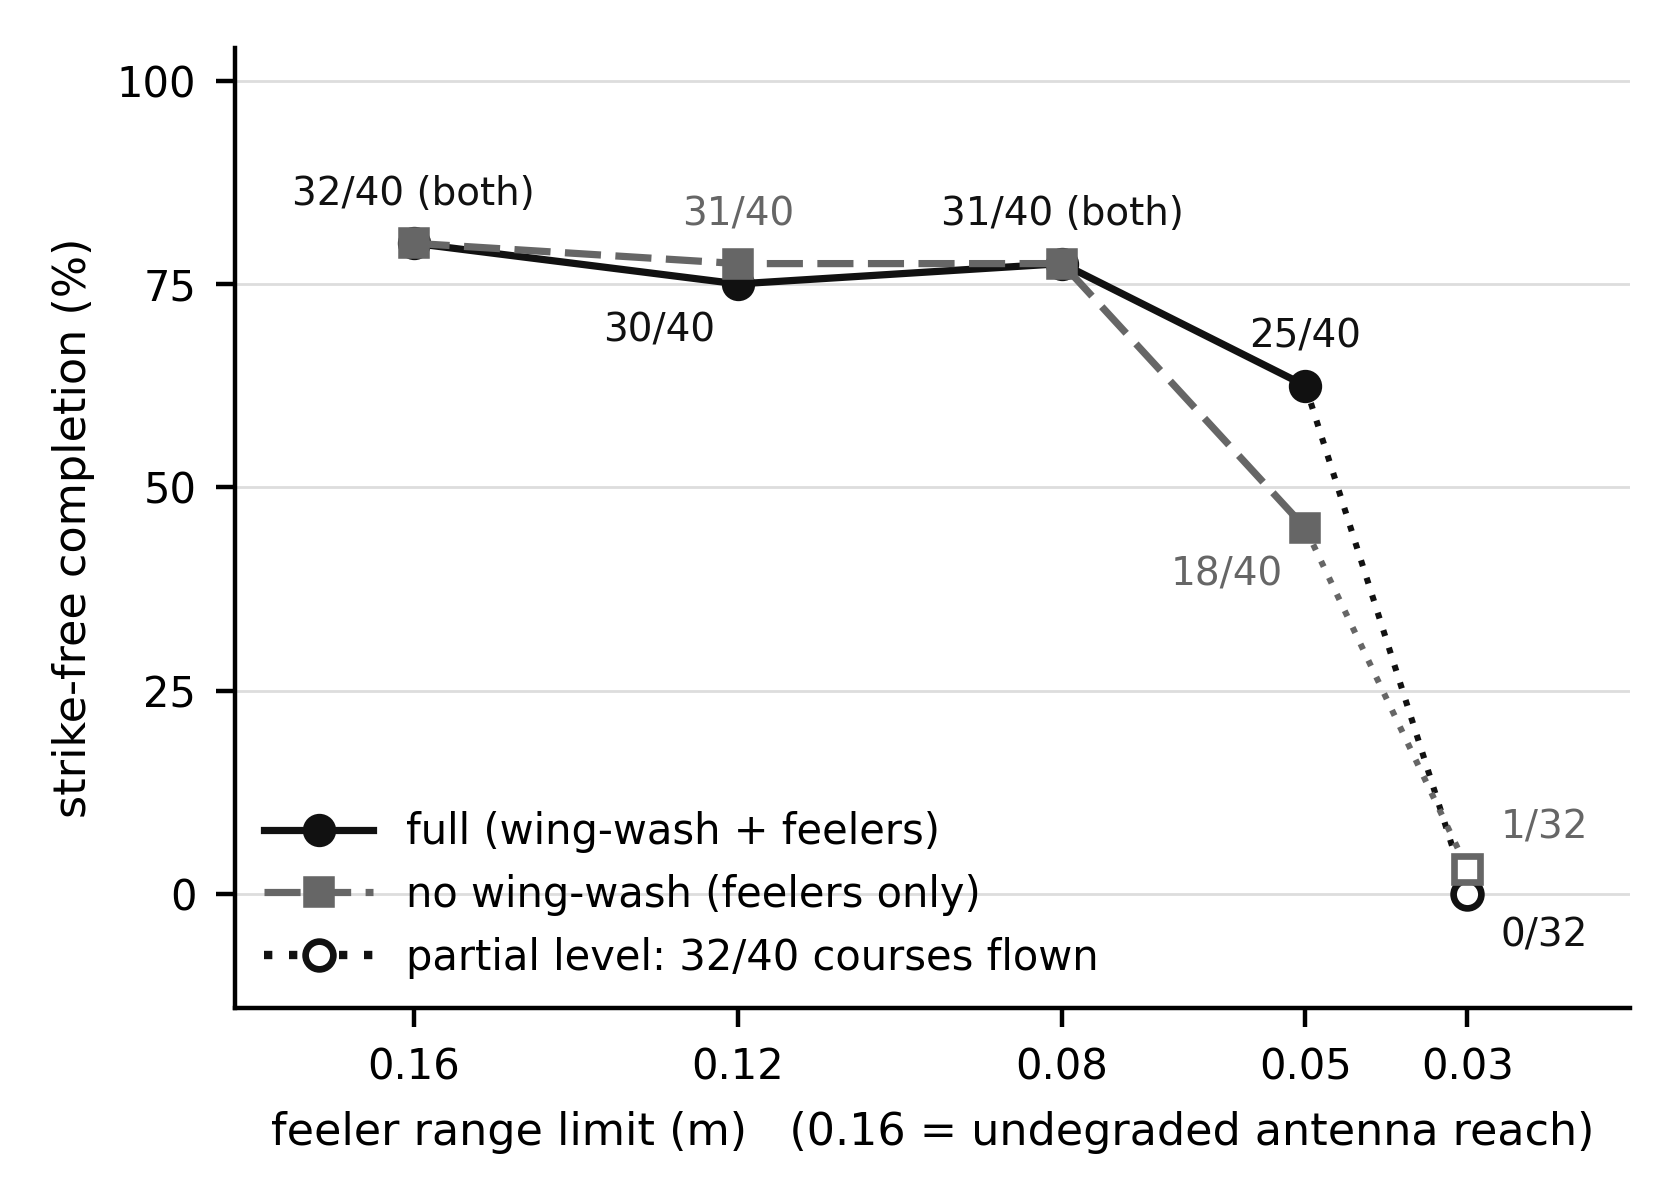
\includegraphics[width=\linewidth]{figures/design_c_feeler_range.png}
\caption{Strike-free completion under feeler range limitation.}
\label{fig:feeler}
\end{figure}

Figure~\ref{fig:paired} summarizes every paired comparison of the two configurations, giving the difference in strike-free completion with its $95$ percent confidence interval for the primary ensemble, the leg sweep, each feeler-range limit of the exploratory sweep, and the confirmatory test of Section~\ref{sec:results_confirm}, against the pre-specified $\pm 5$ percentage-point margin. Among the comparisons that preceded the confirmatory test no interval excludes zero, and the one point estimate well outside the margin, at a feeler range of $0.05$~m, comes from a cell that was not pre-specified and used a single seed per course. The interval of the confirmatory test lies wholly above both zero and the margin.

\begin{figure*}[t]
\centering
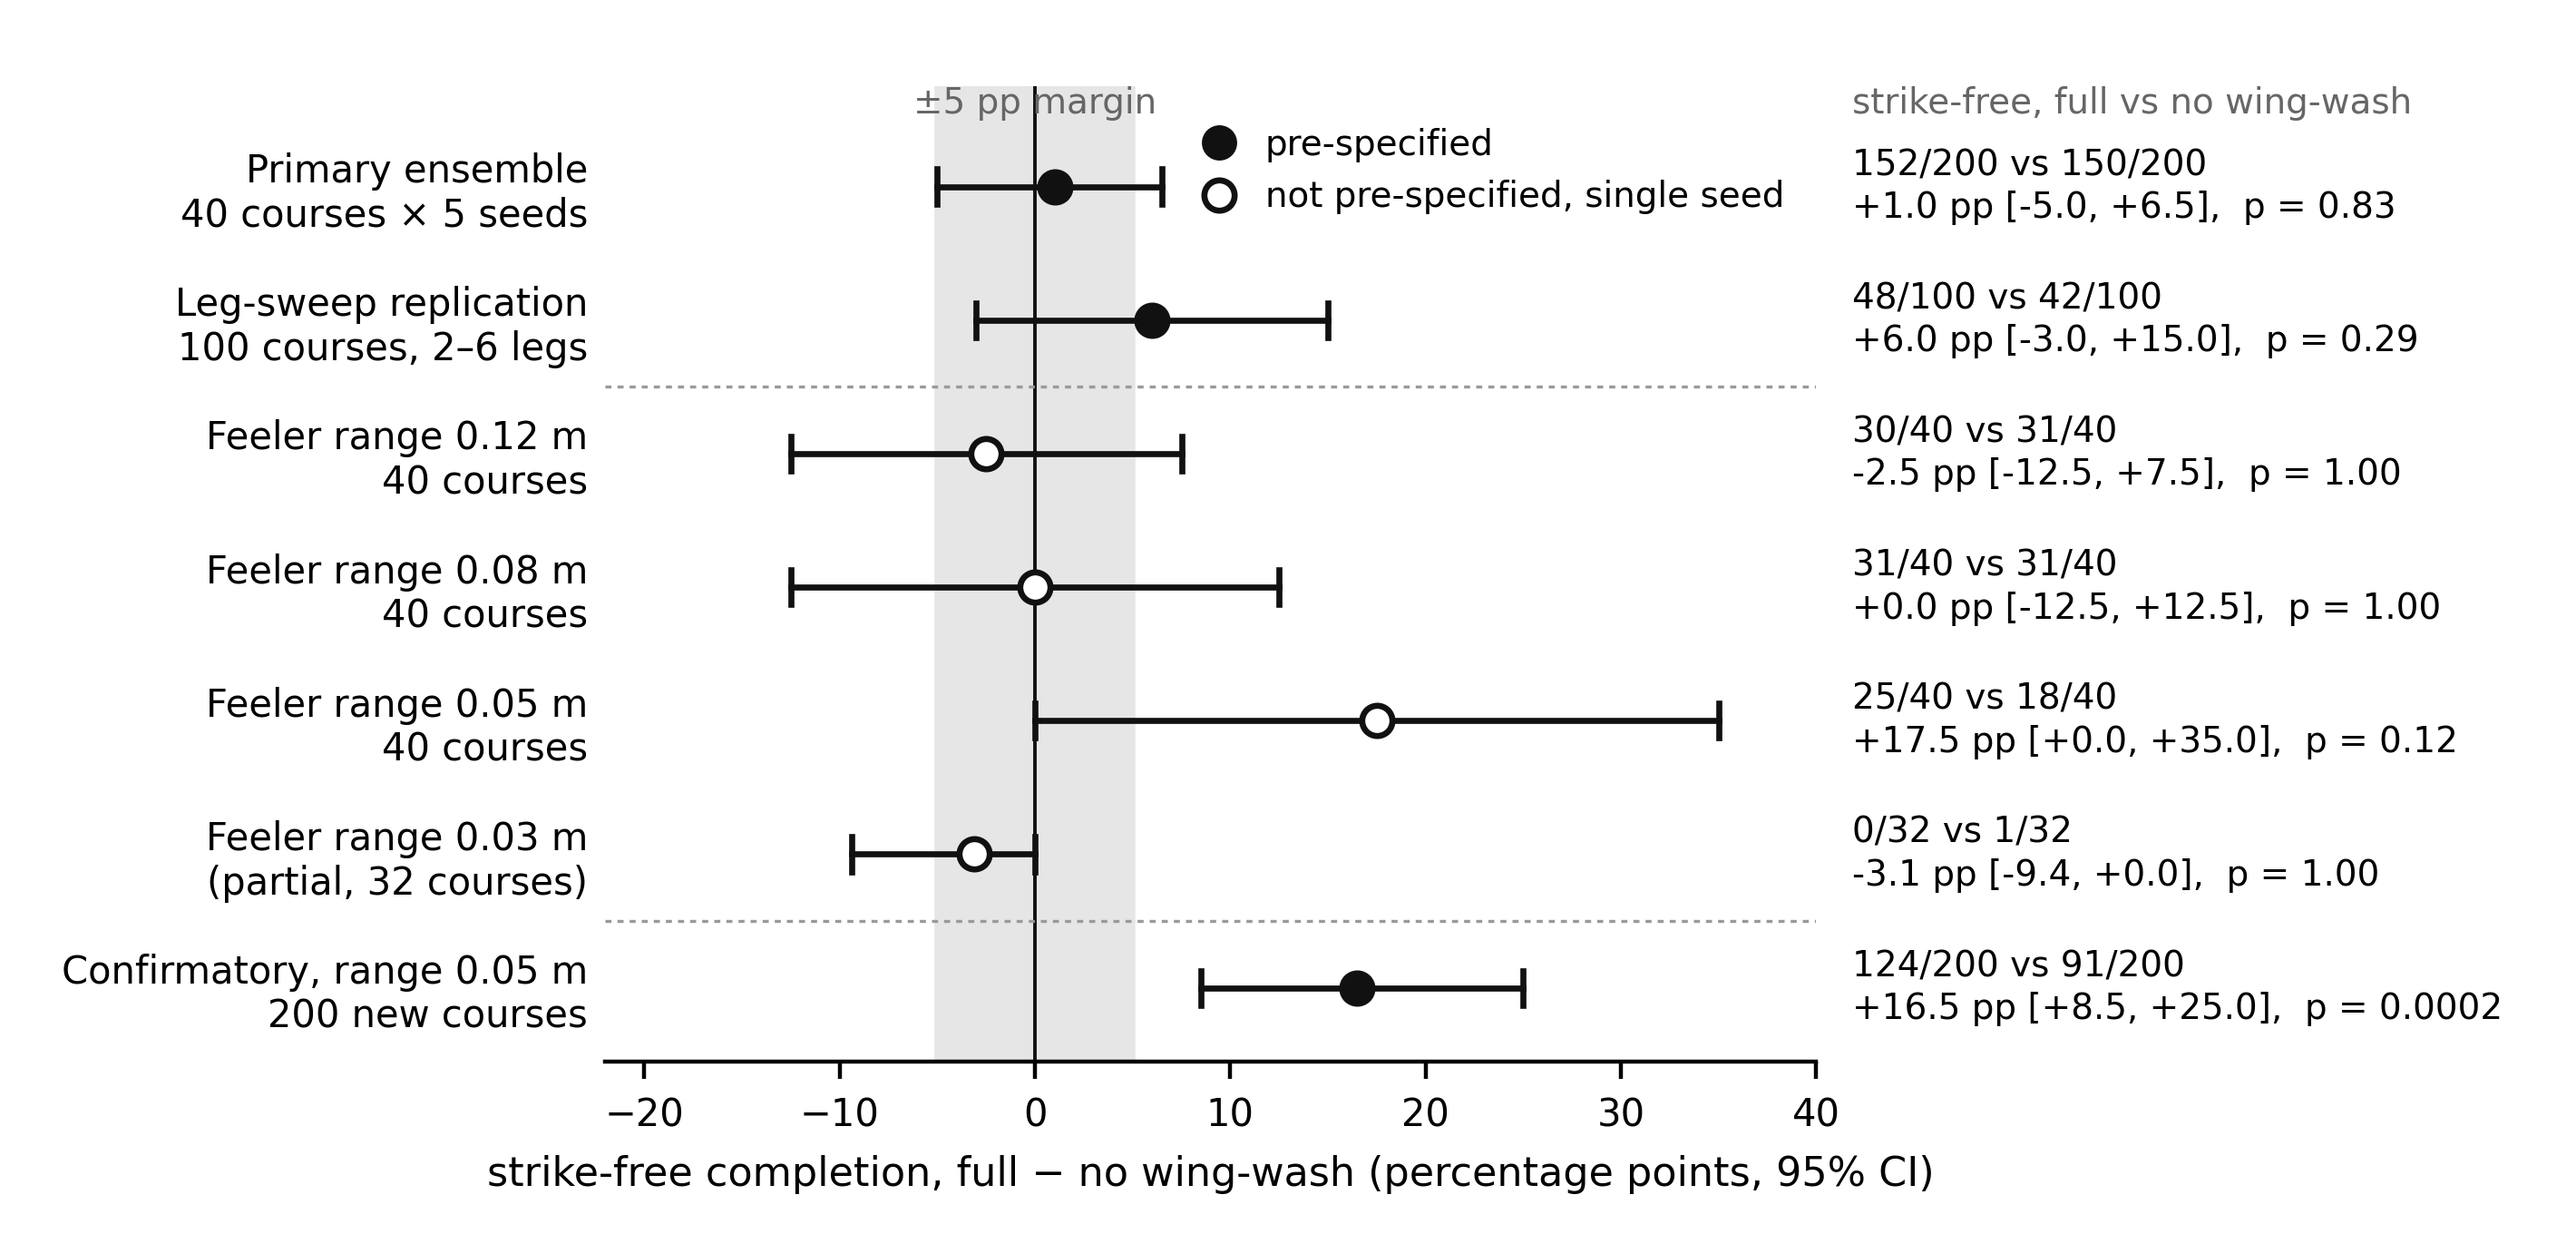
\includegraphics[width=0.9\linewidth]{figures/fig11_paired_differences.png}
\caption{Paired differences in strike-free completion (full minus no-wing-wash) with 95\% confidence intervals across all comparisons.}
\label{fig:paired}
\end{figure*}

\subsection{Confirmatory Test under a Range-Limited Feeler}
\label{sec:results_confirm}

The hypothesis raised by the $0.05$~m cell was tested as specified in Section~\ref{sec:method_stats}: $200$ newly generated primary-generator courses, each flown once per configuration under a matched noise seed, with the feeler range limited to $0.05$~m. All $400$ flights were completed and no pair was excluded. Table~\ref{tab:confirm} reports the outcomes. The full configuration completed $124$ of the $200$ courses strike-free, against $91$ without the aerodynamic channel, a paired difference of $+16.5$ percentage points with a $95$ percent confidence interval of $[+8.5, +25.0]$. Of the $75$ discordant pairs, $54$ favoured the full configuration and $21$ the other, giving an exact McNemar $p$-value of $0.0002$. The lower bound of the interval is above zero, so under the pre-specified rule the advantage is confirmed, and the estimate is close to the $+17.5$ points of the exploratory cell. The secondary outcomes moved in the same direction: goal-reaching, end-to-end per-opening detection, and mean minimum clearance were all higher with the aerodynamic channel, each with an interval excluding zero, although these intervals are not adjusted for multiplicity. The result is established at one range limit and with one noise seed per course. It is not sensitive to the strike scoring: with the full $13.6$~mm wingtip reach as the strike radius the counts are $122$ against $87$, a difference of $+17.5$ percentage points with an interval of $[+9.5, +26.0]$.

\begin{table}[t]
\centering
\caption{Confirmatory comparison of the full and no-wing-wash configurations at a feeler range limit of $0.05$~m on $200$ new courses.}
\label{tab:confirm}
\footnotesize\setlength{\tabcolsep}{3pt}
\begin{tabular*}{\columnwidth}{@{\extracolsep{\fill}}llll@{}}
\toprule
Metric & Full & No wing-wash & Paired diff. [95\% CI] \\
\midrule
Strike-free & 124/200 & 91/200 & $+16.5$ $[+8.5, +25.0]$ pp \\
Reached goal & 146/200 & 122/200 & $+12.0$ $[+4.5, +19.5]$ pp \\
Per-opening det. & 218/320 & 168/320 & $+15.6$ $[+7.5, +23.9]$ pp \\
Min-clearance & 15.35 mm & 12.44 mm & $+2.91$ $[+2.09, +3.74]$ mm \\
\bottomrule
\end{tabular*}
\end{table}

\subsection{Centring-Gain Sweep}
\label{sec:results_gain}

A null result at the deployed gain could mean that the aerodynamic channel is redundant or merely that it is weakly used. The centring gain was therefore raised to $2$, $4$, and $8$ times its deployed value on the primary ensemble with undegraded feelers, using three matched noise seeds per course, for $120$ paired trials per gain. Table~\ref{tab:gain} gives the outcomes against the no-wing-wash configuration, which corresponds to a gain of zero; the rows at zero and at the deployed gain are the matching three seeds of the comparison of Section~\ref{sec:results_stats} and were not flown again. No gain produced a strike-free completion rate distinguishable from that without the aerodynamic channel: the paired differences were $-3.3$, $-0.8$, and $-0.8$ percentage points at $2$, $4$, and $8$ times the deployed gain, each with an interval spanning zero, and mean minimum clearance stayed within half a millimetre of the no-wing-wash value. The number of discordant pairs rose from $13$ at the deployed gain to $27$ at the two highest gains, split almost evenly between the configurations, so a larger gain changed more individual outcomes without a net benefit, and the intervals widened accordingly. Within the range tested, and with the $2.5^\circ$ roll saturation left in place, the absence of a detectable contribution with idealized feelers is not explained by the size of the gain.

\begin{table}[t]
\centering
\begin{threeparttable}
\caption{Strike-free completion and clearance across the centring-gain sweep ($120$ paired trials per row).}
\label{tab:gain}
\footnotesize\setlength{\tabcolsep}{3pt}
\begin{tabular*}{\columnwidth}{@{\extracolsep{\fill}}llll@{}}
\toprule
Gain & Strike-free & Diff. [95\% CI] (pp) & Clear. (mm) \\
\midrule
$0$ (no wing-wash)\tnote{a} & 91/120 & -- & 17.57 \\
$1\times$ (deployed)\tnote{a} & 92/120 & $+0.8$ $[-5.8, +7.5]$ & 17.88 \\
$2\times$ & 87/120 & $-3.3$ $[-11.7, +4.2]$ & 17.34 \\
$4\times$ & 90/120 & $-0.8$ $[-11.7, +9.2]$ & 17.12 \\
$8\times$ & 90/120 & $-0.8$ $[-13.3, +11.7]$ & 17.47 \\
\bottomrule
\end{tabular*}
\begin{tablenotes}\footnotesize
\item[a] Three of the five seeds per course of Section~\ref{sec:results_stats}, not a separate set of flights.
\end{tablenotes}
\end{threeparttable}
\end{table}

\subsection{Corridor-Width Sweep}
\label{sec:results_width}

The width sweep was flown as specified in Section~\ref{sec:method_stats}; all $400$ flights were completed and no pair was excluded. Table~\ref{tab:width} gives the outcomes by band. The pre-specified primary comparison could not discriminate between the configurations. In the two narrowest bands no flight in either configuration completed its course without a wingtip strike, $0$ of $80$ against $0$ of $80$, so the paired difference is zero with no discordant pair and a degenerate interval. The verdict rule, applied mechanically, returns ``no meaningful advantage'', but the outcome was at its floor and the comparison carries no information about the aerodynamic channel; it is reported here as uninformative and not as evidence of equivalence. The plan anticipated a wide interval but not a floor. A centred vehicle in these bands has between $9.7$ and $15.7$~mm of margin beyond the $13.3$~mm strike radius, and the mean minimum clearance was $6.9$~mm with the aerodynamic channel and $6.2$~mm without it. The strike-free outcome falls from $24$ of $40$ in the $58$--$64$~mm band to none in the next band, so the navigation layer as tuned does not fly corridors narrower than about $58$~mm without striking, with or without the aerodynamic channel. The location of the strikes along each course was not recorded, so the sweep does not show whether they occur in the straight legs or at the corners. Scoring with the full $13.6$~mm wingtip reach leaves the primary result unchanged.

The remaining comparisons are descriptive. In the three bands in which strike-free completion was possible, the paired differences were $+15.0$, $-5.0$, and $+5.0$ percentage points from widest to narrowest. The interval for the widest band excludes zero, but it is one of five uncorrected band comparisons, its exact McNemar $p$-value is $0.07$ on eight discordant pairs, and the adjacent band has the opposite sign; the two bands together cover the width range of the primary ensemble and give $63$ of $80$ against $59$ of $80$, which is compatible with the interval of Section~\ref{sec:results_stats}. Pooled over all $200$ pairs the difference was $+3.0$ percentage points with an interval of $[-1.5, +7.5]$ and a $p$-value of $0.29$. Mean minimum clearance was higher with the aerodynamic channel by $0.79$~mm over all pairs, with an interval of $[+0.21, +1.36]$. In the narrowest band the full configuration reached the goal on $17$ of $40$ courses against $7$, a difference of $+25.0$ points with an interval of $[+10.0, +40.0]$, although every one of those flights struck a wall; in the next band the difference in goal-reaching was $-7.5$ points and end-to-end opening detection was lower with the aerodynamic channel by $11.1$ points. These secondary outcomes are several among many, unadjusted and mixed in sign, and are offered as observations for future testing only. The sweep therefore shows no trend of the strike-free difference with corridor width over the range in which the outcome can be measured, and leaves the question for narrower corridors open.

\begin{table}[t]
\centering
\begin{threeparttable}
\caption{Corridor-width sweep with undegraded feelers: full against no-wing-wash configuration, $40$ paired trials per band.}
\label{tab:width}
\footnotesize\setlength{\tabcolsep}{2pt}
\begin{tabular*}{\columnwidth}{@{\extracolsep{\fill}}lllll@{}}
\toprule
Width (mm) & Strike-free & Diff. [95\% CI] (pp) & Reached & Clear. (mm) \\
\midrule
70--76 & 33/27 & $+15.0$ $[+2.5, +27.5]$ & 33/32 & 21.6/19.7 \\
64--70 & 30/32 & $-5.0$ $[-15.0, +5.0]$ & 32/34 & 17.6/17.4 \\
58--64 & 24/22 & $+5.0$ $[-10.0, +20.0]$ & 31/33 & 13.8/13.4 \\
52--58\tnote{a} & 0/0 & $0.0$ & 20/23 & 8.0/7.9 \\
46--52\tnote{a} & 0/0 & $0.0$ & 17/7 & 5.9/4.5 \\
\midrule
All ($200$ pairs) & 87/81 & $+3.0$ $[-1.5, +7.5]$ & 133/129 & 13.4/12.6 \\
\bottomrule
\end{tabular*}
\begin{tablenotes}\footnotesize
\item Entries are full/no-wing-wash; counts are out of $40$ per band and $200$ in the last row; clearance is the mean minimum clearance.
\item[a] The pre-specified primary comparison pools these two bands: $0/80$ against $0/80$, at the floor of the outcome.
\end{tablenotes}
\end{threeparttable}
\end{table}

\subsection{Sensitivity to the Ground-Effect Coefficient}
\label{sec:results_sensitivity}

Finally, the dependence on the single uncertain modelling parameter was measured by sweeping $K_{\mathrm{GE}}$ over $0.5$ to $1.5$ times its nominal value across three control rates on a single crafted course, with five noise realizations per combination under nominal sensor noise. The resulting grid is shown in Figure~\ref{fig:kge}. At the nominal control rate of $1000$~Hz the vehicle reached the goal without a wingtip strike in all fifteen flights, with minimum clearances between $17.2$ and $20.3$~mm and no dependence on the coefficient. At the lowest coefficient every flight completed at every rate. Failures appeared only at reduced control rates and grew with the coefficient: at $500$~Hz, four of five flights completed at the nominal coefficient and one of five at $K_{\mathrm{GE}} = 1.5$, that one with a wingtip strike, while at $250$~Hz four of five completed at $K_{\mathrm{GE}} = 1.5$. Overall, $39$ of the $45$ flights reached the goal. The result is therefore insensitive to the coefficient at the nominal rate, and the margin to a stronger wall effect narrows as the control rate is lowered, non-monotonically in rate since $500$~Hz fares worse than $250$~Hz.

\begin{figure}[t]
\centering
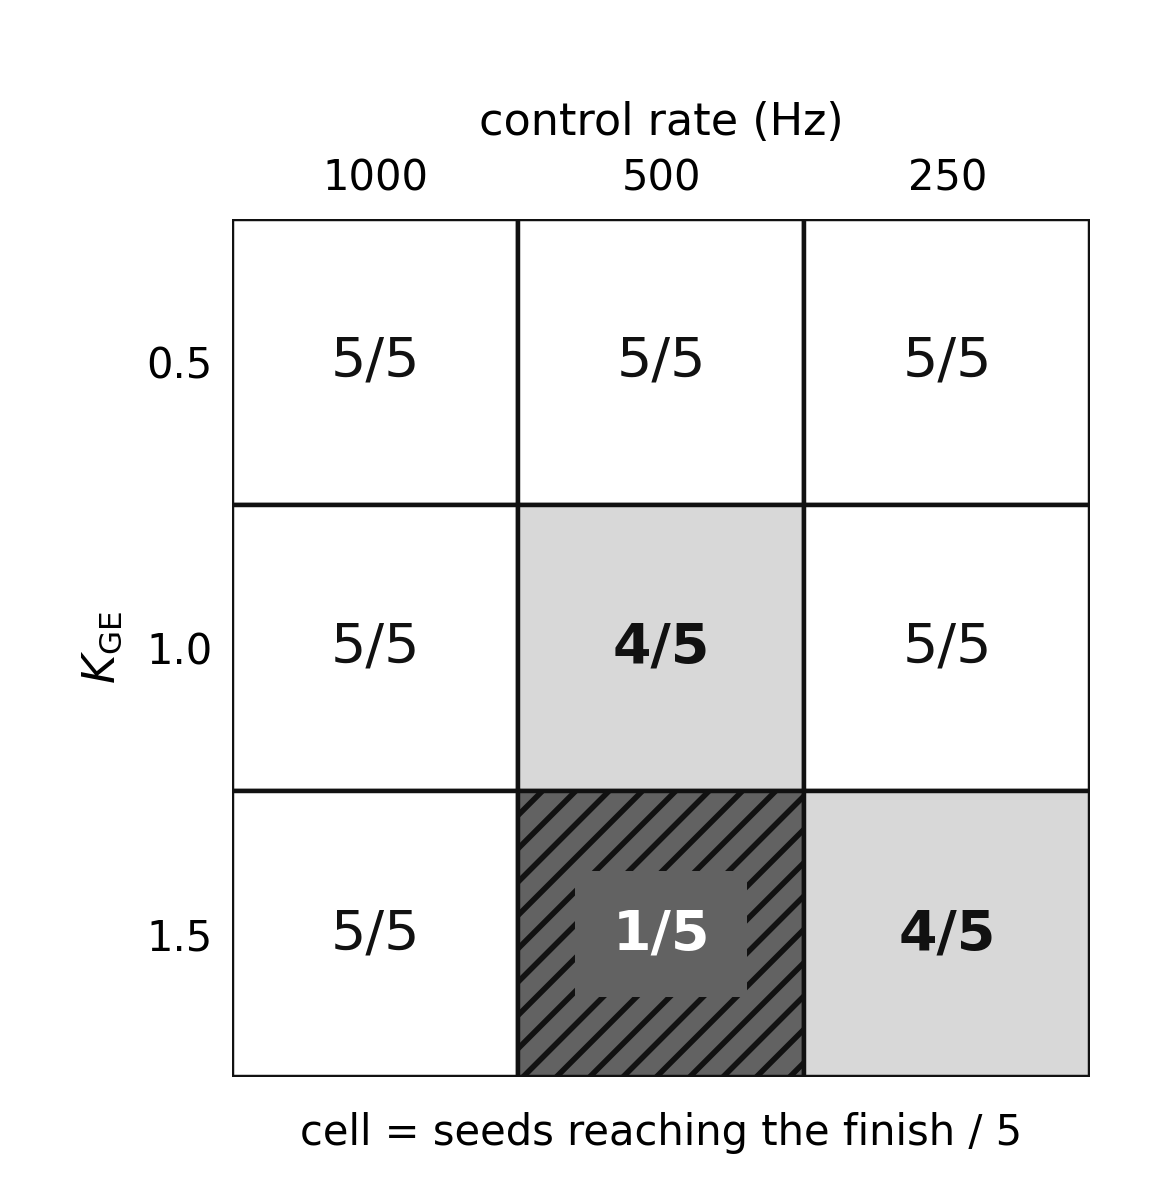
\includegraphics[width=0.85\linewidth]{figures/design_b_kge_grid_truewall.png}
\caption{Goal-reaching across ground-effect coefficient and control rate; each cell gives the number of noise realizations, out of five, that reached the goal.}
\label{fig:kge}
\end{figure}

\section{Discussion}
\label{sec:discussion}

This section interprets the results of Section~\ref{sec:results}, relates them to prior work, and states the implications, limitations, and directions for further study. The central question posed in Section~\ref{sec:introduction} was not only whether the wall-induced aerodynamic signal can be measured, but whether it contributes to the navigation task once a tactile cue is also present. The results answer the first part affirmatively and the second part conditionally: no contribution was detected beside an idealized tactile channel, and a clear one was confirmed once that channel's range was limited. The discussion is organized around that distinction.

\subsection{Interpretation of the Main Findings}
\label{sec:disc_interp}

Two findings stand together and must be read together. The characterization of Section~\ref{sec:results_sensor} shows that the wing-wash signal is, within the adopted model, a well-behaved proximity instrument: it is resolvable from roughly $8$ to $40$~mm and flyable from about $13$~mm, with a sub-millimetre noise-equivalent distance over most of that band, a stable observer gain, and a clean two-wall response. The ablation of Section~\ref{sec:results_ablation} and the paired analysis of Section~\ref{sec:results_stats} show that removing this signal from the integrated system changes performance by an amount that the experiments cannot distinguish from zero: the paired difference in strike-free completion was $+1.0$ percentage points with a confidence interval of $[-5.0, +6.5]$ and a $p$-value of $0.83$, and no difference was resolved on detection or clearance. The interval is not narrow: it is compatible with a benefit of up to about $6.5$ percentage points or a penalty of up to $5$, so the result is an absence of detected effect and not a demonstration of equivalence. Removing the tactile feelers, by contrast, reduced goal-reaching by more than half. The competence of the system is therefore attributable chiefly to the tactile channel, and the aerodynamic channel, though measurable, made no detectable contribution to the task in this regime.

This is a dissociation between what a signal \emph{is} and what it \emph{does}. The most direct explanation lies in the nature of the competing channel. The feelers modelled here are idealized: they return exact geometric range through free space, with only additive noise, and no dropout, deflection, or contact requirement. On the clean, rectilinear corridors of this study, such a channel supplies the centring and obstacle information the reactive controller needs with ample margin, leaving little for a second channel to add. The apparent redundancy is thus a property of the comparison as constructed, not a statement that the aerodynamic effect is without value in general. Consistent with this reading, the no-feelers configuration, in which lateral centring rests on the aerodynamic channel while the forward ray still governs speed and corner turns, reached the goal on $16$ of $40$ courses, against none in the open-loop case. Because the open-loop case also lacks the corner-turn trigger, this comparison does not isolate the aerodynamic channel, but it indicates that the signal can carry the centring task on some courses and is dominated when an idealized tactile cue is also available.

The confirmatory test of Section~\ref{sec:results_confirm} shows that this redundancy is conditional. With the feeler range limited to $0.05$~m, the aerodynamic channel raised strike-free completion by $16.5$ percentage points on $200$ new courses, with an interval of $[+8.5, +25.0]$ that excludes zero and lies above the $\pm 5$ point margin, and it raised goal-reaching, opening detection, and minimum clearance as well. The hypothesis came from one unplanned cell of an exploratory sweep, but the test that confirmed it was specified in advance, used courses that played no part in generating it, and returned an estimate close to the exploratory one. Its direction is the one the explanation above predicts, since it is when the tactile channel can no longer see the walls from a distance that a second, contactless channel would be expected to matter. A range of $0.05$~m is a little under twice the vehicle's span and is arguably closer to what a physical feeler could offer than the nominal $0.16$~m, so the regime in which the aerodynamic channel helps may be the more realistic of the two. The claim nonetheless remains narrow: it concerns one degradation axis at one level, with one noise seed per course, and at a limit of $0.03$~m both configurations failed on almost every course.

The gain sweep of Section~\ref{sec:results_gain} addresses the most direct objection to the null result with idealized feelers, namely that the channel is not redundant but under-used. Raising the centring gain up to eightfold produced no advantage and changed more individual outcomes in both directions, so the null result at the deployed gain is not explained by the size of that gain. The sweep is exploratory and leaves the roll saturation in place, and it does not test other uses of the signal, such as in the steering law, so it narrows this objection without closing it.

The width sweep of Section~\ref{sec:results_width} was meant to test a second objection, that the primary corridors keep the walls at the weak end of the signal's range and that the channel would matter where the walls are closer. It did not settle the matter. In the two narrowest bands every flight in both configurations struck a wall, so the pre-specified comparison was at the floor of its outcome and says nothing about the channel; what it does show is that the reactive layer, as tuned, cannot fly corridors narrower than about $58$~mm without striking, and that the aerodynamic channel does not rescue it there. In the three wider bands the strike-free difference showed no trend with width. The larger goal-reaching rate with the aerodynamic channel in the narrowest band is a single unadjusted secondary observation and is treated as a hypothesis, not a result.

\subsection{Relation to Prior Work}
\label{sec:disc_prior}

These findings connect closely to the two most relevant prior studies. Nakata et al.\ demonstrated that mosquitoes, and a bioinspired quadcopter, can detect surfaces from modifications of their self-induced airflow \cite{nakata2020aerodynamic}, establishing that aerodynamic surface sensing is physically real and useful on some platforms. The present study does not contradict this; it characterizes an analogous signal for a flapping-wing vehicle and confirms that it is measurable. What it adds is the separate question of marginal utility: whether, on a vehicle that also carries a tactile cue, the aerodynamic signal improves the task. The outcome here is conditional: no improvement was detected beside an idealized tactile channel, and a clear one was confirmed when the feeler range was limited to $0.05$~m. The caution this implies is also consistent with the hardware experience of Tu et al., who found no obvious wall effect in the current feedback of their flapping-wing platform and used wing contact instead \cite{tu2019acting}. Taken together, the prior work and the present study suggest that the existence of a near-wall aerodynamic effect does not by itself guarantee a useful navigational signal, and that whether it earns a place depends on the platform, the environment, and the alternative sensing available. The flapping-wing aerodynamics literature also reports a richer near-wall behaviour than the model contains, with force enhancement, reduction, and recovery as clearance decreases \cite{lu2016ground}. The saturating static response observed here does not correspond to those regimes; it follows from the cap in the adopted law, so the physical plausibility of the modelled signal rests on the distance dependence of the wall interaction in general and not on any agreement in its close-range form.

\subsection{Implications}
\label{sec:disc_implications}

The practical implication is a cautionary one for sensor design at this scale. A sensing modality can be accurately measurable, finely resolved, and physically well motivated, and still contribute nothing to a task if a simpler channel already suffices; evaluating a system only in its complete configuration will not reveal this, and can lead to a measurable-but-redundant signal being credited with a role it does not play. The ablation methodology used here, removing each channel on identical inputs and subjecting the comparison to a pre-specified paired test, is a general safeguard against that error, and its value was demonstrated concretely when it revealed that a simulation coupling had initially confounded the comparison. The converse error is equally possible: the same ablation, repeated with the competing channel degraded, showed the signal to be useful, so a verdict of redundancy is a statement about a pair of channels under stated conditions and not about one of them. The methodological implication, then, is that claims of sensory utility in such systems are best supported by ablation and by analysis that distinguishes measurability from contribution. On the positive side, the study establishes that control-only reactive navigation and opening inspection are achievable for a simulated insect-scale flapping-wing vehicle without vision, positioning, or learning, which is itself a useful baseline for confined-space operation.

\subsection{Limitations}
\label{sec:disc_limitations}

Several limitations bound these conclusions. First, the study is conducted entirely in simulation; no result has been shown to transfer to hardware, and the experience of prior investigators who found no obvious wall effect on a physical platform \cite{tu2019acting} underscores that this transfer is an open question. Second, the near-wall law of Eq.~\eqref{eq:kappa} is imposed rather than derived, and the sensitivity analysis of Section~\ref{sec:results_sensitivity} varies only the coefficient within that fixed functional form, so structural uncertainty in the form itself is untested. In particular, the law only ever enhances lift and omits the force-reduction regime reported for flapping wings at small clearance \cite{lu2016ground}; the saturation knee of the modelled response is produced by the cap $\kappa_{\max}$, and if a reduction regime extended into the flyable band, the modelled signal would be wrong there in magnitude and possibly in sign. Third, the sensor-noise model is an assumption, and the sub-millimetre resolution figure is a noise-equivalent distance under that assumption rather than a demonstrated sensor resolution. Fourth, and most consequentially for the central finding, the feeler model is idealized, and the null result is conditional on that idealization. A realistically imperfect tactile channel was approximated only through range limitation: the confirmed advantage was established at a single range limit of $0.05$~m, the $0.03$~m cell is incomplete, and the dropout and elevated-noise degradations were not evaluated. Fifth, the statistical basis is modest: a single noise realization for the noise floor, five for each cell of the detection-floor and sensitivity experiments, and, for the main comparison, five matched seeds across forty courses, sufficient to bound any benefit of the aerodynamic channel with idealized feelers at roughly $6.5$ percentage points of strike-free completion, but not to certify formal equivalence within the pre-specified margin. The confirmatory test used one noise seed on each of its $200$ courses, and the gain sweep is exploratory. The pre-specified comparison of the width sweep was uninformative, because strike-free completion was at its floor in the two narrowest bands; the choice of those bands for the primary comparison did not anticipate this, and the dependence of the aerodynamic contribution on corridor width therefore remains untested below about $58$~mm. The millimetre-level localization and sizing figures likewise come from a single straight corridor with one isolated opening; on the randomized courses the mean localization error was $7.9$~mm. Finally, the detection task concerns a geometric opening, not a specific hazard, and the correlation between an opening and a hazard is assumed from the application setting rather than measured. These limitations do not undermine the central, conditional dissociation, but they bound the range over which the reported numbers should be read as claims about a physical system.

\subsection{Future Research}
\label{sec:disc_future}

The limitations point directly to the work that would most advance this line. The confirmatory test establishes one point, at a feeler range of $0.05$~m, and the first and most promising experiment is to map the transition around it: range limits between $0.03$ and $0.08$~m with several noise seeds per course, together with the dropout, deflection, elevated-noise, and contact-limit degradations that were not evaluated, and on irregular rather than rectilinear walls. The question of corridor width should be put again with an outcome that is not at its floor in narrow corridors, such as strike count or time in contact, with the strike locations recorded, and after the navigation layer has been made able to fly them. The falsifiable hypothesis is that the aerodynamic channel's contribution rises steadily as the tactile channel is degraded toward physical realism, and that a regime exists in which it becomes necessary rather than merely helpful. The second is to test structural uncertainty in the near-wall law by comparing alternative functional forms, which would establish whether the sensing behaviour is a property of the wall interaction broadly or of the single form assumed. The third, and the one that would most raise the standing of the work, is a physical measurement: a tethered flapping-wing mechanism beside a movable wall, with the wall-induced roll disturbance measured against real sensor noise across distance and compared with the model. This would answer the question the simulation cannot, namely whether the signal exists at a usable magnitude on hardware, and would determine whether the modelled effect rests on a real physical signal or only on an assumed one. Together these three experiments would convert the present conditional result into a decisive statement about when a flapping wing's own aerodynamics are worth using to see.

\section{Conclusion}
\label{sec:conclusion}

This study investigated whether a flapping wing's near-wall aerodynamics can serve as a useful proximity sense for a confined-space micro air vehicle, using a physics-based simulation of a $77.4$~mg flapping-wing flyer controlled by a classical linear-quadratic-Gaussian regulator with a disturbance observer, and no learned policy, map, or external positioning. The wall-induced roll disturbance, recovered at no additional sensing cost from the controller's own observer, was shown to be a well-behaved proximity instrument within the adopted model, resolvable from roughly $8$ to $40$~mm and flyable from about $13$~mm, with a sub-millimetre noise-equivalent distance over most of that band, a stable observer gain, and a clean two-wall response. Built on this signal together with feelers, a purely reactive controller navigated confined corridors and detected isolated wall openings from about $12$~mm, localizing those up to $35$~mm long to within about a millimetre in a straight corridor. Across forty randomly generated multi-turn courses it reached the goal on $35$, without a wingtip strike on $30$, and detected $43$ of the $68$ openings with a mean localization error of $7.9$~mm.

The study's principal finding, however, was not the capability but the attribution of it. A controlled ablation, subjected to a pre-specified paired analysis on a corrected simulation harness, found that with idealized feelers removing the aerodynamic channel produced no detectable change in navigation or inspection performance, while removing feeler-based steering and wall avoidance more than halved goal-reaching. The confidence interval on that comparison, $[-5.0, +6.5]$ percentage points, does not establish formal equivalence, so a modest benefit cannot be excluded, and raising the centring gain up to eightfold did not produce one. A sweep of corridor width did not resolve whether closer walls change this, since in corridors narrower than about $58$~mm every flight in both configurations struck a wall. When the feeler range was limited to $0.05$~m, however, a confirmatory test on $200$ new courses found strike-free completion $16.5$ percentage points higher with the aerodynamic channel, with an interval of $[+8.5, +25.0]$, and goal-reaching, opening detection, and clearance improved with it. The wall-induced signal is therefore finely measurable throughout, makes no detectable contribution beside an idealized tactile channel, and makes a substantial one beside a range-limited channel, the most likely reason being that an idealized feeler already supplies what the reactive controller needs. This conditional dissociation between a signal that can be measured and a signal that contributes was detectable only because the comparison was made by ablation rather than by evaluating the complete system alone, and because the ablation was repeated with the competing channel degraded; it stands as a cautionary result, in both directions, for sensor design at this scale.

These findings remain bounded. They come from simulation, on rectilinear corridors, and the advantage is established at a single range limit with one noise seed per course. How the aerodynamic contribution varies across realistic tactile degradation, whether the modelled near-wall law holds in a different functional form, and whether the signal exists at a usable magnitude on hardware are the three questions that would decide the matter, and they define the natural continuation of this work.

\section*{Data availability}

The complete simulation framework, controller, experiment scripts, and generated datasets are available at \url{https://github.com/Ashfak-Kausik/flapping-flyer}, with each reported result reproducible from a frozen repository state.

%%%%%%%%%%%%%%%%%%%%%%%%%%%%%%%%%%%%%%%%%%%%%%%%%%%%%%%%%%%%
% BIBLIOGRAPHY
%%%%%%%%%%%%%%%%%%%%%%%%%%%%%%%%%%%%%%%%%%%%%%%%%%%%%%%%%%%%

\bibliographystyle{elsarticle-num}
\bibliography{references}

%%%%%%%%%%%%%%%%%%%%%%%%%%%%%%%%%%%%%%%%%%%%%%%%%%%%%%%%%%%%
\end{document}
